\documentclass{book}
\usepackage[a4paper,top=2.5cm,bottom=2.5cm,left=2.5cm,right=2.5cm]{geometry}
\usepackage{makeidx}
\usepackage{natbib}
\usepackage{graphicx}
\usepackage{multicol}
\usepackage{float}
\usepackage{listings}
\usepackage{color}
\usepackage{ifthen}
\usepackage[table]{xcolor}
\usepackage{textcomp}
\usepackage{alltt}
\usepackage{ifpdf}
\ifpdf
\usepackage[pdftex,
            pagebackref=true,
            colorlinks=true,
            linkcolor=blue,
            unicode
           ]{hyperref}
\else
\usepackage[ps2pdf,
            pagebackref=true,
            colorlinks=true,
            linkcolor=blue,
            unicode
           ]{hyperref}
\usepackage{pspicture}
\fi
\usepackage[utf8]{inputenc}
\usepackage{mathptmx}
\usepackage[scaled=.90]{helvet}
\usepackage{courier}
\usepackage{sectsty}
\usepackage{amssymb}
\usepackage[titles]{tocloft}
\usepackage{doxygen}
\lstset{language=C++,inputencoding=utf8,basicstyle=\footnotesize,breaklines=true,breakatwhitespace=true,tabsize=8,numbers=left }
\makeindex
\setcounter{tocdepth}{3}
\renewcommand{\footrulewidth}{0.4pt}
\renewcommand{\familydefault}{\sfdefault}
\hfuzz=15pt
\setlength{\emergencystretch}{15pt}
\hbadness=750
\tolerance=750
\begin{document}
\hypersetup{pageanchor=false,citecolor=blue}
\begin{titlepage}
\vspace*{7cm}
\begin{center}
{\Large D\-D2.5\-D \\[1ex]\large 0 }\\
\vspace*{1cm}
{\large Generated by Doxygen 1.8.2}\\
\vspace*{0.5cm}
{\small Thu May 2 2013 10:57:47}\\
\end{center}
\end{titlepage}
\clearemptydoublepage
\pagenumbering{roman}
\tableofcontents
\clearemptydoublepage
\pagenumbering{arabic}
\hypersetup{pageanchor=true,citecolor=blue}
\chapter{Hierarchical Index}
\section{\-Class \-Hierarchy}
\-This inheritance list is sorted roughly, but not completely, alphabetically\-:\begin{DoxyCompactList}
\item \contentsline{section}{\-Defect}{\pageref{d5/d4f/classDefect}}{}
\item \contentsline{section}{\-Matrix33}{\pageref{de/d82/classMatrix33}}{}
\begin{DoxyCompactList}
\item \contentsline{section}{\-Rotation\-Matrix}{\pageref{d2/d4a/classRotationMatrix}}{}
\item \contentsline{section}{\-Strain}{\pageref{d1/d3c/classStrain}}{}
\item \contentsline{section}{\-Stress}{\pageref{d1/d1c/classStress}}{}
\end{DoxyCompactList}
\item \contentsline{section}{\-Vector3d}{\pageref{df/dd0/classVector3d}}{}
\end{DoxyCompactList}

\chapter{Data Structure Index}
\section{\-Data \-Structures}
\-Here are the data structures with brief descriptions\-:\begin{DoxyCompactList}
\item\contentsline{section}{\hyperlink{classDefect}{\-Defect} }{\pageref{d5/d4f/classDefect}}{}
\item\contentsline{section}{\hyperlink{classMatrix33}{\-Matrix33} }{\pageref{de/d82/classMatrix33}}{}
\item\contentsline{section}{\hyperlink{classVector3d}{\-Vector3d} }{\pageref{df/dd0/classVector3d}}{}
\end{DoxyCompactList}

\chapter{File Index}
\section{\-File \-List}
\-Here is a list of all files with brief descriptions\-:\begin{DoxyCompactList}
\item\contentsline{section}{\hyperlink{constants_8h}{constants.\-h} \\*\-Definition of constants used in the program }{\pageref{d2/d6f/constants_8h}}{}
\item\contentsline{section}{\hyperlink{defect_8cpp}{defect.\-cpp} \\*\-Definition of member functions of the \hyperlink{classDefect}{\-Defect} class }{\pageref{dd/def/defect_8cpp}}{}
\item\contentsline{section}{\hyperlink{defect_8h}{defect.\-h} \\*\-Definition of the \hyperlink{classDefect}{\-Defect} class }{\pageref{df/d55/defect_8h}}{}
\item\contentsline{section}{\hyperlink{dislocation_8cpp}{dislocation.\-cpp} \\*\-Definition of constructors and member functions of the \hyperlink{classDislocation}{\-Dislocation} class }{\pageref{d3/d7f/dislocation_8cpp}}{}
\item\contentsline{section}{\hyperlink{dislocation_8h}{dislocation.\-h} \\*\-Definition of the \hyperlink{classDislocation}{\-Dislocation} class }{\pageref{de/df3/dislocation_8h}}{}
\item\contentsline{section}{\hyperlink{dislocationDefaults_8h}{dislocation\-Defaults.\-h} \\*\-Definition of certain default values for members of the \hyperlink{classDislocation}{\-Dislocation} class }{\pageref{d4/da6/dislocationDefaults_8h}}{}
\item\contentsline{section}{\hyperlink{dislocationSource_8cpp}{dislocation\-Source.\-cpp} \\*\-Definition of the member functions of the \hyperlink{classDislocationSource}{\-Dislocation\-Source} class }{\pageref{d8/d5c/dislocationSource_8cpp}}{}
\item\contentsline{section}{\hyperlink{dislocationSource_8h}{dislocation\-Source.\-h} \\*\-Definition of the \hyperlink{classDislocationSource}{\-Dislocation\-Source} class }{\pageref{da/d0c/dislocationSource_8h}}{}
\item\contentsline{section}{\hyperlink{dislocationSourceDefaults_8h}{dislocation\-Source\-Defaults.\-h} \\*\-Definition of certain default values for members of the \hyperlink{classDislocationSource}{\-Dislocation\-Source} class }{\pageref{d4/d0f/dislocationSourceDefaults_8h}}{}
\item\contentsline{section}{\hyperlink{matrix33_8cpp}{matrix33.\-cpp} \\*\-Definition of the member functions and operators of the \hyperlink{classMatrix33}{\-Matrix33} class }{\pageref{d8/d8e/matrix33_8cpp}}{}
\item\contentsline{section}{\hyperlink{matrix33_8h}{matrix33.\-h} \\*\-Definition of the \hyperlink{classMatrix33}{\-Matrix33} class }{\pageref{db/d46/matrix33_8h}}{}
\item\contentsline{section}{\hyperlink{parameter_8cpp}{parameter.\-cpp} \\*\-Definition of member functions of the \hyperlink{classParameter}{\-Parameter} class which will hold all simulation parameters }{\pageref{d4/d98/parameter_8cpp}}{}
\item\contentsline{section}{\hyperlink{parameter_8h}{parameter.\-h} \\*\-Declaration of the \hyperlink{classParameter}{\-Parameter} class which will hold all simulation parameters }{\pageref{d2/d2a/parameter_8h}}{}
\item\contentsline{section}{\hyperlink{rotationMatrix_8cpp}{rotation\-Matrix.\-cpp} \\*\-Definition of the \hyperlink{classRotationMatrix}{\-Rotation\-Matrix} class member functions }{\pageref{d9/d5c/rotationMatrix_8cpp}}{}
\item\contentsline{section}{\hyperlink{rotationMatrix_8h}{rotation\-Matrix.\-h} \\*\-Definition of the \hyperlink{classRotationMatrix}{\-Rotation\-Matrix} class }{\pageref{da/d76/rotationMatrix_8h}}{}
\item\contentsline{section}{\hyperlink{simulateSingleSlipPlane_8cpp}{simulate\-Single\-Slip\-Plane.\-cpp} \\*\-Defintion various functions to simulate dislocation motion on a single slip plane }{\pageref{d5/d1f/simulateSingleSlipPlane_8cpp}}{}
\item\contentsline{section}{\hyperlink{simulateSingleSlipPlane_8h}{simulate\-Single\-Slip\-Plane.\-h} \\*\-Declaration various functions to simulate dislocation motion on a single slip plane }{\pageref{d2/d56/simulateSingleSlipPlane_8h}}{}
\item\contentsline{section}{\hyperlink{slipPlane_8cpp}{slip\-Plane.\-cpp} \\*\-Definition of the member functions of the \hyperlink{classSlipPlane}{\-Slip\-Plane} class }{\pageref{db/dab/slipPlane_8cpp}}{}
\item\contentsline{section}{\hyperlink{slipPlane_8h}{slip\-Plane.\-h} \\*\-Definition of the \hyperlink{classSlipPlane}{\-Slip\-Plane} class }{\pageref{d5/d03/slipPlane_8h}}{}
\item\contentsline{section}{\hyperlink{slipPlaneDefaults_8h}{slip\-Plane\-Defaults.\-h} \\*\-Definition of certain default values for members of the \hyperlink{classSlipPlane}{\-Slip\-Plane} class }{\pageref{d1/d4f/slipPlaneDefaults_8h}}{}
\item\contentsline{section}{\hyperlink{standardSlipSystem_8cpp}{standard\-Slip\-System.\-cpp} \\*\-Definition of the member functions of the \hyperlink{classStandardSlipSystem}{\-Standard\-Slip\-System} class }{\pageref{d8/d92/standardSlipSystem_8cpp}}{}
\item\contentsline{section}{\hyperlink{standardSlipSystem_8h}{standard\-Slip\-System.\-h} \\*\-Definition of the \hyperlink{classStandardSlipSystem}{\-Standard\-Slip\-System} class }{\pageref{d0/ddd/standardSlipSystem_8h}}{}
\item\contentsline{section}{\hyperlink{statistics_8cpp}{statistics.\-cpp} \\*\-Definition of member functions of the \hyperlink{classStatistics}{\-Statistics} class which will hold the flag and frequency for various stastics }{\pageref{d1/d45/statistics_8cpp}}{}
\item\contentsline{section}{\hyperlink{statistics_8h}{statistics.\-h} \\*\-Declaration of the \hyperlink{classStatistics}{\-Statistics} class which will hold the flag and frequency for various stastics }{\pageref{d7/dc5/statistics_8h}}{}
\item\contentsline{section}{\hyperlink{strain_8cpp}{strain.\-cpp} \\*\-Definition of the member functions if the \hyperlink{classStrain}{\-Strain} class }{\pageref{d7/db1/strain_8cpp}}{}
\item\contentsline{section}{\hyperlink{strain_8h}{strain.\-h} \\*\-Definition of the \hyperlink{classStrain}{\-Strain} class }{\pageref{df/dc2/strain_8h}}{}
\item\contentsline{section}{\hyperlink{stress_8cpp}{stress.\-cpp} \\*\-Definition of the member functions if the \hyperlink{classStress}{\-Stress} class }{\pageref{d4/d58/stress_8cpp}}{}
\item\contentsline{section}{\hyperlink{stress_8h}{stress.\-h} \\*\-Definition of the \hyperlink{classStress}{\-Stress} class }{\pageref{d2/d50/stress_8h}}{}
\item\contentsline{section}{\hyperlink{tools_8cpp}{tools.\-cpp} \\*\-Definition various tools }{\pageref{d3/d62/tools_8cpp}}{}
\item\contentsline{section}{\hyperlink{tools_8h}{tools.\-h} \\*\-Declaration various tools }{\pageref{d5/da5/tools_8h}}{}
\item\contentsline{section}{\hyperlink{vector3d_8cpp}{vector3d.\-cpp} \\*\-Definition of member functions and operators of the \hyperlink{classVector3d}{\-Vector3d} class }{\pageref{d7/d35/vector3d_8cpp}}{}
\item\contentsline{section}{\hyperlink{vector3d_8h}{vector3d.\-h} \\*\-Definition of the \hyperlink{classVector3d}{\-Vector3d} class }{\pageref{d9/df8/vector3d_8h}}{}
\end{DoxyCompactList}

\chapter{Data Structure Documentation}
\hypertarget{classDefect}{\section{\-Defect \-Class \-Reference}
\label{d5/d4f/classDefect}\index{\-Defect@{\-Defect}}
}


\-Class \hyperlink{classDefect}{\-Defect} representing a generic defect in a material.  




{\ttfamily \#include $<$defect.\-h$>$}



\-Inheritance diagram for \-Defect\-:\nopagebreak
\begin{figure}[H]
\begin{center}
\leavevmode
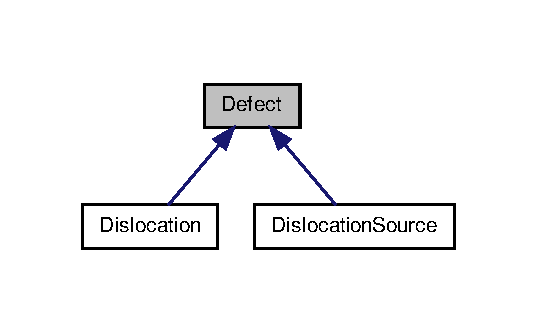
\includegraphics[width=144pt]{de/d48/classDefect__inherit__graph}
\end{center}
\end{figure}


\-Collaboration diagram for \-Defect\-:\nopagebreak
\begin{figure}[H]
\begin{center}
\leavevmode
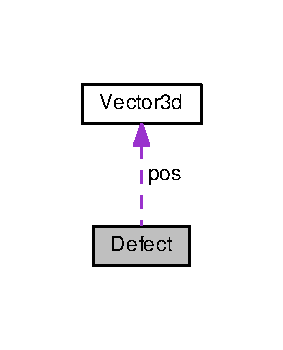
\includegraphics[width=136pt]{d7/d09/classDefect__coll__graph}
\end{center}
\end{figure}
\subsection*{\-Public \-Member \-Functions}
\begin{DoxyCompactItemize}
\item 
\hyperlink{classDefect_afc84dd2d7250a01746ee67b002dbbad9}{\-Defect} ()
\begin{DoxyCompactList}\small\item\em \-Default constructor. \end{DoxyCompactList}\item 
\hyperlink{classDefect_aaddcb1db4b47037adf2e495665f41bab}{\-Defect} (double x, double y, double z)
\begin{DoxyCompactList}\small\item\em \-Constructor specifying the position. \end{DoxyCompactList}\item 
\hyperlink{classDefect_a5bd123214102a5115c46b0a15653d29b}{\-Defect} (double $\ast$p)
\begin{DoxyCompactList}\small\item\em \-Constructor specifying the position. \end{DoxyCompactList}\item 
void \hyperlink{classDefect_a2d233d13a8a93f6fba463a1fbc1c6c9f}{set\-Position} (double $\ast$a)
\begin{DoxyCompactList}\small\item\em \-Sets the position of the defect. \end{DoxyCompactList}\item 
void \hyperlink{classDefect_ad1a6acd8399d2ecabb7ce2b77623bbec}{set\-Position} (double x, double y, double z)
\begin{DoxyCompactList}\small\item\em \-Sets the position of the defect. \end{DoxyCompactList}\item 
void \hyperlink{classDefect_a5a65f73da6a572d9e7109b31239e441d}{set\-X} (double x)
\begin{DoxyCompactList}\small\item\em \-Sets the \-X-\/coordinate of the defect. \end{DoxyCompactList}\item 
void \hyperlink{classDefect_a268606391a4eaee3de029d2005648b6f}{set\-Y} (double y)
\begin{DoxyCompactList}\small\item\em \-Sets the \-Y-\/coordinate of the defect. \end{DoxyCompactList}\item 
void \hyperlink{classDefect_abb0b16c44a1b04d782f5c5f598b49d5b}{set\-Z} (double z)
\begin{DoxyCompactList}\small\item\em \-Sets the \-Z-\/coordinate of the defect. \end{DoxyCompactList}\item 
double $\ast$ \hyperlink{classDefect_a6842fba3ad14032766ccf0437afcbced}{get\-Position} ()
\begin{DoxyCompactList}\small\item\em \-Returns in an array the position. \end{DoxyCompactList}\item 
void \hyperlink{classDefect_aace5c752b85c368631746abc3d5bd714}{get\-Position} (double $\ast$a)
\begin{DoxyCompactList}\small\item\em \-Returns the array position in a pre-\/allocated array. \end{DoxyCompactList}\item 
double \hyperlink{classDefect_a01b96c453c13db82b5835682e1849dc0}{get\-X} ()
\begin{DoxyCompactList}\small\item\em \-Returns the \-X-\/coordinate of the defect. \end{DoxyCompactList}\item 
double \hyperlink{classDefect_a9ea8df3b4c621762a327813056e63911}{get\-Y} ()
\begin{DoxyCompactList}\small\item\em \-Returns the \-Y-\/coordinate of the defect. \end{DoxyCompactList}\item 
double \hyperlink{classDefect_a6f59edeca7ca8bfa01c54fd6b1a62374}{get\-Z} ()
\begin{DoxyCompactList}\small\item\em \-Returns the \-Z-\/coordinate of the defect. \end{DoxyCompactList}\item 
virtual \hyperlink{classStress}{\-Stress} \hyperlink{classDefect_af25282562571e6fe3340e82d02c7ae93}{stress\-Field} (\hyperlink{classVector3d}{\-Vector3d} p)
\begin{DoxyCompactList}\small\item\em \-Virtual function for calculating the stress field. \end{DoxyCompactList}\end{DoxyCompactItemize}
\subsection*{\-Protected \-Attributes}
\begin{DoxyCompactItemize}
\item 
\hyperlink{classVector3d}{\-Vector3d} \hyperlink{classDefect_aed2731c1beefc22e3db6ad5b18194cdd}{pos}
\begin{DoxyCompactList}\small\item\em \-Position vector of the defect in 2\-D space. \end{DoxyCompactList}\end{DoxyCompactItemize}


\subsection{\-Detailed \-Description}
\-Class \hyperlink{classDefect}{\-Defect} representing a generic defect in a material. 

\-Defines the \hyperlink{classDefect}{\-Defect} class representing an defect in the simulation. \-This is simply a generic description class with virtual functions. \-Later classes like dislocations, precipitates, boundaries etc will inherit from this class. 

\-Definition at line 23 of file defect.\-h.



\subsection{\-Constructor \& \-Destructor \-Documentation}
\hypertarget{classDefect_afc84dd2d7250a01746ee67b002dbbad9}{\index{\-Defect@{\-Defect}!\-Defect@{\-Defect}}
\index{\-Defect@{\-Defect}!Defect@{\-Defect}}
\subsubsection[{\-Defect}]{\setlength{\rightskip}{0pt plus 5cm}{\bf \-Defect\-::\-Defect} (
\begin{DoxyParamCaption}
{}
\end{DoxyParamCaption}
)}}\label{d5/d4f/classDefect_afc84dd2d7250a01746ee67b002dbbad9}


\-Default constructor. 

\-Creates the object with position (0.\-0, 0.\-0, 0.\-0). 

\-Definition at line 17 of file defect.\-cpp.


\begin{DoxyCode}
{
  for (int i=0; i<3; i++)
    {
      this->pos.setValue(i, 0.0);
    }
}
\end{DoxyCode}
\hypertarget{classDefect_aaddcb1db4b47037adf2e495665f41bab}{\index{\-Defect@{\-Defect}!\-Defect@{\-Defect}}
\index{\-Defect@{\-Defect}!Defect@{\-Defect}}
\subsubsection[{\-Defect}]{\setlength{\rightskip}{0pt plus 5cm}{\bf \-Defect\-::\-Defect} (
\begin{DoxyParamCaption}
\item[{double}]{x, }
\item[{double}]{y, }
\item[{double}]{z}
\end{DoxyParamCaption}
)}}\label{d5/d4f/classDefect_aaddcb1db4b47037adf2e495665f41bab}


\-Constructor specifying the position. 

\-The object is initialized with the position specified by the arguments (x, y, z). 
\begin{DoxyParams}{\-Parameters}
{\em x} & \-X-\/coordinate of the defect. \\
\hline
{\em y} & \-Y-\/coordinate of the defect \\
\hline
{\em z} & \-Z-\/coordinate of the defect. \\
\hline
\end{DoxyParams}


\-Definition at line 32 of file defect.\-cpp.


\begin{DoxyCode}
{
  this->pos.setValue (0, x);
  this->pos.setValue (1, y);
  this->pos.setValue (2, z);
}
\end{DoxyCode}
\hypertarget{classDefect_a5bd123214102a5115c46b0a15653d29b}{\index{\-Defect@{\-Defect}!\-Defect@{\-Defect}}
\index{\-Defect@{\-Defect}!Defect@{\-Defect}}
\subsubsection[{\-Defect}]{\setlength{\rightskip}{0pt plus 5cm}{\bf \-Defect\-::\-Defect} (
\begin{DoxyParamCaption}
\item[{double $\ast$}]{p}
\end{DoxyParamCaption}
)}}\label{d5/d4f/classDefect_a5bd123214102a5115c46b0a15653d29b}


\-Constructor specifying the position. 

\-The object is initialized with the position specified in the array pointed to by the argument. 
\begin{DoxyParams}{\-Parameters}
{\em p} & \-Pointer to the array containing the coordinates of the defect. \\
\hline
\end{DoxyParams}


\-Definition at line 44 of file defect.\-cpp.


\begin{DoxyCode}
{
  this->pos.setValue (p);
}
\end{DoxyCode}


\subsection{\-Member \-Function \-Documentation}
\hypertarget{classDefect_a6842fba3ad14032766ccf0437afcbced}{\index{\-Defect@{\-Defect}!get\-Position@{get\-Position}}
\index{get\-Position@{get\-Position}!Defect@{\-Defect}}
\subsubsection[{get\-Position}]{\setlength{\rightskip}{0pt plus 5cm}double $\ast$ {\bf \-Defect\-::get\-Position} (
\begin{DoxyParamCaption}
{}
\end{DoxyParamCaption}
)}}\label{d5/d4f/classDefect_a6842fba3ad14032766ccf0437afcbced}


\-Returns in an array the position. 

\-The position of the defect is saved in an array and a pointer to its first term is returned. \begin{DoxyReturn}{\-Returns}
\-Pointer to the first term of the array containing the position of the defect. 
\end{DoxyReturn}


\-Definition at line 109 of file defect.\-cpp.


\begin{DoxyCode}
{
  return (this->pos.getVector ());
}
\end{DoxyCode}
\hypertarget{classDefect_aace5c752b85c368631746abc3d5bd714}{\index{\-Defect@{\-Defect}!get\-Position@{get\-Position}}
\index{get\-Position@{get\-Position}!Defect@{\-Defect}}
\subsubsection[{get\-Position}]{\setlength{\rightskip}{0pt plus 5cm}void {\bf \-Defect\-::get\-Position} (
\begin{DoxyParamCaption}
\item[{double $\ast$}]{a}
\end{DoxyParamCaption}
)}}\label{d5/d4f/classDefect_aace5c752b85c368631746abc3d5bd714}


\-Returns the array position in a pre-\/allocated array. 

\-Returns in the array provided in the argument the position of the defect. \-The array must be pre-\/allocated. 
\begin{DoxyParams}{\-Parameters}
{\em a} & \-Pointer to the location where the defect coordinates are to be populated. \\
\hline
\end{DoxyParams}


\-Definition at line 119 of file defect.\-cpp.


\begin{DoxyCode}
{
  a = this->pos.getVector ();
}
\end{DoxyCode}
\hypertarget{classDefect_a01b96c453c13db82b5835682e1849dc0}{\index{\-Defect@{\-Defect}!get\-X@{get\-X}}
\index{get\-X@{get\-X}!Defect@{\-Defect}}
\subsubsection[{get\-X}]{\setlength{\rightskip}{0pt plus 5cm}double {\bf \-Defect\-::get\-X} (
\begin{DoxyParamCaption}
{}
\end{DoxyParamCaption}
)}}\label{d5/d4f/classDefect_a01b96c453c13db82b5835682e1849dc0}


\-Returns the \-X-\/coordinate of the defect. 

\begin{DoxyReturn}{\-Returns}
\-X-\/coordinate of the defect. 
\end{DoxyReturn}


\-Definition at line 128 of file defect.\-cpp.


\begin{DoxyCode}
{
  return (this->getValue (0));
}
\end{DoxyCode}
\hypertarget{classDefect_a9ea8df3b4c621762a327813056e63911}{\index{\-Defect@{\-Defect}!get\-Y@{get\-Y}}
\index{get\-Y@{get\-Y}!Defect@{\-Defect}}
\subsubsection[{get\-Y}]{\setlength{\rightskip}{0pt plus 5cm}double {\bf \-Defect\-::get\-Y} (
\begin{DoxyParamCaption}
{}
\end{DoxyParamCaption}
)}}\label{d5/d4f/classDefect_a9ea8df3b4c621762a327813056e63911}


\-Returns the \-Y-\/coordinate of the defect. 

\begin{DoxyReturn}{\-Returns}
\-Y-\/coordinate of the defect. 
\end{DoxyReturn}


\-Definition at line 137 of file defect.\-cpp.


\begin{DoxyCode}
{
  return (this->pos.getValue (1));
}
\end{DoxyCode}
\hypertarget{classDefect_a6f59edeca7ca8bfa01c54fd6b1a62374}{\index{\-Defect@{\-Defect}!get\-Z@{get\-Z}}
\index{get\-Z@{get\-Z}!Defect@{\-Defect}}
\subsubsection[{get\-Z}]{\setlength{\rightskip}{0pt plus 5cm}double {\bf \-Defect\-::get\-Z} (
\begin{DoxyParamCaption}
{}
\end{DoxyParamCaption}
)}}\label{d5/d4f/classDefect_a6f59edeca7ca8bfa01c54fd6b1a62374}


\-Returns the \-Z-\/coordinate of the defect. 

\begin{DoxyReturn}{\-Returns}
\-Z-\/coordinate of the defect. 
\end{DoxyReturn}


\-Definition at line 146 of file defect.\-cpp.


\begin{DoxyCode}
{
  return (this->pos.getValue (2));
}
\end{DoxyCode}
\hypertarget{classDefect_a2d233d13a8a93f6fba463a1fbc1c6c9f}{\index{\-Defect@{\-Defect}!set\-Position@{set\-Position}}
\index{set\-Position@{set\-Position}!Defect@{\-Defect}}
\subsubsection[{set\-Position}]{\setlength{\rightskip}{0pt plus 5cm}void {\bf \-Defect\-::set\-Position} (
\begin{DoxyParamCaption}
\item[{double $\ast$}]{a}
\end{DoxyParamCaption}
)}}\label{d5/d4f/classDefect_a2d233d13a8a93f6fba463a1fbc1c6c9f}


\-Sets the position of the defect. 

\-The position of the defect is set to the co-\/ordinates present in the array pointed to by the argument. \-Sets the position of the defect as the values in the array pointed to by the argument. 
\begin{DoxyParams}{\-Parameters}
{\em a} & \-Pointer to the array containing the coordinates of the defect. \\
\hline
\end{DoxyParams}


\-Definition at line 56 of file defect.\-cpp.


\begin{DoxyCode}
{
  this->pos.setValue (a);
}
\end{DoxyCode}
\hypertarget{classDefect_ad1a6acd8399d2ecabb7ce2b77623bbec}{\index{\-Defect@{\-Defect}!set\-Position@{set\-Position}}
\index{set\-Position@{set\-Position}!Defect@{\-Defect}}
\subsubsection[{set\-Position}]{\setlength{\rightskip}{0pt plus 5cm}void {\bf \-Defect\-::set\-Position} (
\begin{DoxyParamCaption}
\item[{double}]{x, }
\item[{double}]{y, }
\item[{double}]{z}
\end{DoxyParamCaption}
)}}\label{d5/d4f/classDefect_ad1a6acd8399d2ecabb7ce2b77623bbec}


\-Sets the position of the defect. 

\-The position of the defect is set to the co-\/ordinates specified by the arguments (x, y, z). \-Sets the position of the defect as the coordinates provided as arguments. 
\begin{DoxyParams}{\-Parameters}
{\em x} & \-X-\/coordinate of the defect. \\
\hline
{\em y} & \-Y-\/coordinate of the defect. \\
\hline
{\em z} & \-Z-\/coordinate of the defect. \\
\hline
\end{DoxyParams}


\-Definition at line 69 of file defect.\-cpp.


\begin{DoxyCode}
{
  this->pos.setValue (0, x);
  this->pos.setValue (1, y);
  this->pos.setValue (2, z);
}
\end{DoxyCode}
\hypertarget{classDefect_a5a65f73da6a572d9e7109b31239e441d}{\index{\-Defect@{\-Defect}!set\-X@{set\-X}}
\index{set\-X@{set\-X}!Defect@{\-Defect}}
\subsubsection[{set\-X}]{\setlength{\rightskip}{0pt plus 5cm}void {\bf \-Defect\-::set\-X} (
\begin{DoxyParamCaption}
\item[{double}]{x}
\end{DoxyParamCaption}
)}}\label{d5/d4f/classDefect_a5a65f73da6a572d9e7109b31239e441d}


\-Sets the \-X-\/coordinate of the defect. 


\begin{DoxyParams}{\-Parameters}
{\em x} & \-X-\/coordinate of the defect. \\
\hline
\end{DoxyParams}


\-Definition at line 80 of file defect.\-cpp.


\begin{DoxyCode}
{
  this->pos.setValue (0, x);
}
\end{DoxyCode}
\hypertarget{classDefect_a268606391a4eaee3de029d2005648b6f}{\index{\-Defect@{\-Defect}!set\-Y@{set\-Y}}
\index{set\-Y@{set\-Y}!Defect@{\-Defect}}
\subsubsection[{set\-Y}]{\setlength{\rightskip}{0pt plus 5cm}void {\bf \-Defect\-::set\-Y} (
\begin{DoxyParamCaption}
\item[{double}]{y}
\end{DoxyParamCaption}
)}}\label{d5/d4f/classDefect_a268606391a4eaee3de029d2005648b6f}


\-Sets the \-Y-\/coordinate of the defect. 


\begin{DoxyParams}{\-Parameters}
{\em y} & \-Y-\/coordinate of the defect. \\
\hline
\end{DoxyParams}


\-Definition at line 89 of file defect.\-cpp.


\begin{DoxyCode}
{
  this->pos.setValue (1, y);
}
\end{DoxyCode}
\hypertarget{classDefect_abb0b16c44a1b04d782f5c5f598b49d5b}{\index{\-Defect@{\-Defect}!set\-Z@{set\-Z}}
\index{set\-Z@{set\-Z}!Defect@{\-Defect}}
\subsubsection[{set\-Z}]{\setlength{\rightskip}{0pt plus 5cm}void {\bf \-Defect\-::set\-Z} (
\begin{DoxyParamCaption}
\item[{double}]{z}
\end{DoxyParamCaption}
)}}\label{d5/d4f/classDefect_abb0b16c44a1b04d782f5c5f598b49d5b}


\-Sets the \-Z-\/coordinate of the defect. 


\begin{DoxyParams}{\-Parameters}
{\em z} & \-Z-\/coordinate of the defect. \\
\hline
\end{DoxyParams}


\-Definition at line 98 of file defect.\-cpp.


\begin{DoxyCode}
{
  this->pos.setValue (2, z);
}
\end{DoxyCode}
\hypertarget{classDefect_af25282562571e6fe3340e82d02c7ae93}{\index{\-Defect@{\-Defect}!stress\-Field@{stress\-Field}}
\index{stress\-Field@{stress\-Field}!Defect@{\-Defect}}
\subsubsection[{stress\-Field}]{\setlength{\rightskip}{0pt plus 5cm}virtual {\bf \-Stress} {\bf \-Defect\-::stress\-Field} (
\begin{DoxyParamCaption}
\item[{{\bf \-Vector3d}}]{p}
\end{DoxyParamCaption}
)\hspace{0.3cm}{\ttfamily  \mbox{[}inline, virtual\mbox{]}}}}\label{d5/d4f/classDefect_af25282562571e6fe3340e82d02c7ae93}


\-Virtual function for calculating the stress field. 

\-Returns the value of the stress field of the given defect at the position given by the argument. \-This is a virtual function and always returns a zero matrix. \-Classes which inherit this function should have their own implementations of this function to override its behaviour. 
\begin{DoxyParams}{\-Parameters}
{\em p} & \-Position vector of the the point where the stress field is to be calculated. \\
\hline
\end{DoxyParams}
\begin{DoxyReturn}{\-Returns}
\hyperlink{classStress}{\-Stress} field value at the position p. 
\end{DoxyReturn}


\-Definition at line 122 of file defect.\-h.


\begin{DoxyCode}
  {
    // This virtual function returns a zero matrix.
    // Inheriting classes will have functions implementing this in their own
       way
    // They will override this behaviour.
    Stress s;
    return (s);
  }
\end{DoxyCode}


\subsection{\-Field \-Documentation}
\hypertarget{classDefect_aed2731c1beefc22e3db6ad5b18194cdd}{\index{\-Defect@{\-Defect}!pos@{pos}}
\index{pos@{pos}!Defect@{\-Defect}}
\subsubsection[{pos}]{\setlength{\rightskip}{0pt plus 5cm}{\bf \-Vector3d} {\bf \-Defect\-::pos}\hspace{0.3cm}{\ttfamily  \mbox{[}protected\mbox{]}}}}\label{d5/d4f/classDefect_aed2731c1beefc22e3db6ad5b18194cdd}


\-Position vector of the defect in 2\-D space. 



\-Definition at line 29 of file defect.\-h.



\-The documentation for this class was generated from the following files\-:\begin{DoxyCompactItemize}
\item 
\hyperlink{defect_8h}{defect.\-h}\item 
\hyperlink{defect_8cpp}{defect.\-cpp}\end{DoxyCompactItemize}

\hypertarget{classDislocation}{\section{\-Dislocation \-Class \-Reference}
\label{d3/dc6/classDislocation}\index{\-Dislocation@{\-Dislocation}}
}


\hyperlink{classDislocation}{\-Dislocation} class representing a dislocation in the simulation.  




{\ttfamily \#include $<$dislocation.\-h$>$}



\-Inheritance diagram for \-Dislocation\-:
\nopagebreak
\begin{figure}[H]
\begin{center}
\leavevmode
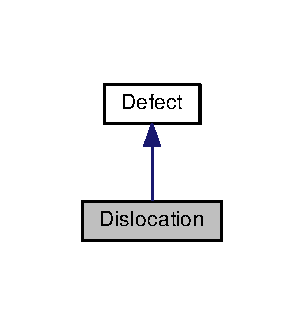
\includegraphics[width=144pt]{df/dfa/classDislocation__inherit__graph}
\end{center}
\end{figure}


\-Collaboration diagram for \-Dislocation\-:
\nopagebreak
\begin{figure}[H]
\begin{center}
\leavevmode
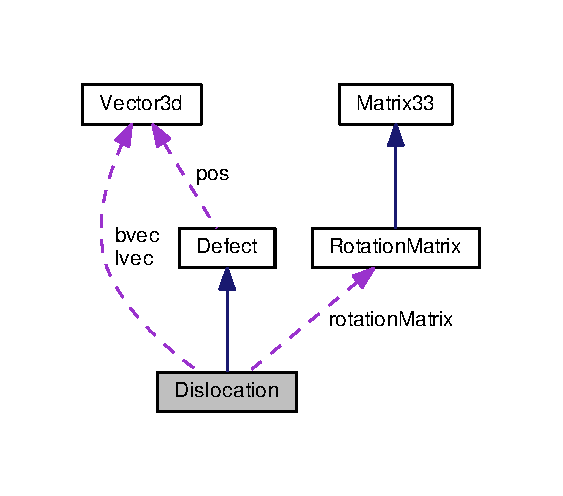
\includegraphics[width=350pt]{d7/d80/classDislocation__coll__graph}
\end{center}
\end{figure}
\subsection*{\-Public \-Member \-Functions}
\begin{DoxyCompactItemize}
\item 
\hyperlink{classDislocation_ac5eed47d88651f3f2ed7f090036f804e}{\-Dislocation} ()
\begin{DoxyCompactList}\small\item\em \-Default constructor. \end{DoxyCompactList}\item 
\hyperlink{classDislocation_a332cb83378000624b6eea474ca31a8c2}{\-Dislocation} (\hyperlink{classVector3d}{\-Vector3d} burgers, \hyperlink{classVector3d}{\-Vector3d} line, \hyperlink{classVector3d}{\-Vector3d} position, double bm, bool m)
\begin{DoxyCompactList}\small\item\em \-Constructor that explicitly specifies all parameters. \end{DoxyCompactList}\item 
void \hyperlink{classDislocation_ab827fcf321729c1238caaa3bceff323a}{set\-Burgers} (\hyperlink{classVector3d}{\-Vector3d} burgers)
\begin{DoxyCompactList}\small\item\em \-Sets the \-Burgers vector of the dislocation. \end{DoxyCompactList}\item 
void \hyperlink{classDislocation_a6e814df21c8dfbd1e2e8f492673a79b2}{set\-Line\-Vector} (\hyperlink{classVector3d}{\-Vector3d} line)
\begin{DoxyCompactList}\small\item\em \-Sets the line vector of the dislocation. \end{DoxyCompactList}\item 
void \hyperlink{classDislocation_a59d404cb0d3dbaaa3380e4fd4018c4d3}{set\-Mobile} ()
\begin{DoxyCompactList}\small\item\em \-Sets the dislocation as mobile. \end{DoxyCompactList}\item 
void \hyperlink{classDislocation_a769db83b0546e7785b5890a5979a8d82}{set\-Pinned} ()
\begin{DoxyCompactList}\small\item\em \-Sets the dislocation as pinned. \end{DoxyCompactList}\item 
void \hyperlink{classDislocation_acc1b0c77cc1150cc7d6d7bc098acb610}{set\-Total\-Stress} (\hyperlink{classStress}{\-Stress} s)
\begin{DoxyCompactList}\small\item\em \-Sets the total stress value in the class and the vector keeping track of stresses in each iteration. \end{DoxyCompactList}\item 
void \hyperlink{classDislocation_aebe391b1ed71cd98b506abbdd493fc31}{set\-Total\-Force} (\hyperlink{classVector3d}{\-Vector3d} f)
\begin{DoxyCompactList}\small\item\em \-Sets the total force in the class and the vector keeping track of forces in each iteration. \end{DoxyCompactList}\item 
void \hyperlink{classDislocation_aeb55f4d1364d2e33891e41868592c629}{set\-Velocity} (\hyperlink{classVector3d}{\-Vector3d} v)
\begin{DoxyCompactList}\small\item\em \-Sets the total velocity in the class and the vector keeping track of velocities in each iteration. \end{DoxyCompactList}\item 
\hyperlink{classVector3d}{\-Vector3d} \hyperlink{classDislocation_a9eb3cc78d08d26a29d5f318a33f6065e}{get\-Burgers} () const 
\begin{DoxyCompactList}\small\item\em \-Gets the \-Burgers vector of the dislocation. \end{DoxyCompactList}\item 
\hyperlink{classVector3d}{\-Vector3d} \hyperlink{classDislocation_a8ba2d0d68c7b335e5c75b7498b33803d}{get\-Line\-Vector} () const 
\begin{DoxyCompactList}\small\item\em \-Gets the line vector of the dislocation. \end{DoxyCompactList}\item 
bool \hyperlink{classDislocation_a741fe1113b1693a6b2f3ad364e9508fe}{is\-Mobile} () const 
\begin{DoxyCompactList}\small\item\em \-Returns whether the dislocation is mobile or pinned. \end{DoxyCompactList}\item 
\hyperlink{classStress}{\-Stress} \hyperlink{classDislocation_a2e07940bcbec8e998f31769f9cc0f5f2}{get\-Total\-Stress} () const 
\begin{DoxyCompactList}\small\item\em \-Gets the total stress in the current iteration. \end{DoxyCompactList}\item 
\hyperlink{classVector3d}{\-Vector3d} \hyperlink{classDislocation_a826a6aae1035b454cfc42db4bb863a4d}{get\-Total\-Force} () const 
\begin{DoxyCompactList}\small\item\em \-Gets the total force on the dislocation in the current iteration. \end{DoxyCompactList}\item 
\hyperlink{classVector3d}{\-Vector3d} \hyperlink{classDislocation_a74b8029dd76a9a43ac437aa144132a72}{get\-Velocity} () const 
\begin{DoxyCompactList}\small\item\em \-The velocity of the dislocation in the current iteration. \end{DoxyCompactList}\item 
\hyperlink{classStress}{\-Stress} \hyperlink{classDislocation_af57a21490312108d68540544596cc7a7}{get\-Total\-Stress\-At\-Iteration} (int i) const 
\begin{DoxyCompactList}\small\item\em \-Returns the total stress at the iteration i. \end{DoxyCompactList}\item 
\hyperlink{classVector3d}{\-Vector3d} \hyperlink{classDislocation_a2a693d6e986cf0d8bed2a55e6ce721bd}{get\-Total\-Force\-At\-Iteration} (int i) const 
\begin{DoxyCompactList}\small\item\em \-Returns the total force at the iteration i. \end{DoxyCompactList}\item 
\hyperlink{classVector3d}{\-Vector3d} \hyperlink{classDislocation_a6cf00cadeb4b42c4b3126d15137d1f04}{get\-Velocity\-At\-Iteration} (int i) const 
\begin{DoxyCompactList}\small\item\em \-Returns the total velocity at the iteration i. \end{DoxyCompactList}\item 
void \hyperlink{classDislocation_aa249f1f46486fd183757ed5049586e73}{calculate\-Rotation\-Matrix} ()
\begin{DoxyCompactList}\small\item\em \-Calculate the roation matrix. \end{DoxyCompactList}\item 
\hyperlink{classStress}{\-Stress} \hyperlink{classDislocation_af61cedf5305080ce0f55eb7177efe529}{stress\-Field} (\hyperlink{classVector3d}{\-Vector3d} p, double mu, double nu)
\begin{DoxyCompactList}\small\item\em \-Calculates the stress field due to this dislocation at the position given as argument. \end{DoxyCompactList}\item 
\hyperlink{classStress}{\-Stress} \hyperlink{classDislocation_a26f938bfb630c3ba1b13522d7a422b8c}{stress\-Field\-Local} (\hyperlink{classVector3d}{\-Vector3d} p, double mu, double nu) const 
\begin{DoxyCompactList}\small\item\em \-Calculates the stress field due to the dislocation in the local co-\/ordinate system. \end{DoxyCompactList}\item 
\hyperlink{classVector3d}{\-Vector3d} \hyperlink{classDislocation_a9ca3f6fb280edaa1fbf156d75b8f0527}{force\-Peach\-Koehler} (\hyperlink{classStress}{\-Stress} sigma, double tau\-\_\-crss) const 
\begin{DoxyCompactList}\small\item\em \-Calculate the \-Peach-\/\-Koehler force acting on the dislocation due the stress. \end{DoxyCompactList}\item 
double \hyperlink{classDislocation_a6b02065fa97acefac00400182dea8738}{ideal\-Time\-Increment} (double min\-Distance, \hyperlink{classDefect}{\-Defect} d, \hyperlink{classVector3d}{\-Vector3d} v1)
\begin{DoxyCompactList}\small\item\em \-Returns the ideal time increment for the dislocation. \end{DoxyCompactList}\item 
void \hyperlink{classDefect_a2d233d13a8a93f6fba463a1fbc1c6c9f}{set\-Position} (double $\ast$a)
\begin{DoxyCompactList}\small\item\em \-Sets the position of the defect. \end{DoxyCompactList}\item 
void \hyperlink{classDefect_ad1a6acd8399d2ecabb7ce2b77623bbec}{set\-Position} (double x, double y, double z)
\begin{DoxyCompactList}\small\item\em \-Sets the position of the defect. \end{DoxyCompactList}\item 
void \hyperlink{classDefect_a36ffa9b4b01d38ed8a95ca2c78973cc4}{set\-Position} (\hyperlink{classVector3d}{\-Vector3d} a)
\begin{DoxyCompactList}\small\item\em \-Sets the position of the defect. \end{DoxyCompactList}\item 
void \hyperlink{classDefect_a5a65f73da6a572d9e7109b31239e441d}{set\-X} (double x)
\begin{DoxyCompactList}\small\item\em \-Sets the \-X-\/coordinate of the defect. \end{DoxyCompactList}\item 
void \hyperlink{classDefect_a268606391a4eaee3de029d2005648b6f}{set\-Y} (double y)
\begin{DoxyCompactList}\small\item\em \-Sets the \-Y-\/coordinate of the defect. \end{DoxyCompactList}\item 
void \hyperlink{classDefect_abb0b16c44a1b04d782f5c5f598b49d5b}{set\-Z} (double z)
\begin{DoxyCompactList}\small\item\em \-Sets the \-Z-\/coordinate of the defect. \end{DoxyCompactList}\item 
void \hyperlink{classDefect_a2bfcc6736a19eb9c4c8803ea0ea1e3f7}{get\-Position} (double $\ast$a) const 
\begin{DoxyCompactList}\small\item\em \-Returns the array position in a pre-\/allocated array. \end{DoxyCompactList}\item 
\hyperlink{classVector3d}{\-Vector3d} \hyperlink{classDefect_ad175c3f2b1fad6be48806dab69dfb32e}{get\-Position} () const 
\begin{DoxyCompactList}\small\item\em \-Returns the position vector of the defect. \end{DoxyCompactList}\item 
double \hyperlink{classDefect_a6e331ddeabd92e2edc124e6697d3bf7d}{get\-X} () const 
\begin{DoxyCompactList}\small\item\em \-Returns the \-X-\/coordinate of the defect. \end{DoxyCompactList}\item 
double \hyperlink{classDefect_ae307725c160984f44832fce5af896789}{get\-Y} () const 
\begin{DoxyCompactList}\small\item\em \-Returns the \-Y-\/coordinate of the defect. \end{DoxyCompactList}\item 
double \hyperlink{classDefect_a56e4a61e93d01dd765a921e3828af6c4}{get\-Z} () const 
\begin{DoxyCompactList}\small\item\em \-Returns the \-Z-\/coordinate of the defect. \end{DoxyCompactList}\end{DoxyCompactItemize}
\subsection*{\-Protected \-Attributes}
\begin{DoxyCompactItemize}
\item 
\hyperlink{classVector3d}{\-Vector3d} \hyperlink{classDislocation_aad45c2eaade195f374707afb648ed17e}{bvec}
\begin{DoxyCompactList}\small\item\em \-Burgers vector of the dislocation. \end{DoxyCompactList}\item 
\hyperlink{classVector3d}{\-Vector3d} \hyperlink{classDislocation_a69d16092777d9ead2d4eedf7c3d47877}{lvec}
\begin{DoxyCompactList}\small\item\em \-Line vector if the dislocation. \end{DoxyCompactList}\item 
bool \hyperlink{classDislocation_a62c80daa260a3301baf1dceaab5d23d0}{mobile}
\begin{DoxyCompactList}\small\item\em \-Boolean term indicating mobility. \end{DoxyCompactList}\item 
double \hyperlink{classDislocation_a2b0284639af7fdfdf44fa0ef7fc1632e}{bmag}
\begin{DoxyCompactList}\small\item\em \-Magnitude of the \-Burgers vector in metres. \end{DoxyCompactList}\item 
\hyperlink{classRotationMatrix}{\-Rotation\-Matrix} \hyperlink{classDislocation_a5699d2984949af836396c8b7e5f21a5e}{rotation\-Matrix}
\begin{DoxyCompactList}\small\item\em \-The rotation matrix for rotating from the global to the local co-\/ordinate system and vice-\/versa. \end{DoxyCompactList}\item 
\hyperlink{classStress}{\-Stress} \hyperlink{classDislocation_ae27176c0d47fec3e188d7caa4c52f366}{total\-Stress}
\begin{DoxyCompactList}\small\item\em \-The total stress experienced by the dislocation. \end{DoxyCompactList}\item 
std\-::vector$<$ \hyperlink{classStress}{\-Stress} $>$ \hyperlink{classDislocation_adb36ed6c1772f2614ffbed4dcc748c13}{total\-Stresses}
\begin{DoxyCompactList}\small\item\em \-Keeps a trace of the total stress from every iteration. \end{DoxyCompactList}\item 
\hyperlink{classVector3d}{\-Vector3d} \hyperlink{classDislocation_a9c19c7493d896bd845c489e1ec3cbbb6}{force}
\begin{DoxyCompactList}\small\item\em \-The \-Peach-\/\-Koehler force experienced by the dislocation. \end{DoxyCompactList}\item 
std\-::vector$<$ \hyperlink{classVector3d}{\-Vector3d} $>$ \hyperlink{classDislocation_aa8f4567bbfc6a58aaad01d5c423658c1}{forces}
\begin{DoxyCompactList}\small\item\em \-Keeps a trace of the force on the dislocation from every iteration. \end{DoxyCompactList}\item 
\hyperlink{classVector3d}{\-Vector3d} \hyperlink{classDislocation_ad6f4e8e94b2525c2e58a77b9d2916c0e}{velocity}
\begin{DoxyCompactList}\small\item\em \-The dislocation's velocity due to the force on it. \end{DoxyCompactList}\item 
std\-::vector$<$ \hyperlink{classVector3d}{\-Vector3d} $>$ \hyperlink{classDislocation_a9ccdef63384a8b965e70f13920a852f8}{velocities}
\begin{DoxyCompactList}\small\item\em \-Keeps a trace of the velocity of the dislocation from every iteration. \end{DoxyCompactList}\item 
\hyperlink{classVector3d}{\-Vector3d} \hyperlink{classDefect_aed2731c1beefc22e3db6ad5b18194cdd}{pos}
\begin{DoxyCompactList}\small\item\em \-Position vector of the defect in 2\-D space. \end{DoxyCompactList}\end{DoxyCompactItemize}


\subsection{\-Detailed \-Description}
\hyperlink{classDislocation}{\-Dislocation} class representing a dislocation in the simulation. 

\-The \hyperlink{classDislocation}{\-Dislocation} class represents a dislocation in the simulation. \-The class inherits from the \hyperlink{classDefect}{\-Defect} class. \-A dislocation has several properties like a \-Burgers vector, line vector, etc. which will all be declared here. 

\-Definition at line 23 of file dislocation.\-h.



\subsection{\-Constructor \& \-Destructor \-Documentation}
\hypertarget{classDislocation_ac5eed47d88651f3f2ed7f090036f804e}{\index{\-Dislocation@{\-Dislocation}!\-Dislocation@{\-Dislocation}}
\index{\-Dislocation@{\-Dislocation}!Dislocation@{\-Dislocation}}
\subsubsection[{\-Dislocation}]{\setlength{\rightskip}{0pt plus 5cm}{\bf \-Dislocation\-::\-Dislocation} (
\begin{DoxyParamCaption}
{}
\end{DoxyParamCaption}
)}}\label{d3/dc6/classDislocation_ac5eed47d88651f3f2ed7f090036f804e}


\-Default constructor. 

\-Initializes the dislocation with the following default parameters\-: \-Position\-: (0.\-0, 0.\-0, 0.\-0) \-Burgers vector\-: \-Default value set in defaults file. \-Line vector\-: \-Default value set in defaults file. \-Burgers vector magnitude\-: \-Default value set in the defaults file. \-Mobile\-: true.

\-Initializes the dislocation with the following default parameters\-: \-Position\-: (0.\-0, 0.\-0, 0.\-0) \-Burgers vector\-: \-Default value set in defaults file. \-Line vector\-: \-Default value set in defaults file. \-Burgers vector magnitude\-: \-Default value set in teh defaults file. \-Mobile\-: true. 

\-Definition at line 21 of file dislocation.\-cpp.


\begin{DoxyCode}
{
  this->setPosition ( 0.0, 0.0, 0.0 );
  this->setBurgers ( Vector3d ( DEFAULT_BURGERS_0, DEFAULT_BURGERS_1, 
      DEFAULT_BURGERS_2 ) );
  this->setLineVector ( Vector3d ( DEFAULT_LINEVECTOR_0, DEFAULT_LINEVECTOR_1, 
      DEFAULT_LINEVECTOR_2) );
  this->bmag = DEFAULT_BURGERS_MAGNITUDE;
  this->mobile = true;
  this->calculateRotationMatrix ();
}
\end{DoxyCode}
\hypertarget{classDislocation_a332cb83378000624b6eea474ca31a8c2}{\index{\-Dislocation@{\-Dislocation}!\-Dislocation@{\-Dislocation}}
\index{\-Dislocation@{\-Dislocation}!Dislocation@{\-Dislocation}}
\subsubsection[{\-Dislocation}]{\setlength{\rightskip}{0pt plus 5cm}{\bf \-Dislocation\-::\-Dislocation} (
\begin{DoxyParamCaption}
\item[{{\bf \-Vector3d}}]{burgers, }
\item[{{\bf \-Vector3d}}]{line, }
\item[{{\bf \-Vector3d}}]{position, }
\item[{double}]{bm, }
\item[{bool}]{m}
\end{DoxyParamCaption}
)}}\label{d3/dc6/classDislocation_a332cb83378000624b6eea474ca31a8c2}


\-Constructor that explicitly specifies all parameters. 

\-All parameters\-: \-Burgers vector, line vector, position, are specified. 
\begin{DoxyParams}{\-Parameters}
{\em burgers} & \-Burgers vector. \\
\hline
{\em line} & \-Line vector. \\
\hline
{\em position} & \-Position of the dislocation. \\
\hline
{\em bm} & \-Magnitude of the \-Burgers vector in metres. \\
\hline
{\em m} & \-Mobility (true/false). \\
\hline
\end{DoxyParams}


\-Definition at line 40 of file dislocation.\-cpp.


\begin{DoxyCode}
{
  this->bvec   = burgers;
  this->lvec   = line;
  this->pos    = position;
  this->mobile = m;
  this->bmag   = bm;
  this->calculateRotationMatrix ();
}
\end{DoxyCode}


\subsection{\-Member \-Function \-Documentation}
\hypertarget{classDislocation_aa249f1f46486fd183757ed5049586e73}{\index{\-Dislocation@{\-Dislocation}!calculate\-Rotation\-Matrix@{calculate\-Rotation\-Matrix}}
\index{calculate\-Rotation\-Matrix@{calculate\-Rotation\-Matrix}!Dislocation@{\-Dislocation}}
\subsubsection[{calculate\-Rotation\-Matrix}]{\setlength{\rightskip}{0pt plus 5cm}void {\bf \-Dislocation\-::calculate\-Rotation\-Matrix} (
\begin{DoxyParamCaption}
{}
\end{DoxyParamCaption}
)}}\label{d3/dc6/classDislocation_aa249f1f46486fd183757ed5049586e73}


\-Calculate the roation matrix. 

\-This function calculates the rotation matrix for this dislocation using the global and local co-\/ordinate systems. \-The matrix rotation\-Matrix is for rotation from the old (unprimed, global) to the new (primed, dislocation) system. 

\-Definition at line 235 of file dislocation.\-cpp.


\begin{DoxyCode}
{
  Vector3d *globalSystem = new Vector3d[3];     // Global co-ordinate systems
  Vector3d *localSystem  = new Vector3d[3];     // Dislocation co-ordinate
       system
  
  // Vectors of the global co-ordinate system
  globalSystem[0] = Vector3d (1.0, 0.0, 0.0);
  globalSystem[1] = Vector3d (0.0, 1.0, 0.0);
  globalSystem[2] = Vector3d (0.0, 0.0, 1.0);
  
  // Vectors of the dislocation co-ordinate system
  localSystem[0] = bvec.normalize ();
  localSystem[2] = lvec.normalize ();
  localSystem[1] = (lvec ^ bvec).normalize ();
  
  // Calculate rotation matrix
  this->rotationMatrix = RotationMatrix (globalSystem, localSystem);

  // Release memory
  delete (globalSystem);  globalSystem = NULL;
  delete (localSystem);   localSystem  = NULL;
}
\end{DoxyCode}
\hypertarget{classDislocation_a9ca3f6fb280edaa1fbf156d75b8f0527}{\index{\-Dislocation@{\-Dislocation}!force\-Peach\-Koehler@{force\-Peach\-Koehler}}
\index{force\-Peach\-Koehler@{force\-Peach\-Koehler}!Dislocation@{\-Dislocation}}
\subsubsection[{force\-Peach\-Koehler}]{\setlength{\rightskip}{0pt plus 5cm}{\bf \-Vector3d} {\bf \-Dislocation\-::force\-Peach\-Koehler} (
\begin{DoxyParamCaption}
\item[{{\bf \-Stress}}]{sigma, }
\item[{double}]{tau\-\_\-crss}
\end{DoxyParamCaption}
) const}}\label{d3/dc6/classDislocation_a9ca3f6fb280edaa1fbf156d75b8f0527}


\-Calculate the \-Peach-\/\-Koehler force acting on the dislocation due the stress. 

\-This function calculates the \-Peach-\/\-Koehler force in the dislocation due to the stress (expressed in the global co-\/ordinate system) provided as argument. \-The force returned is also in the global co-\/ordinate system. \-This function checks if the xy component of the stress tensorm expressed in the dislocation's local co-\/ordinate system, is greater than tau\-\_\-crss. \-If it is, the force is calculated using the \-Peach-\/\-Koehler equation, otherwise, the force on the dislocation is zero. 
\begin{DoxyParams}{\-Parameters}
{\em sigma} & \-The stress tensor, expressed in the global co-\/ordinate system. \\
\hline
{\em tau\-\_\-crss} & \-Critical \-Resolved \-Shear \hyperlink{classStress}{\-Stress} in \-Pa. \\
\hline
\end{DoxyParams}
\begin{DoxyReturn}{\-Returns}
\-The \-Peach-\/\-Koehler force on the dislocation, expressed in the global co-\/ordinate system. 
\end{DoxyReturn}


\-Definition at line 325 of file dislocation.\-cpp.


\begin{DoxyCode}
{
  // Stress in the local co-ordinate system
  Stress sigmaLocal = sigma.rotate(this->rotationMatrix);
  Vector3d force;

  // Check for CRSS condition
  if (sigmaLocal.getValue(0,1) >= tau_crss)
    { 
      Vector3d force = sigma * ((this->bvec)^(this->lvec));
    }

  return (force);
}
\end{DoxyCode}
\hypertarget{classDislocation_a9eb3cc78d08d26a29d5f318a33f6065e}{\index{\-Dislocation@{\-Dislocation}!get\-Burgers@{get\-Burgers}}
\index{get\-Burgers@{get\-Burgers}!Dislocation@{\-Dislocation}}
\subsubsection[{get\-Burgers}]{\setlength{\rightskip}{0pt plus 5cm}{\bf \-Vector3d} {\bf \-Dislocation\-::get\-Burgers} (
\begin{DoxyParamCaption}
{}
\end{DoxyParamCaption}
) const}}\label{d3/dc6/classDislocation_a9eb3cc78d08d26a29d5f318a33f6065e}


\-Gets the \-Burgers vector of the dislocation. 

\begin{DoxyReturn}{\-Returns}
\-Burgers vector in a variable of type \hyperlink{classVector3d}{\-Vector3d}. 
\end{DoxyReturn}


\-Definition at line 120 of file dislocation.\-cpp.


\begin{DoxyCode}
{
  return ( this->bvec );
}
\end{DoxyCode}
\hypertarget{classDislocation_a8ba2d0d68c7b335e5c75b7498b33803d}{\index{\-Dislocation@{\-Dislocation}!get\-Line\-Vector@{get\-Line\-Vector}}
\index{get\-Line\-Vector@{get\-Line\-Vector}!Dislocation@{\-Dislocation}}
\subsubsection[{get\-Line\-Vector}]{\setlength{\rightskip}{0pt plus 5cm}{\bf \-Vector3d} {\bf \-Dislocation\-::get\-Line\-Vector} (
\begin{DoxyParamCaption}
{}
\end{DoxyParamCaption}
) const}}\label{d3/dc6/classDislocation_a8ba2d0d68c7b335e5c75b7498b33803d}


\-Gets the line vector of the dislocation. 

\begin{DoxyReturn}{\-Returns}
\-Line vector in a variable of type \hyperlink{classVector3d}{\-Vector3d}. 
\end{DoxyReturn}


\-Definition at line 129 of file dislocation.\-cpp.


\begin{DoxyCode}
{
  return ( this->lvec );
}
\end{DoxyCode}
\hypertarget{classDefect_a2bfcc6736a19eb9c4c8803ea0ea1e3f7}{\index{\-Dislocation@{\-Dislocation}!get\-Position@{get\-Position}}
\index{get\-Position@{get\-Position}!Dislocation@{\-Dislocation}}
\subsubsection[{get\-Position}]{\setlength{\rightskip}{0pt plus 5cm}void {\bf \-Defect\-::get\-Position} (
\begin{DoxyParamCaption}
\item[{double $\ast$}]{a}
\end{DoxyParamCaption}
) const\hspace{0.3cm}{\ttfamily  \mbox{[}inherited\mbox{]}}}}\label{d5/d4f/classDefect_a2bfcc6736a19eb9c4c8803ea0ea1e3f7}


\-Returns the array position in a pre-\/allocated array. 

\-Returns in the array provided in the argument the position of the defect. \-The array must be pre-\/allocated. 
\begin{DoxyParams}{\-Parameters}
{\em a} & \-Pointer to the location where the defect coordinates are to be populated. \\
\hline
\end{DoxyParams}


\-Definition at line 122 of file defect.\-cpp.


\begin{DoxyCode}
{
  a = this->pos.getVector ();
}
\end{DoxyCode}
\hypertarget{classDefect_ad175c3f2b1fad6be48806dab69dfb32e}{\index{\-Dislocation@{\-Dislocation}!get\-Position@{get\-Position}}
\index{get\-Position@{get\-Position}!Dislocation@{\-Dislocation}}
\subsubsection[{get\-Position}]{\setlength{\rightskip}{0pt plus 5cm}{\bf \-Vector3d} {\bf \-Defect\-::get\-Position} (
\begin{DoxyParamCaption}
{}
\end{DoxyParamCaption}
) const\hspace{0.3cm}{\ttfamily  \mbox{[}inherited\mbox{]}}}}\label{d5/d4f/classDefect_ad175c3f2b1fad6be48806dab69dfb32e}


\-Returns the position vector of the defect. 

\begin{DoxyReturn}{\-Returns}
\-The position vector of the defect, in a variable of type \hyperlink{classVector3d}{\-Vector3d}. 
\end{DoxyReturn}


\-Definition at line 131 of file defect.\-cpp.


\begin{DoxyCode}
{
  return (this->pos);
}
\end{DoxyCode}
\hypertarget{classDislocation_a826a6aae1035b454cfc42db4bb863a4d}{\index{\-Dislocation@{\-Dislocation}!get\-Total\-Force@{get\-Total\-Force}}
\index{get\-Total\-Force@{get\-Total\-Force}!Dislocation@{\-Dislocation}}
\subsubsection[{get\-Total\-Force}]{\setlength{\rightskip}{0pt plus 5cm}{\bf \-Vector3d} {\bf \-Dislocation\-::get\-Total\-Force} (
\begin{DoxyParamCaption}
{}
\end{DoxyParamCaption}
) const}}\label{d3/dc6/classDislocation_a826a6aae1035b454cfc42db4bb863a4d}


\-Gets the total force on the dislocation in the current iteration. 

\begin{DoxyReturn}{\-Returns}
\-Total force on the dislocation in the current iteration. 
\end{DoxyReturn}


\-Definition at line 156 of file dislocation.\-cpp.


\begin{DoxyCode}
{
  return (this->force);
}
\end{DoxyCode}
\hypertarget{classDislocation_a2a693d6e986cf0d8bed2a55e6ce721bd}{\index{\-Dislocation@{\-Dislocation}!get\-Total\-Force\-At\-Iteration@{get\-Total\-Force\-At\-Iteration}}
\index{get\-Total\-Force\-At\-Iteration@{get\-Total\-Force\-At\-Iteration}!Dislocation@{\-Dislocation}}
\subsubsection[{get\-Total\-Force\-At\-Iteration}]{\setlength{\rightskip}{0pt plus 5cm}{\bf \-Vector3d} {\bf \-Dislocation\-::get\-Total\-Force\-At\-Iteration} (
\begin{DoxyParamCaption}
\item[{int}]{i}
\end{DoxyParamCaption}
) const}}\label{d3/dc6/classDislocation_a2a693d6e986cf0d8bed2a55e6ce721bd}


\-Returns the total force at the iteration i. 

\-The total force at the iteration i is returned. \-If an invalid value of i is provided, a zero force vector is returned. 
\begin{DoxyParams}{\-Parameters}
{\em i} & \-Iteration number for which the total force is to be returned. \\
\hline
\end{DoxyParams}
\begin{DoxyReturn}{\-Returns}
\-Total force at iteration i. 
\end{DoxyReturn}


\-Definition at line 196 of file dislocation.\-cpp.


\begin{DoxyCode}
{
  if (i < this->forces.size())
    {
      // If the iteration number provided is valid
      return (this->forces[i]);
    }
  else
    {
      // Invalid iteration number - return zeros
      return (Vector3d());
    }
}
\end{DoxyCode}
\hypertarget{classDislocation_a2e07940bcbec8e998f31769f9cc0f5f2}{\index{\-Dislocation@{\-Dislocation}!get\-Total\-Stress@{get\-Total\-Stress}}
\index{get\-Total\-Stress@{get\-Total\-Stress}!Dislocation@{\-Dislocation}}
\subsubsection[{get\-Total\-Stress}]{\setlength{\rightskip}{0pt plus 5cm}{\bf \-Stress} {\bf \-Dislocation\-::get\-Total\-Stress} (
\begin{DoxyParamCaption}
{}
\end{DoxyParamCaption}
) const}}\label{d3/dc6/classDislocation_a2e07940bcbec8e998f31769f9cc0f5f2}


\-Gets the total stress in the current iteration. 

\begin{DoxyReturn}{\-Returns}
\-Total stress in the current iteration. 
\end{DoxyReturn}


\-Definition at line 147 of file dislocation.\-cpp.


\begin{DoxyCode}
{
  return (this->totalStress);
}
\end{DoxyCode}
\hypertarget{classDislocation_af57a21490312108d68540544596cc7a7}{\index{\-Dislocation@{\-Dislocation}!get\-Total\-Stress\-At\-Iteration@{get\-Total\-Stress\-At\-Iteration}}
\index{get\-Total\-Stress\-At\-Iteration@{get\-Total\-Stress\-At\-Iteration}!Dislocation@{\-Dislocation}}
\subsubsection[{get\-Total\-Stress\-At\-Iteration}]{\setlength{\rightskip}{0pt plus 5cm}{\bf \-Stress} {\bf \-Dislocation\-::get\-Total\-Stress\-At\-Iteration} (
\begin{DoxyParamCaption}
\item[{int}]{i}
\end{DoxyParamCaption}
) const}}\label{d3/dc6/classDislocation_af57a21490312108d68540544596cc7a7}


\-Returns the total stress at the iteration i. 

\-The total stress at the iteration i is returned. \-If an invalid value of i is provided, a zero stress tensor is returned. 
\begin{DoxyParams}{\-Parameters}
{\em i} & \-Iteration number for which the total stress is to be returned. \\
\hline
\end{DoxyParams}
\begin{DoxyReturn}{\-Returns}
\-Total stress at iteration i. 
\end{DoxyReturn}


\-Definition at line 176 of file dislocation.\-cpp.


\begin{DoxyCode}
{
  if (i < this->totalStresses.size())
    {
      // If the iteration number provided is valid
      return (this->totalStresses[i]);
    }
  else
    {
      // Invalid iteration number - return zeros
      return (Stress());
    }
}
\end{DoxyCode}
\hypertarget{classDislocation_a74b8029dd76a9a43ac437aa144132a72}{\index{\-Dislocation@{\-Dislocation}!get\-Velocity@{get\-Velocity}}
\index{get\-Velocity@{get\-Velocity}!Dislocation@{\-Dislocation}}
\subsubsection[{get\-Velocity}]{\setlength{\rightskip}{0pt plus 5cm}{\bf \-Vector3d} {\bf \-Dislocation\-::get\-Velocity} (
\begin{DoxyParamCaption}
{}
\end{DoxyParamCaption}
) const}}\label{d3/dc6/classDislocation_a74b8029dd76a9a43ac437aa144132a72}


\-The velocity of the dislocation in the current iteration. 

\begin{DoxyReturn}{\-Returns}
\-Velocity of the dislocation in the current iteration. 
\end{DoxyReturn}


\-Definition at line 165 of file dislocation.\-cpp.


\begin{DoxyCode}
{
  return (this->velocity);
}
\end{DoxyCode}
\hypertarget{classDislocation_a6cf00cadeb4b42c4b3126d15137d1f04}{\index{\-Dislocation@{\-Dislocation}!get\-Velocity\-At\-Iteration@{get\-Velocity\-At\-Iteration}}
\index{get\-Velocity\-At\-Iteration@{get\-Velocity\-At\-Iteration}!Dislocation@{\-Dislocation}}
\subsubsection[{get\-Velocity\-At\-Iteration}]{\setlength{\rightskip}{0pt plus 5cm}{\bf \-Vector3d} {\bf \-Dislocation\-::get\-Velocity\-At\-Iteration} (
\begin{DoxyParamCaption}
\item[{int}]{i}
\end{DoxyParamCaption}
) const}}\label{d3/dc6/classDislocation_a6cf00cadeb4b42c4b3126d15137d1f04}


\-Returns the total velocity at the iteration i. 

\-The total velocity at the iteration i is returned. \-If an invalid value of i is provided, a zero velocity vector is returned. 
\begin{DoxyParams}{\-Parameters}
{\em i} & \-Iteration number for which the total velocity is to be returned. \\
\hline
\end{DoxyParams}
\begin{DoxyReturn}{\-Returns}
\-Total velocity at iteration i. 
\end{DoxyReturn}


\-Definition at line 216 of file dislocation.\-cpp.


\begin{DoxyCode}
{
  if (i < this->velocities.size())
    {
      // If the iteration number provided is valid
      return (this->velocities[i]);
    }
  else
    {
      // Invalid iteration number - return zeros
      return (Vector3d());
    }
}
\end{DoxyCode}
\hypertarget{classDefect_a6e331ddeabd92e2edc124e6697d3bf7d}{\index{\-Dislocation@{\-Dislocation}!get\-X@{get\-X}}
\index{get\-X@{get\-X}!Dislocation@{\-Dislocation}}
\subsubsection[{get\-X}]{\setlength{\rightskip}{0pt plus 5cm}double {\bf \-Defect\-::get\-X} (
\begin{DoxyParamCaption}
{}
\end{DoxyParamCaption}
) const\hspace{0.3cm}{\ttfamily  \mbox{[}inherited\mbox{]}}}}\label{d5/d4f/classDefect_a6e331ddeabd92e2edc124e6697d3bf7d}


\-Returns the \-X-\/coordinate of the defect. 

\begin{DoxyReturn}{\-Returns}
\-X-\/coordinate of the defect. 
\end{DoxyReturn}


\-Definition at line 140 of file defect.\-cpp.


\begin{DoxyCode}
{
  return (this->pos.getValue (0));
}
\end{DoxyCode}
\hypertarget{classDefect_ae307725c160984f44832fce5af896789}{\index{\-Dislocation@{\-Dislocation}!get\-Y@{get\-Y}}
\index{get\-Y@{get\-Y}!Dislocation@{\-Dislocation}}
\subsubsection[{get\-Y}]{\setlength{\rightskip}{0pt plus 5cm}double {\bf \-Defect\-::get\-Y} (
\begin{DoxyParamCaption}
{}
\end{DoxyParamCaption}
) const\hspace{0.3cm}{\ttfamily  \mbox{[}inherited\mbox{]}}}}\label{d5/d4f/classDefect_ae307725c160984f44832fce5af896789}


\-Returns the \-Y-\/coordinate of the defect. 

\begin{DoxyReturn}{\-Returns}
\-Y-\/coordinate of the defect. 
\end{DoxyReturn}


\-Definition at line 149 of file defect.\-cpp.


\begin{DoxyCode}
{
  return (this->pos.getValue (1));
}
\end{DoxyCode}
\hypertarget{classDefect_a56e4a61e93d01dd765a921e3828af6c4}{\index{\-Dislocation@{\-Dislocation}!get\-Z@{get\-Z}}
\index{get\-Z@{get\-Z}!Dislocation@{\-Dislocation}}
\subsubsection[{get\-Z}]{\setlength{\rightskip}{0pt plus 5cm}double {\bf \-Defect\-::get\-Z} (
\begin{DoxyParamCaption}
{}
\end{DoxyParamCaption}
) const\hspace{0.3cm}{\ttfamily  \mbox{[}inherited\mbox{]}}}}\label{d5/d4f/classDefect_a56e4a61e93d01dd765a921e3828af6c4}


\-Returns the \-Z-\/coordinate of the defect. 

\begin{DoxyReturn}{\-Returns}
\-Z-\/coordinate of the defect. 
\end{DoxyReturn}


\-Definition at line 158 of file defect.\-cpp.


\begin{DoxyCode}
{
  return (this->pos.getValue (2));
}
\end{DoxyCode}
\hypertarget{classDislocation_a6b02065fa97acefac00400182dea8738}{\index{\-Dislocation@{\-Dislocation}!ideal\-Time\-Increment@{ideal\-Time\-Increment}}
\index{ideal\-Time\-Increment@{ideal\-Time\-Increment}!Dislocation@{\-Dislocation}}
\subsubsection[{ideal\-Time\-Increment}]{\setlength{\rightskip}{0pt plus 5cm}double {\bf \-Dislocation\-::ideal\-Time\-Increment} (
\begin{DoxyParamCaption}
\item[{double}]{min\-Distance, }
\item[{{\bf \-Defect}}]{d, }
\item[{{\bf \-Vector3d}}]{v1}
\end{DoxyParamCaption}
)}}\label{d3/dc6/classDislocation_a6b02065fa97acefac00400182dea8738}


\-Returns the ideal time increment for the dislocation. 

\-A dislocation is not allowed to approach another defect beyond a certain distance, specified by the argument min\-Distance. \-This function calculates the ideal time increment for this dislocation to not collide with the defect. 
\begin{DoxyParams}{\-Parameters}
{\em min\-Distance} & \-Minimum distance of approach to the defect. \\
\hline
{\em d} & \-The defect for which the present dislocation's time increment is to be calculated. \\
\hline
{\em v1} & \-Velocity of the other defect. \\
\hline
\end{DoxyParams}
\begin{DoxyReturn}{\-Returns}
\-The ideal time increment for this dislocation. 
\end{DoxyReturn}


\-Definition at line 348 of file dislocation.\-cpp.


\begin{DoxyCode}
{
  Vector3d v0 = this->velocity;
  double norm_v0 = v0.magnitude();
  if (norm_v0 == 0.0)
    {
      // This dislocation is not moving
      return (1000.0);
    }

  // Positions
  Vector3d p0 = this->getPosition();
  Vector3d p1 = d.getPosition();
  Vector3d p01 = p1 - p0;
  double norm_p01 = p01.magnitude();

  if (norm_p01 == 0.0)
    {
      // The dislocation is lying on top of the obstacle - so it should not
       move
      return (0.0);
    }
  else
    {
      // Find out if the dislocation is approaching the defect or not

      // Velocities
      Vector3d v01 = v1 - v0;
      double norm_v01 = v01.magnitude();
      double dotProduct = v01 * p01;
      double cosine = dotProduct/(norm_v01 * norm_p01);
      if (cosine < 0.0)
        {
          // The dislocation is approaching the other defect
          return ( (norm_p01 - minDistance)/norm_v01 );
        }
      else
        {
          // They are diverging
          // So any time increment will do
          return (1000.0);
        }
    }
}
\end{DoxyCode}
\hypertarget{classDislocation_a741fe1113b1693a6b2f3ad364e9508fe}{\index{\-Dislocation@{\-Dislocation}!is\-Mobile@{is\-Mobile}}
\index{is\-Mobile@{is\-Mobile}!Dislocation@{\-Dislocation}}
\subsubsection[{is\-Mobile}]{\setlength{\rightskip}{0pt plus 5cm}bool {\bf \-Dislocation\-::is\-Mobile} (
\begin{DoxyParamCaption}
{}
\end{DoxyParamCaption}
) const}}\label{d3/dc6/classDislocation_a741fe1113b1693a6b2f3ad364e9508fe}


\-Returns whether the dislocation is mobile or pinned. 

\begin{DoxyReturn}{\-Returns}
\-Returns true if the dislocation is mobile, false if pinned. 
\end{DoxyReturn}


\-Definition at line 138 of file dislocation.\-cpp.


\begin{DoxyCode}
{
  return (this->mobile);
}
\end{DoxyCode}
\hypertarget{classDislocation_ab827fcf321729c1238caaa3bceff323a}{\index{\-Dislocation@{\-Dislocation}!set\-Burgers@{set\-Burgers}}
\index{set\-Burgers@{set\-Burgers}!Dislocation@{\-Dislocation}}
\subsubsection[{set\-Burgers}]{\setlength{\rightskip}{0pt plus 5cm}void {\bf \-Dislocation\-::set\-Burgers} (
\begin{DoxyParamCaption}
\item[{{\bf \-Vector3d}}]{burgers}
\end{DoxyParamCaption}
)}}\label{d3/dc6/classDislocation_ab827fcf321729c1238caaa3bceff323a}


\-Sets the \-Burgers vector of the dislocation. 


\begin{DoxyParams}{\-Parameters}
{\em burgers} & \-Bergers vector of the dislocation. \\
\hline
\end{DoxyParams}


\-Definition at line 54 of file dislocation.\-cpp.


\begin{DoxyCode}
{
  this->bvec = burgers;
}
\end{DoxyCode}
\hypertarget{classDislocation_a6e814df21c8dfbd1e2e8f492673a79b2}{\index{\-Dislocation@{\-Dislocation}!set\-Line\-Vector@{set\-Line\-Vector}}
\index{set\-Line\-Vector@{set\-Line\-Vector}!Dislocation@{\-Dislocation}}
\subsubsection[{set\-Line\-Vector}]{\setlength{\rightskip}{0pt plus 5cm}void {\bf \-Dislocation\-::set\-Line\-Vector} (
\begin{DoxyParamCaption}
\item[{{\bf \-Vector3d}}]{line}
\end{DoxyParamCaption}
)}}\label{d3/dc6/classDislocation_a6e814df21c8dfbd1e2e8f492673a79b2}


\-Sets the line vector of the dislocation. 


\begin{DoxyParams}{\-Parameters}
{\em line} & \-Line vector of the dislocation. \\
\hline
\end{DoxyParams}


\-Definition at line 62 of file dislocation.\-cpp.


\begin{DoxyCode}
{
  this->lvec = line;
}
\end{DoxyCode}
\hypertarget{classDislocation_a59d404cb0d3dbaaa3380e4fd4018c4d3}{\index{\-Dislocation@{\-Dislocation}!set\-Mobile@{set\-Mobile}}
\index{set\-Mobile@{set\-Mobile}!Dislocation@{\-Dislocation}}
\subsubsection[{set\-Mobile}]{\setlength{\rightskip}{0pt plus 5cm}void {\bf \-Dislocation\-::set\-Mobile} (
\begin{DoxyParamCaption}
{}
\end{DoxyParamCaption}
)}}\label{d3/dc6/classDislocation_a59d404cb0d3dbaaa3380e4fd4018c4d3}


\-Sets the dislocation as mobile. 

\-Sets the flag mobile to true. 

\-Definition at line 71 of file dislocation.\-cpp.


\begin{DoxyCode}
{
  this->mobile = true;
}
\end{DoxyCode}
\hypertarget{classDislocation_a769db83b0546e7785b5890a5979a8d82}{\index{\-Dislocation@{\-Dislocation}!set\-Pinned@{set\-Pinned}}
\index{set\-Pinned@{set\-Pinned}!Dislocation@{\-Dislocation}}
\subsubsection[{set\-Pinned}]{\setlength{\rightskip}{0pt plus 5cm}void {\bf \-Dislocation\-::set\-Pinned} (
\begin{DoxyParamCaption}
{}
\end{DoxyParamCaption}
)}}\label{d3/dc6/classDislocation_a769db83b0546e7785b5890a5979a8d82}


\-Sets the dislocation as pinned. 

\-Sets the flag mobile to false. 

\-Definition at line 80 of file dislocation.\-cpp.


\begin{DoxyCode}
{
  this->mobile = false;
}
\end{DoxyCode}
\hypertarget{classDefect_a2d233d13a8a93f6fba463a1fbc1c6c9f}{\index{\-Dislocation@{\-Dislocation}!set\-Position@{set\-Position}}
\index{set\-Position@{set\-Position}!Dislocation@{\-Dislocation}}
\subsubsection[{set\-Position}]{\setlength{\rightskip}{0pt plus 5cm}void {\bf \-Defect\-::set\-Position} (
\begin{DoxyParamCaption}
\item[{double $\ast$}]{a}
\end{DoxyParamCaption}
)\hspace{0.3cm}{\ttfamily  \mbox{[}inherited\mbox{]}}}}\label{d5/d4f/classDefect_a2d233d13a8a93f6fba463a1fbc1c6c9f}


\-Sets the position of the defect. 

\-The position of the defect is set to the co-\/ordinates present in the array pointed to by the argument. \-Sets the position of the defect as the values in the array pointed to by the argument. 
\begin{DoxyParams}{\-Parameters}
{\em a} & \-Pointer to the array containing the coordinates of the defect. \\
\hline
\end{DoxyParams}


\-Definition at line 59 of file defect.\-cpp.


\begin{DoxyCode}
{
  this->pos.setVector (a);
}
\end{DoxyCode}
\hypertarget{classDefect_ad1a6acd8399d2ecabb7ce2b77623bbec}{\index{\-Dislocation@{\-Dislocation}!set\-Position@{set\-Position}}
\index{set\-Position@{set\-Position}!Dislocation@{\-Dislocation}}
\subsubsection[{set\-Position}]{\setlength{\rightskip}{0pt plus 5cm}void {\bf \-Defect\-::set\-Position} (
\begin{DoxyParamCaption}
\item[{double}]{x, }
\item[{double}]{y, }
\item[{double}]{z}
\end{DoxyParamCaption}
)\hspace{0.3cm}{\ttfamily  \mbox{[}inherited\mbox{]}}}}\label{d5/d4f/classDefect_ad1a6acd8399d2ecabb7ce2b77623bbec}


\-Sets the position of the defect. 

\-The position of the defect is set to the co-\/ordinates specified by the arguments (x, y, z). \-Sets the position of the defect as the coordinates provided as arguments. 
\begin{DoxyParams}{\-Parameters}
{\em x} & \-X-\/coordinate of the defect. \\
\hline
{\em y} & \-Y-\/coordinate of the defect. \\
\hline
{\em z} & \-Z-\/coordinate of the defect. \\
\hline
\end{DoxyParams}


\-Definition at line 72 of file defect.\-cpp.


\begin{DoxyCode}
{
  this->pos.setValue (0, x);
  this->pos.setValue (1, y);
  this->pos.setValue (2, z);
}
\end{DoxyCode}
\hypertarget{classDefect_a36ffa9b4b01d38ed8a95ca2c78973cc4}{\index{\-Dislocation@{\-Dislocation}!set\-Position@{set\-Position}}
\index{set\-Position@{set\-Position}!Dislocation@{\-Dislocation}}
\subsubsection[{set\-Position}]{\setlength{\rightskip}{0pt plus 5cm}void {\bf \-Defect\-::set\-Position} (
\begin{DoxyParamCaption}
\item[{{\bf \-Vector3d}}]{a}
\end{DoxyParamCaption}
)\hspace{0.3cm}{\ttfamily  \mbox{[}inherited\mbox{]}}}}\label{d5/d4f/classDefect_a36ffa9b4b01d38ed8a95ca2c78973cc4}


\-Sets the position of the defect. 

\-The position of the defect is set to the position vector fiven by the argument a. 
\begin{DoxyParams}{\-Parameters}
{\em a} & \-Position vector of the defect. \\
\hline
\end{DoxyParams}


\-Definition at line 84 of file defect.\-cpp.


\begin{DoxyCode}
{
  this->pos = a;
}
\end{DoxyCode}
\hypertarget{classDislocation_aebe391b1ed71cd98b506abbdd493fc31}{\index{\-Dislocation@{\-Dislocation}!set\-Total\-Force@{set\-Total\-Force}}
\index{set\-Total\-Force@{set\-Total\-Force}!Dislocation@{\-Dislocation}}
\subsubsection[{set\-Total\-Force}]{\setlength{\rightskip}{0pt plus 5cm}void {\bf \-Dislocation\-::set\-Total\-Force} (
\begin{DoxyParamCaption}
\item[{{\bf \-Vector3d}}]{f}
\end{DoxyParamCaption}
)}}\label{d3/dc6/classDislocation_aebe391b1ed71cd98b506abbdd493fc31}


\-Sets the total force in the class and the vector keeping track of forces in each iteration. 


\begin{DoxyParams}{\-Parameters}
{\em f} & \-Force. \\
\hline
\end{DoxyParams}


\-Definition at line 99 of file dislocation.\-cpp.


\begin{DoxyCode}
{
  this->force = f;
  this->forces.push_back (f);
}
\end{DoxyCode}
\hypertarget{classDislocation_acc1b0c77cc1150cc7d6d7bc098acb610}{\index{\-Dislocation@{\-Dislocation}!set\-Total\-Stress@{set\-Total\-Stress}}
\index{set\-Total\-Stress@{set\-Total\-Stress}!Dislocation@{\-Dislocation}}
\subsubsection[{set\-Total\-Stress}]{\setlength{\rightskip}{0pt plus 5cm}void {\bf \-Dislocation\-::set\-Total\-Stress} (
\begin{DoxyParamCaption}
\item[{{\bf \-Stress}}]{s}
\end{DoxyParamCaption}
)}}\label{d3/dc6/classDislocation_acc1b0c77cc1150cc7d6d7bc098acb610}


\-Sets the total stress value in the class and the vector keeping track of stresses in each iteration. 


\begin{DoxyParams}{\-Parameters}
{\em s} & \hyperlink{classStress}{\-Stress}. \\
\hline
\end{DoxyParams}


\-Definition at line 89 of file dislocation.\-cpp.


\begin{DoxyCode}
{
  this->totalStress = s;
  this->totalStresses.push_back (s);
}
\end{DoxyCode}
\hypertarget{classDislocation_aeb55f4d1364d2e33891e41868592c629}{\index{\-Dislocation@{\-Dislocation}!set\-Velocity@{set\-Velocity}}
\index{set\-Velocity@{set\-Velocity}!Dislocation@{\-Dislocation}}
\subsubsection[{set\-Velocity}]{\setlength{\rightskip}{0pt plus 5cm}void {\bf \-Dislocation\-::set\-Velocity} (
\begin{DoxyParamCaption}
\item[{{\bf \-Vector3d}}]{v}
\end{DoxyParamCaption}
)}}\label{d3/dc6/classDislocation_aeb55f4d1364d2e33891e41868592c629}


\-Sets the total velocity in the class and the vector keeping track of velocities in each iteration. 


\begin{DoxyParams}{\-Parameters}
{\em v} & \-Velocity. \\
\hline
\end{DoxyParams}


\-Definition at line 109 of file dislocation.\-cpp.


\begin{DoxyCode}
{
  this->velocity = v;
  this->velocities.push_back (v);
}
\end{DoxyCode}
\hypertarget{classDefect_a5a65f73da6a572d9e7109b31239e441d}{\index{\-Dislocation@{\-Dislocation}!set\-X@{set\-X}}
\index{set\-X@{set\-X}!Dislocation@{\-Dislocation}}
\subsubsection[{set\-X}]{\setlength{\rightskip}{0pt plus 5cm}void {\bf \-Defect\-::set\-X} (
\begin{DoxyParamCaption}
\item[{double}]{x}
\end{DoxyParamCaption}
)\hspace{0.3cm}{\ttfamily  \mbox{[}inherited\mbox{]}}}}\label{d5/d4f/classDefect_a5a65f73da6a572d9e7109b31239e441d}


\-Sets the \-X-\/coordinate of the defect. 


\begin{DoxyParams}{\-Parameters}
{\em x} & \-X-\/coordinate of the defect. \\
\hline
\end{DoxyParams}


\-Definition at line 93 of file defect.\-cpp.


\begin{DoxyCode}
{
  this->pos.setValue (0, x);
}
\end{DoxyCode}
\hypertarget{classDefect_a268606391a4eaee3de029d2005648b6f}{\index{\-Dislocation@{\-Dislocation}!set\-Y@{set\-Y}}
\index{set\-Y@{set\-Y}!Dislocation@{\-Dislocation}}
\subsubsection[{set\-Y}]{\setlength{\rightskip}{0pt plus 5cm}void {\bf \-Defect\-::set\-Y} (
\begin{DoxyParamCaption}
\item[{double}]{y}
\end{DoxyParamCaption}
)\hspace{0.3cm}{\ttfamily  \mbox{[}inherited\mbox{]}}}}\label{d5/d4f/classDefect_a268606391a4eaee3de029d2005648b6f}


\-Sets the \-Y-\/coordinate of the defect. 


\begin{DoxyParams}{\-Parameters}
{\em y} & \-Y-\/coordinate of the defect. \\
\hline
\end{DoxyParams}


\-Definition at line 102 of file defect.\-cpp.


\begin{DoxyCode}
{
  this->pos.setValue (1, y);
}
\end{DoxyCode}
\hypertarget{classDefect_abb0b16c44a1b04d782f5c5f598b49d5b}{\index{\-Dislocation@{\-Dislocation}!set\-Z@{set\-Z}}
\index{set\-Z@{set\-Z}!Dislocation@{\-Dislocation}}
\subsubsection[{set\-Z}]{\setlength{\rightskip}{0pt plus 5cm}void {\bf \-Defect\-::set\-Z} (
\begin{DoxyParamCaption}
\item[{double}]{z}
\end{DoxyParamCaption}
)\hspace{0.3cm}{\ttfamily  \mbox{[}inherited\mbox{]}}}}\label{d5/d4f/classDefect_abb0b16c44a1b04d782f5c5f598b49d5b}


\-Sets the \-Z-\/coordinate of the defect. 


\begin{DoxyParams}{\-Parameters}
{\em z} & \-Z-\/coordinate of the defect. \\
\hline
\end{DoxyParams}


\-Definition at line 111 of file defect.\-cpp.


\begin{DoxyCode}
{
  this->pos.setValue (2, z);
}
\end{DoxyCode}
\hypertarget{classDislocation_af61cedf5305080ce0f55eb7177efe529}{\index{\-Dislocation@{\-Dislocation}!stress\-Field@{stress\-Field}}
\index{stress\-Field@{stress\-Field}!Dislocation@{\-Dislocation}}
\subsubsection[{stress\-Field}]{\setlength{\rightskip}{0pt plus 5cm}{\bf \-Stress} {\bf \-Dislocation\-::stress\-Field} (
\begin{DoxyParamCaption}
\item[{{\bf \-Vector3d}}]{p, }
\item[{double}]{mu, }
\item[{double}]{nu}
\end{DoxyParamCaption}
)\hspace{0.3cm}{\ttfamily  \mbox{[}virtual\mbox{]}}}}\label{d3/dc6/classDislocation_af61cedf5305080ce0f55eb7177efe529}


\-Calculates the stress field due to this dislocation at the position given as argument. 

\-The stress field of the dislocation is calculated at the position indicated by the argument. 
\begin{DoxyParams}{\-Parameters}
{\em p} & \-Position vector of the point where the stress field is to be calculated. \\
\hline
{\em mu} & \-Shear modulus in \-Pascals. \\
\hline
{\em nu} & \-Poisson's ratio. \\
\hline
\end{DoxyParams}
\begin{DoxyReturn}{\-Returns}
\hyperlink{classStress}{\-Stress} tensor, expressed in the global co-\/ordinate system, giving the value of the stress field at position p. 
\end{DoxyReturn}


\-Reimplemented from \hyperlink{classDefect_a5730a89ce804d75090c9fa35ffdfefa2}{\-Defect}.



\-Definition at line 267 of file dislocation.\-cpp.


\begin{DoxyCode}
{
  double principalStresses[3];
  double shearStresses[3];
  Vector3d r;  // Vector joining the present dislocation to the point p
  
  r = p - this->pos;    // Still in global coordinate system
  Vector3d rLocal = this->rotationMatrix * r;   // Rotated to local co-ordinate
       system
  
  // Calculate the stress field in the local co-ordinate system
  Stress sLocal = this->stressFieldLocal (rLocal, mu, nu);
  
  // Calculate the stress field in the global co-ordinate system
  //Stress sGlobal = (this->rotationMatrix) * sLocal *
       (this->rotationMatrix.transpose());
  Stress sGlobal = sLocal.rotate (this->rotationMatrix);
  
  return (sGlobal);
}
\end{DoxyCode}
\hypertarget{classDislocation_a26f938bfb630c3ba1b13522d7a422b8c}{\index{\-Dislocation@{\-Dislocation}!stress\-Field\-Local@{stress\-Field\-Local}}
\index{stress\-Field\-Local@{stress\-Field\-Local}!Dislocation@{\-Dislocation}}
\subsubsection[{stress\-Field\-Local}]{\setlength{\rightskip}{0pt plus 5cm}{\bf \-Stress} {\bf \-Dislocation\-::stress\-Field\-Local} (
\begin{DoxyParamCaption}
\item[{{\bf \-Vector3d}}]{p, }
\item[{double}]{mu, }
\item[{double}]{nu}
\end{DoxyParamCaption}
) const}}\label{d3/dc6/classDislocation_a26f938bfb630c3ba1b13522d7a422b8c}


\-Calculates the stress field due to the dislocation in the local co-\/ordinate system. 

\-The stress field due to the dislocation is calculated at the position indicated by the argument. \-The stress tensor is expressed in the dislocation's local co-\/ordinate system. 
\begin{DoxyParams}{\-Parameters}
{\em p} & \-Position vector of the point where the stress field is to be calculated. \-This position vector is calculated in the local co-\/ordinate system, taking the dislocation as the origin. \\
\hline
{\em mu} & \-Shear modulus in \-Pascals. \\
\hline
{\em nu} & \-Poisson's ratio. \\
\hline
\end{DoxyParams}
\begin{DoxyReturn}{\-Returns}
\hyperlink{classStress}{\-Stress} tensor, expressed in the dislocation's local co-\/ordinate system. 
\end{DoxyReturn}


\-Definition at line 294 of file dislocation.\-cpp.


\begin{DoxyCode}
{
  double D = ( mu * this->bmag ) / ( 2.0 * PI * ( 1.0 - nu ) ); // Constant for
       all components of the stress tensor
  
  double x, y, denominator;     // Terms that appear repeatedly in the stress
       tensor
  
  x = p.getValue (0);
  y = p.getValue (1);
  denominator = pow ( ((x*x) + (y*y)), 2);

  double principalStresses[3], shearStresses[3];
  
  principalStresses[0] = -1.0 * D * y * ( (3.0*x*x) + (y*y) ) / denominator;
  principalStresses[1] = D * y * ( (x*x) - (y*y) ) / denominator;
  principalStresses[2] = nu * ( principalStresses[0] + principalStresses[1] );
  
  shearStresses[0] = D * x * ( (x*x) - (y*y) ) / denominator;
  shearStresses[1] = 0.0;
  shearStresses[2] = 0.0;
  
  return (Stress(principalStresses, shearStresses));
}
\end{DoxyCode}


\subsection{\-Field \-Documentation}
\hypertarget{classDislocation_a2b0284639af7fdfdf44fa0ef7fc1632e}{\index{\-Dislocation@{\-Dislocation}!bmag@{bmag}}
\index{bmag@{bmag}!Dislocation@{\-Dislocation}}
\subsubsection[{bmag}]{\setlength{\rightskip}{0pt plus 5cm}double {\bf \-Dislocation\-::bmag}\hspace{0.3cm}{\ttfamily  \mbox{[}protected\mbox{]}}}}\label{d3/dc6/classDislocation_a2b0284639af7fdfdf44fa0ef7fc1632e}


\-Magnitude of the \-Burgers vector in metres. 

\-The magnitude of the \-Burgers vector is useful for several calculations such as stress field around the dislocation. 

\-Definition at line 46 of file dislocation.\-h.

\hypertarget{classDislocation_aad45c2eaade195f374707afb648ed17e}{\index{\-Dislocation@{\-Dislocation}!bvec@{bvec}}
\index{bvec@{bvec}!Dislocation@{\-Dislocation}}
\subsubsection[{bvec}]{\setlength{\rightskip}{0pt plus 5cm}{\bf \-Vector3d} {\bf \-Dislocation\-::bvec}\hspace{0.3cm}{\ttfamily  \mbox{[}protected\mbox{]}}}}\label{d3/dc6/classDislocation_aad45c2eaade195f374707afb648ed17e}


\-Burgers vector of the dislocation. 



\-Definition at line 29 of file dislocation.\-h.

\hypertarget{classDislocation_a9c19c7493d896bd845c489e1ec3cbbb6}{\index{\-Dislocation@{\-Dislocation}!force@{force}}
\index{force@{force}!Dislocation@{\-Dislocation}}
\subsubsection[{force}]{\setlength{\rightskip}{0pt plus 5cm}{\bf \-Vector3d} {\bf \-Dislocation\-::force}\hspace{0.3cm}{\ttfamily  \mbox{[}protected\mbox{]}}}}\label{d3/dc6/classDislocation_a9c19c7493d896bd845c489e1ec3cbbb6}


\-The \-Peach-\/\-Koehler force experienced by the dislocation. 

\-The \-Peach-\/\-Koehler force is the force experienced by the dislocation due to the total stress on it. \-The \-C\-R\-S\-S condition must be checked for\-: if the total resolved stress is lower than the \-C\-R\-S\-S value, the force should be zero. 

\-Definition at line 70 of file dislocation.\-h.

\hypertarget{classDislocation_aa8f4567bbfc6a58aaad01d5c423658c1}{\index{\-Dislocation@{\-Dislocation}!forces@{forces}}
\index{forces@{forces}!Dislocation@{\-Dislocation}}
\subsubsection[{forces}]{\setlength{\rightskip}{0pt plus 5cm}std\-::vector$<${\bf \-Vector3d}$>$ {\bf \-Dislocation\-::forces}\hspace{0.3cm}{\ttfamily  \mbox{[}protected\mbox{]}}}}\label{d3/dc6/classDislocation_aa8f4567bbfc6a58aaad01d5c423658c1}


\-Keeps a trace of the force on the dislocation from every iteration. 

\-The total force experienced by the dislocation is stored into this vector in each iteration. \-The time stamps are stored at the global level by a similar vector that stores the time. \-The data in this vector may be useful for calculating average forces over a given time period. 

\-Definition at line 76 of file dislocation.\-h.

\hypertarget{classDislocation_a69d16092777d9ead2d4eedf7c3d47877}{\index{\-Dislocation@{\-Dislocation}!lvec@{lvec}}
\index{lvec@{lvec}!Dislocation@{\-Dislocation}}
\subsubsection[{lvec}]{\setlength{\rightskip}{0pt plus 5cm}{\bf \-Vector3d} {\bf \-Dislocation\-::lvec}\hspace{0.3cm}{\ttfamily  \mbox{[}protected\mbox{]}}}}\label{d3/dc6/classDislocation_a69d16092777d9ead2d4eedf7c3d47877}


\-Line vector if the dislocation. 



\-Definition at line 34 of file dislocation.\-h.

\hypertarget{classDislocation_a62c80daa260a3301baf1dceaab5d23d0}{\index{\-Dislocation@{\-Dislocation}!mobile@{mobile}}
\index{mobile@{mobile}!Dislocation@{\-Dislocation}}
\subsubsection[{mobile}]{\setlength{\rightskip}{0pt plus 5cm}bool {\bf \-Dislocation\-::mobile}\hspace{0.3cm}{\ttfamily  \mbox{[}protected\mbox{]}}}}\label{d3/dc6/classDislocation_a62c80daa260a3301baf1dceaab5d23d0}


\-Boolean term indicating mobility. 

\-For mobile dislocations this term is true and for pinned dislocations it is false. 

\-Definition at line 40 of file dislocation.\-h.

\hypertarget{classDefect_aed2731c1beefc22e3db6ad5b18194cdd}{\index{\-Dislocation@{\-Dislocation}!pos@{pos}}
\index{pos@{pos}!Dislocation@{\-Dislocation}}
\subsubsection[{pos}]{\setlength{\rightskip}{0pt plus 5cm}{\bf \-Vector3d} {\bf \-Defect\-::pos}\hspace{0.3cm}{\ttfamily  \mbox{[}protected, inherited\mbox{]}}}}\label{d5/d4f/classDefect_aed2731c1beefc22e3db6ad5b18194cdd}


\-Position vector of the defect in 2\-D space. 



\-Definition at line 26 of file defect.\-h.

\hypertarget{classDislocation_a5699d2984949af836396c8b7e5f21a5e}{\index{\-Dislocation@{\-Dislocation}!rotation\-Matrix@{rotation\-Matrix}}
\index{rotation\-Matrix@{rotation\-Matrix}!Dislocation@{\-Dislocation}}
\subsubsection[{rotation\-Matrix}]{\setlength{\rightskip}{0pt plus 5cm}{\bf \-Rotation\-Matrix} {\bf \-Dislocation\-::rotation\-Matrix}\hspace{0.3cm}{\ttfamily  \mbox{[}protected\mbox{]}}}}\label{d3/dc6/classDislocation_a5699d2984949af836396c8b7e5f21a5e}


\-The rotation matrix for rotating from the global to the local co-\/ordinate system and vice-\/versa. 

\-This is the rotation matrix that represents the relationship between the global and local co-\/ordinate systems. \-It is used to convert tensors and vectors between the two systems. \-The rotation matrix needs to be calculated once and may be refreshed periodically if lattice rotation is implemented. \-In the absence of lattice rotation, the matrix will remain invariant. 

\-Definition at line 52 of file dislocation.\-h.

\hypertarget{classDislocation_ae27176c0d47fec3e188d7caa4c52f366}{\index{\-Dislocation@{\-Dislocation}!total\-Stress@{total\-Stress}}
\index{total\-Stress@{total\-Stress}!Dislocation@{\-Dislocation}}
\subsubsection[{total\-Stress}]{\setlength{\rightskip}{0pt plus 5cm}{\bf \-Stress} {\bf \-Dislocation\-::total\-Stress}\hspace{0.3cm}{\ttfamily  \mbox{[}protected\mbox{]}}}}\label{d3/dc6/classDislocation_ae27176c0d47fec3e188d7caa4c52f366}


\-The total stress experienced by the dislocation. 

\-The dislocation experiences a stress that is the superposition of the externally applied stress and the stress fields of all the dislocations and other entities present in the simulation. 

\-Definition at line 58 of file dislocation.\-h.

\hypertarget{classDislocation_adb36ed6c1772f2614ffbed4dcc748c13}{\index{\-Dislocation@{\-Dislocation}!total\-Stresses@{total\-Stresses}}
\index{total\-Stresses@{total\-Stresses}!Dislocation@{\-Dislocation}}
\subsubsection[{total\-Stresses}]{\setlength{\rightskip}{0pt plus 5cm}std\-::vector$<${\bf \-Stress}$>$ {\bf \-Dislocation\-::total\-Stresses}\hspace{0.3cm}{\ttfamily  \mbox{[}protected\mbox{]}}}}\label{d3/dc6/classDislocation_adb36ed6c1772f2614ffbed4dcc748c13}


\-Keeps a trace of the total stress from every iteration. 

\-The total stress experienced by the dislocation is stored into this vector in each iteration. \-The time stamps are stored at the global level by a similar vector that stores the time. \-The data in this variable may be useful for calculating average stresses over a given time period. 

\-Definition at line 64 of file dislocation.\-h.

\hypertarget{classDislocation_a9ccdef63384a8b965e70f13920a852f8}{\index{\-Dislocation@{\-Dislocation}!velocities@{velocities}}
\index{velocities@{velocities}!Dislocation@{\-Dislocation}}
\subsubsection[{velocities}]{\setlength{\rightskip}{0pt plus 5cm}std\-::vector$<${\bf \-Vector3d}$>$ {\bf \-Dislocation\-::velocities}\hspace{0.3cm}{\ttfamily  \mbox{[}protected\mbox{]}}}}\label{d3/dc6/classDislocation_a9ccdef63384a8b965e70f13920a852f8}


\-Keeps a trace of the velocity of the dislocation from every iteration. 

\-The velocity of the dislocation is stored into this vector in each iteration. \-The time stamps are stored at the global level by a similar vector that stores the time. \-The data in this vector may be useful for calculating average velocities over a given time period. 

\-Definition at line 88 of file dislocation.\-h.

\hypertarget{classDislocation_ad6f4e8e94b2525c2e58a77b9d2916c0e}{\index{\-Dislocation@{\-Dislocation}!velocity@{velocity}}
\index{velocity@{velocity}!Dislocation@{\-Dislocation}}
\subsubsection[{velocity}]{\setlength{\rightskip}{0pt plus 5cm}{\bf \-Vector3d} {\bf \-Dislocation\-::velocity}\hspace{0.3cm}{\ttfamily  \mbox{[}protected\mbox{]}}}}\label{d3/dc6/classDislocation_ad6f4e8e94b2525c2e58a77b9d2916c0e}


\-The dislocation's velocity due to the force on it. 

\-The dislocation velocity if calculated to be directly proportional to the \-Peach-\/\-Koehler force on it. 

\-Definition at line 82 of file dislocation.\-h.



\-The documentation for this class was generated from the following files\-:\begin{DoxyCompactItemize}
\item 
\hyperlink{dislocation_8h}{dislocation.\-h}\item 
\hyperlink{dislocation_8cpp}{dislocation.\-cpp}\end{DoxyCompactItemize}

\hypertarget{classMatrix33}{\section{\-Matrix33 \-Class \-Reference}
\label{de/d82/classMatrix33}\index{\-Matrix33@{\-Matrix33}}
}


\hyperlink{classMatrix33}{\-Matrix33} class representing a 3x3 square matrix.  




{\ttfamily \#include $<$matrix33.\-h$>$}



\-Inheritance diagram for \-Matrix33\-:\nopagebreak
\begin{figure}[H]
\begin{center}
\leavevmode
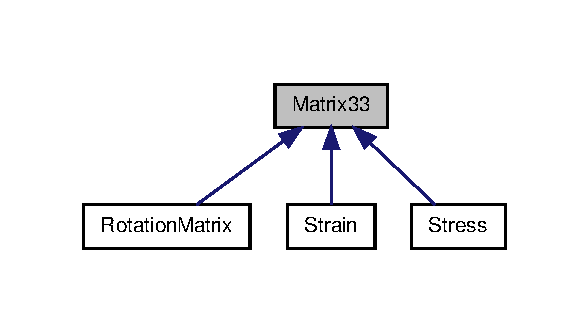
\includegraphics[width=134pt]{dc/dfe/classMatrix33__inherit__graph}
\end{center}
\end{figure}
\subsection*{\-Public \-Member \-Functions}
\begin{DoxyCompactItemize}
\item 
\hyperlink{classMatrix33_a70acb6647b172d017cc4265a29a7d263}{\-Matrix33} ()
\item 
\hyperlink{classMatrix33_a4399c6da8f1ac31ce514550282c823cf}{\-Matrix33} (double $\ast$$\ast$a)
\item 
\hyperlink{classMatrix33_a1f070a29a710043c38b56cee8214e6f7}{\-Matrix33} (\hyperlink{classVector3d}{\-Vector3d} a)
\item 
\hyperlink{classMatrix33_a7f1deae895c26e47c39c76bfaa31d3d2}{\-Matrix33} (\hyperlink{classVector3d}{\-Vector3d} a, \hyperlink{classVector3d}{\-Vector3d} b)
\item 
void \hyperlink{classMatrix33_a6cdcec77fd089b2e73ad7ae85ecff30b}{set\-Value} (int row, int column, double value)
\item 
double \hyperlink{classMatrix33_a849bbdf7b456ddacf7185b087fca4015}{get\-Value} (int row, int column)
\item 
\hyperlink{classMatrix33}{\-Matrix33} \hyperlink{classMatrix33_a4e64ab5af4921c24b8270a0c9050f4ba}{adjugate} ()
\item 
\hyperlink{classMatrix33}{\-Matrix33} \hyperlink{classMatrix33_adc58ec5739c9250ff1150c725d0e868e}{operator+} (const \hyperlink{classMatrix33}{\-Matrix33} \&) const 
\item 
void \hyperlink{classMatrix33_acb59e59d3937e075521f478ba83b7165}{operator+=} (const \hyperlink{classMatrix33}{\-Matrix33} \&)
\item 
\hyperlink{classMatrix33}{\-Matrix33} \hyperlink{classMatrix33_a372f71ec208bb6d3045acd4324b7cb06}{operator-\/} (const \hyperlink{classMatrix33}{\-Matrix33} \&) const 
\item 
void \hyperlink{classMatrix33_abc889e10a9c7c532195c7031c1344a74}{operator-\/=} (const \hyperlink{classMatrix33}{\-Matrix33} \&)
\item 
\hyperlink{classMatrix33}{\-Matrix33} \hyperlink{classMatrix33_a6992fd2bb0b6e9ad71b5d3481c4e3e1a}{operator$\ast$} (const double \&) const 
\item 
void \hyperlink{classMatrix33_a83162791813bef030b1ceb5df3c5cae3}{operator$\ast$=} (const double \&)
\item 
\hyperlink{classMatrix33}{\-Matrix33} \hyperlink{classMatrix33_a525f14614255ff81c0cbab8060e8e065}{operator$\ast$} (const \hyperlink{classMatrix33}{\-Matrix33} \&) const 
\item 
void \hyperlink{classMatrix33_ac3937bdeb034cc83b4adcad16cd58a26}{operator$\ast$=} (const \hyperlink{classMatrix33}{\-Matrix33} \&)
\item 
\hyperlink{classVector3d}{\-Vector3d} \hyperlink{classMatrix33_a601584a1edbaae7c6a2a2874605d6f61}{operator$\ast$} (const \hyperlink{classVector3d}{\-Vector3d} \&) const 
\item 
\hyperlink{classMatrix33}{\-Matrix33} \hyperlink{classMatrix33_ad4ab7b9674a44a297502282e1993ef54}{operator$^\wedge$} () const 
\item 
double \hyperlink{classMatrix33_a15b37caa6ab0d9f4a9f0d95846abd675}{operator$\sim$} () const 
\item 
\hyperlink{classMatrix33}{\-Matrix33} \hyperlink{classMatrix33_a1b822a20343a26b3c9bb7fd5c1247f37}{operator!} () const 
\end{DoxyCompactItemize}
\subsection*{\-Protected \-Attributes}
\begin{DoxyCompactItemize}
\item 
double \hyperlink{classMatrix33_af7f01fa466616eb7c8eda2e4d9f85cdd}{x} \mbox{[}3\mbox{]}\mbox{[}3\mbox{]}
\end{DoxyCompactItemize}


\subsection{\-Detailed \-Description}
\hyperlink{classMatrix33}{\-Matrix33} class representing a 3x3 square matrix. 

\-This class represents a 3x3 square matrix. \-The member functions and operators define various operations that may be carried out on the matrix. 

\-Definition at line 20 of file matrix33.\-h.



\subsection{\-Constructor \& \-Destructor \-Documentation}
\hypertarget{classMatrix33_a70acb6647b172d017cc4265a29a7d263}{\index{\-Matrix33@{\-Matrix33}!\-Matrix33@{\-Matrix33}}
\index{\-Matrix33@{\-Matrix33}!Matrix33@{\-Matrix33}}
\subsubsection[{\-Matrix33}]{\setlength{\rightskip}{0pt plus 5cm}{\bf \-Matrix33\-::\-Matrix33} (
\begin{DoxyParamCaption}
{}
\end{DoxyParamCaption}
)}}\label{de/d82/classMatrix33_a70acb6647b172d017cc4265a29a7d263}
\-Default constructor. 

\-Definition at line 7 of file matrix33.\-cpp.


\begin{DoxyCode}
{
  int i, j;
  
  for (i=0; i<3; i++)
    {
      for (j=0; j<3; j++)
        {
          this->x[i][j] = 0.0;
        }
    }
}
\end{DoxyCode}
\hypertarget{classMatrix33_a4399c6da8f1ac31ce514550282c823cf}{\index{\-Matrix33@{\-Matrix33}!\-Matrix33@{\-Matrix33}}
\index{\-Matrix33@{\-Matrix33}!Matrix33@{\-Matrix33}}
\subsubsection[{\-Matrix33}]{\setlength{\rightskip}{0pt plus 5cm}{\bf \-Matrix33\-::\-Matrix33} (
\begin{DoxyParamCaption}
\item[{double $\ast$$\ast$}]{a}
\end{DoxyParamCaption}
)}}\label{de/d82/classMatrix33_a4399c6da8f1ac31ce514550282c823cf}
\-Constructor with the values provided in a 3x3 matrix. 
\begin{DoxyParams}{\-Parameters}
{\em a} & \-Pointer to the two-\/dimensional 3x3 array. \\
\hline
\end{DoxyParams}


\-Definition at line 24 of file matrix33.\-cpp.


\begin{DoxyCode}
{
  int i, j;
  
  for (i=0; i<3; i++)
    {
      for (j=0; j<3; j++)
        {
          this->x[i][j] = a[i][j];
        }
    }
}
\end{DoxyCode}
\hypertarget{classMatrix33_a1f070a29a710043c38b56cee8214e6f7}{\index{\-Matrix33@{\-Matrix33}!\-Matrix33@{\-Matrix33}}
\index{\-Matrix33@{\-Matrix33}!Matrix33@{\-Matrix33}}
\subsubsection[{\-Matrix33}]{\setlength{\rightskip}{0pt plus 5cm}{\bf \-Matrix33\-::\-Matrix33} (
\begin{DoxyParamCaption}
\item[{{\bf \-Vector3d}}]{a}
\end{DoxyParamCaption}
)}}\label{de/d82/classMatrix33_a1f070a29a710043c38b56cee8214e6f7}
\-Constructor to create the matrix from the dyadic product of a vector with itself. 
\begin{DoxyParams}{\-Parameters}
{\em a} & \-The vector whose dyadic product results in the matrix. \\
\hline
\end{DoxyParams}


\-Definition at line 41 of file matrix33.\-cpp.


\begin{DoxyCode}
{
  int i, j;
  
  for (i=0; i<3; i++)
    {
      for (j=0; j<3; j++)
        {
          this->x[i][j] = a.x[i] * a.x[j];
        }
    }
}
\end{DoxyCode}
\hypertarget{classMatrix33_a7f1deae895c26e47c39c76bfaa31d3d2}{\index{\-Matrix33@{\-Matrix33}!\-Matrix33@{\-Matrix33}}
\index{\-Matrix33@{\-Matrix33}!Matrix33@{\-Matrix33}}
\subsubsection[{\-Matrix33}]{\setlength{\rightskip}{0pt plus 5cm}{\bf \-Matrix33\-::\-Matrix33} (
\begin{DoxyParamCaption}
\item[{{\bf \-Vector3d}}]{a, }
\item[{{\bf \-Vector3d}}]{b}
\end{DoxyParamCaption}
)}}\label{de/d82/classMatrix33_a7f1deae895c26e47c39c76bfaa31d3d2}
\-Constructor with the vectors, the product of which will result in the matrix. 
\begin{DoxyParams}{\-Parameters}
{\em a} & \-First vector. \\
\hline
{\em b} & \-Second vector. \\
\hline
\end{DoxyParams}


\-Definition at line 59 of file matrix33.\-cpp.


\begin{DoxyCode}
{
  int i, j;
  
  for (i=0; i<3; i++)
    {
      for (j=0; j<3; j++)
        {
          this->x[i][j] = a.x[i] * b.x[j];
        }
    }
}
\end{DoxyCode}


\subsection{\-Member \-Function \-Documentation}
\hypertarget{classMatrix33_a4e64ab5af4921c24b8270a0c9050f4ba}{\index{\-Matrix33@{\-Matrix33}!adjugate@{adjugate}}
\index{adjugate@{adjugate}!Matrix33@{\-Matrix33}}
\subsubsection[{adjugate}]{\setlength{\rightskip}{0pt plus 5cm}{\bf \-Matrix33} {\bf \-Matrix33\-::adjugate} (
\begin{DoxyParamCaption}
{}
\end{DoxyParamCaption}
)}}\label{de/d82/classMatrix33_a4e64ab5af4921c24b8270a0c9050f4ba}
\-Returns the adjugate matrix of the present matrix. \begin{DoxyReturn}{\-Returns}
\-The adjugate matrix of the present matrix. 
\end{DoxyReturn}


\-Definition at line 112 of file matrix33.\-cpp.


\begin{DoxyCode}
{
  Matrix33 adj;
  
  adj.x[0][0] = (this->x[1][1]*this->x[2][2]) - (this->x[1][2]*this->x[2][1]);
  adj.x[0][1] = (this->x[1][2]*this->x[2][0]) - (this->x[1][0]*this->x[2][2]);
  adj.x[0][2] = (this->x[1][0]*this->x[2][1]) - (this->x[1][1]*this->x[2][0]);
  
  adj.x[1][0] = (this->x[2][1]*this->x[0][2]) - (this->x[0][1]*this->x[2][2]);
  adj.x[1][1] = (this->x[2][2]*this->x[0][0]) - (this->x[2][0]*this->x[0][2]);
  adj.x[1][2] = (this->x[2][0]*this->x[0][1]) - (this->x[2][1]*this->x[0][0]);
  
  adj.x[2][0] = (this->x[0][1]*this->x[1][2]) - (this->x[0][2]*this->x[1][1]);
  adj.x[2][1] = (this->x[0][2]*this->x[1][0]) - (this->x[0][0]*this->x[1][2]);
  adj.x[2][2] = (this->x[0][0]*this->x[1][1]) - (this->x[1][0]*this->x[0][1]);

  return (adj);
}
\end{DoxyCode}
\hypertarget{classMatrix33_a849bbdf7b456ddacf7185b087fca4015}{\index{\-Matrix33@{\-Matrix33}!get\-Value@{get\-Value}}
\index{get\-Value@{get\-Value}!Matrix33@{\-Matrix33}}
\subsubsection[{get\-Value}]{\setlength{\rightskip}{0pt plus 5cm}double {\bf \-Matrix33\-::get\-Value} (
\begin{DoxyParamCaption}
\item[{int}]{row, }
\item[{int}]{column}
\end{DoxyParamCaption}
)}}\label{de/d82/classMatrix33_a849bbdf7b456ddacf7185b087fca4015}
\-Returns the value of the element located by the row and column indices provided. 
\begin{DoxyParams}{\-Parameters}
{\em row} & \-Row index of the element. \\
\hline
{\em column} & \-Column index of the element. \\
\hline
\end{DoxyParams}
\begin{DoxyReturn}{\-Returns}
\-Value of the element located at the given position.
\end{DoxyReturn}
\-Returns the value of the element located by the row and column indices provided. 
\begin{DoxyParams}{\-Parameters}
{\em row} & \-Row index of the element. \\
\hline
{\em column} & \-Column index of the element. \\
\hline
\end{DoxyParams}


\-Definition at line 95 of file matrix33.\-cpp.


\begin{DoxyCode}
{
  if (row>=0 && row<3)
    {
      if (column>=0 && column<3)
        {
          return (this->x[row][column]);
        }
    }
  
  return (0.0);
}
\end{DoxyCode}
\hypertarget{classMatrix33_a1b822a20343a26b3c9bb7fd5c1247f37}{\index{\-Matrix33@{\-Matrix33}!operator!@{operator!}}
\index{operator!@{operator!}!Matrix33@{\-Matrix33}}
\subsubsection[{operator!}]{\setlength{\rightskip}{0pt plus 5cm}{\bf \-Matrix33} {\bf \-Matrix33\-::operator!} (
\begin{DoxyParamCaption}
{}
\end{DoxyParamCaption}
) const}}\label{de/d82/classMatrix33_a1b822a20343a26b3c9bb7fd5c1247f37}
\-Returns in a new matrix the inverse of the current matrix. \-If the current matrix is non-\/invertible, a zero matrix is returned. 

\-Definition at line 342 of file matrix33.\-cpp.


\begin{DoxyCode}
{
  Matrix33 r;   // Result matrix
  
  double determinant = ~(*this);
  
  if (determinant == 0.0)
    {
      // The matrix is non-invertible
      return (r);       // Zero matrix
    }
  
  // If we are still here, the matrix is invertible
  
  //  Transpose
  Matrix33 tr = ^(*this);
  
  // Find Adjugate matrix
  Matrix33 adj = tr.adjugate();
  
  // Calculate the inverse by dividing the adjugate matrix by the determinant
  r = adj * (1.0/determinant);
  
  return (r);
}
\end{DoxyCode}
\hypertarget{classMatrix33_a6992fd2bb0b6e9ad71b5d3481c4e3e1a}{\index{\-Matrix33@{\-Matrix33}!operator$\ast$@{operator$\ast$}}
\index{operator$\ast$@{operator$\ast$}!Matrix33@{\-Matrix33}}
\subsubsection[{operator$\ast$}]{\setlength{\rightskip}{0pt plus 5cm}{\bf \-Matrix33} \-Matrix33\-::operator$\ast$ (
\begin{DoxyParamCaption}
\item[{const double \&}]{p}
\end{DoxyParamCaption}
) const}}\label{de/d82/classMatrix33_a6992fd2bb0b6e9ad71b5d3481c4e3e1a}
\-Operator for scaling the matrix by a scalar. \-Scales the current matrix by the scalar provided and returns the result in a third matrix. 

\-Definition at line 213 of file matrix33.\-cpp.


\begin{DoxyCode}
{
  int i, j;
  Matrix33 r;
  
  for (i=0; i<3; i++)
    {
      for (j=0; j<3; j++)
        {
          r.x[i][j] = this->x[i][j] * p;
        }
    }
  
  return (r);
}
\end{DoxyCode}
\hypertarget{classMatrix33_a525f14614255ff81c0cbab8060e8e065}{\index{\-Matrix33@{\-Matrix33}!operator$\ast$@{operator$\ast$}}
\index{operator$\ast$@{operator$\ast$}!Matrix33@{\-Matrix33}}
\subsubsection[{operator$\ast$}]{\setlength{\rightskip}{0pt plus 5cm}{\bf \-Matrix33} \-Matrix33\-::operator$\ast$ (
\begin{DoxyParamCaption}
\item[{const {\bf \-Matrix33} \&}]{p}
\end{DoxyParamCaption}
) const}}\label{de/d82/classMatrix33_a525f14614255ff81c0cbab8060e8e065}
\-Operator for the multiplication of two matrices. \-Multiplies the current matrix with another 3x3 matrix and returns the result in a new matrix. 

\-Definition at line 250 of file matrix33.\-cpp.


\begin{DoxyCode}
{
  int i, j, k;
  Matrix33 r;
  
  for (i=0; i<3; i++)
    {
      for (j=0; j<3; j++)
        {
          r.x[i][j] = 0.0;
          for (k=0; k<3; k++)
            {
              r.x[i][j] += this->x[i][k] * p.x[k][j];
            }
        }
    }
  
  return (r);
}
\end{DoxyCode}
\hypertarget{classMatrix33_a601584a1edbaae7c6a2a2874605d6f61}{\index{\-Matrix33@{\-Matrix33}!operator$\ast$@{operator$\ast$}}
\index{operator$\ast$@{operator$\ast$}!Matrix33@{\-Matrix33}}
\subsubsection[{operator$\ast$}]{\setlength{\rightskip}{0pt plus 5cm}{\bf \-Vector3d} \-Matrix33\-::operator$\ast$ (
\begin{DoxyParamCaption}
\item[{const {\bf \-Vector3d} \&}]{v}
\end{DoxyParamCaption}
) const}}\label{de/d82/classMatrix33_a601584a1edbaae7c6a2a2874605d6f61}
\-Returns in a vector the result of the multiplication of the current matrix with the provided vector. 

\-Definition at line 288 of file matrix33.\-cpp.


\begin{DoxyCode}
{
  Vector3d r(0.0, 0.0, 0.0);
  int i, j;
  
  for (i=0; i<3; i++)
    {
      for (j=0; j<3; j++)
        {
          r[i] += this->x[i][j] * v.x[j];
        }
    }
  
  return (r);
}
\end{DoxyCode}
\hypertarget{classMatrix33_a83162791813bef030b1ceb5df3c5cae3}{\index{\-Matrix33@{\-Matrix33}!operator$\ast$=@{operator$\ast$=}}
\index{operator$\ast$=@{operator$\ast$=}!Matrix33@{\-Matrix33}}
\subsubsection[{operator$\ast$=}]{\setlength{\rightskip}{0pt plus 5cm}void \-Matrix33\-::operator$\ast$= (
\begin{DoxyParamCaption}
\item[{const double \&}]{p}
\end{DoxyParamCaption}
)}}\label{de/d82/classMatrix33_a83162791813bef030b1ceb5df3c5cae3}
\-Operator for reflexive scaling of the matrix by a scalar. \-Scales the current matrix by the scalar provided and populates the current matrix elements with the result. 

\-Definition at line 233 of file matrix33.\-cpp.


\begin{DoxyCode}
{
  int i, j;
  
  for (i=0; i<3; i++)
    {
      for (j=0; j<3; j++)
        {
          this->x[i][j] *= p;
        }
    }
}
\end{DoxyCode}
\hypertarget{classMatrix33_ac3937bdeb034cc83b4adcad16cd58a26}{\index{\-Matrix33@{\-Matrix33}!operator$\ast$=@{operator$\ast$=}}
\index{operator$\ast$=@{operator$\ast$=}!Matrix33@{\-Matrix33}}
\subsubsection[{operator$\ast$=}]{\setlength{\rightskip}{0pt plus 5cm}void \-Matrix33\-::operator$\ast$= (
\begin{DoxyParamCaption}
\item[{const {\bf \-Matrix33} \&}]{p}
\end{DoxyParamCaption}
)}}\label{de/d82/classMatrix33_ac3937bdeb034cc83b4adcad16cd58a26}
\-Operator for reflexive multiplication of two matrices. \-Multiplies the current matrix with another 3x3 matrix and populates the elements of the current matrix with the result. 

\-Definition at line 274 of file matrix33.\-cpp.


\begin{DoxyCode}
{
  Matrix33* r = new Matrix33;
  
  *r = (*this) * p;
  *this = *r;
  
  delete(r);
  r = NULL;
}
\end{DoxyCode}
\hypertarget{classMatrix33_adc58ec5739c9250ff1150c725d0e868e}{\index{\-Matrix33@{\-Matrix33}!operator+@{operator+}}
\index{operator+@{operator+}!Matrix33@{\-Matrix33}}
\subsubsection[{operator+}]{\setlength{\rightskip}{0pt plus 5cm}{\bf \-Matrix33} \-Matrix33\-::operator+ (
\begin{DoxyParamCaption}
\item[{const {\bf \-Matrix33} \&}]{p}
\end{DoxyParamCaption}
) const}}\label{de/d82/classMatrix33_adc58ec5739c9250ff1150c725d0e868e}
\-Operator for addition of two matrices. \-Adds the current matrix to the provided matrix and returns a third matrix with the result. 

\-Definition at line 137 of file matrix33.\-cpp.


\begin{DoxyCode}
{
  int i, j;
  Matrix33 r;
  
  for (i=0; i<3; i++)
    {
      for (j=0; j<3; j++)
        {
          r.x[i][j] = this->x[i][j] + p.x[i][j];
        }
    }
  
  return (r);
}
\end{DoxyCode}
\hypertarget{classMatrix33_acb59e59d3937e075521f478ba83b7165}{\index{\-Matrix33@{\-Matrix33}!operator+=@{operator+=}}
\index{operator+=@{operator+=}!Matrix33@{\-Matrix33}}
\subsubsection[{operator+=}]{\setlength{\rightskip}{0pt plus 5cm}void \-Matrix33\-::operator+= (
\begin{DoxyParamCaption}
\item[{const {\bf \-Matrix33} \&}]{p}
\end{DoxyParamCaption}
)}}\label{de/d82/classMatrix33_acb59e59d3937e075521f478ba83b7165}
\-Operator for reflexive addition of two matrices. \-Adds the current matrix to the provided matrix and populates the current matrix elements with the result. 

\-Definition at line 157 of file matrix33.\-cpp.


\begin{DoxyCode}
{
  int i, j;
  
  for (i=0; i<3; i++)
    {
      for (j=0; j<3; j++)
        {
          this->x[i][j] += p.x[i][j];
        }
    }
}
\end{DoxyCode}
\hypertarget{classMatrix33_a372f71ec208bb6d3045acd4324b7cb06}{\index{\-Matrix33@{\-Matrix33}!operator-\/@{operator-\/}}
\index{operator-\/@{operator-\/}!Matrix33@{\-Matrix33}}
\subsubsection[{operator-\/}]{\setlength{\rightskip}{0pt plus 5cm}{\bf \-Matrix33} \-Matrix33\-::operator-\/ (
\begin{DoxyParamCaption}
\item[{const {\bf \-Matrix33} \&}]{p}
\end{DoxyParamCaption}
) const}}\label{de/d82/classMatrix33_a372f71ec208bb6d3045acd4324b7cb06}
\-Operator for the subtraction of two matrices. \-Subtracts the given matrix from the current matrix and returns the result in a new matrix. 

\-Definition at line 175 of file matrix33.\-cpp.


\begin{DoxyCode}
{
  int i, j;
  Matrix33 r;
  
  for (i=0; i<3; i++)
    {
      for (j=0; j<3; j++)
        {
          r.x[i][j] = this->x[i][j] - p.x[i][j];
        }
    }
  
  return (r);
}
\end{DoxyCode}
\hypertarget{classMatrix33_abc889e10a9c7c532195c7031c1344a74}{\index{\-Matrix33@{\-Matrix33}!operator-\/=@{operator-\/=}}
\index{operator-\/=@{operator-\/=}!Matrix33@{\-Matrix33}}
\subsubsection[{operator-\/=}]{\setlength{\rightskip}{0pt plus 5cm}void \-Matrix33\-::operator-\/= (
\begin{DoxyParamCaption}
\item[{const {\bf \-Matrix33} \&}]{p}
\end{DoxyParamCaption}
)}}\label{de/d82/classMatrix33_abc889e10a9c7c532195c7031c1344a74}
\-Operator for reflexive subtraction of two matrices. \-Subtracts the given matrix from the current matrix and populates the current matrix with the result. 

\-Definition at line 195 of file matrix33.\-cpp.


\begin{DoxyCode}
{
  int i, j;
  
  for (i=0; i<3; i++)
    {
      for (j=0; j<3; j++)
        {
          this->x[i][j] -= p.x[i][j];
        }
    }
}
\end{DoxyCode}
\hypertarget{classMatrix33_ad4ab7b9674a44a297502282e1993ef54}{\index{\-Matrix33@{\-Matrix33}!operator$^\wedge$@{operator$^\wedge$}}
\index{operator$^\wedge$@{operator$^\wedge$}!Matrix33@{\-Matrix33}}
\subsubsection[{operator$^\wedge$}]{\setlength{\rightskip}{0pt plus 5cm}{\bf \-Matrix33} \-Matrix33\-::operator$^\wedge$ (
\begin{DoxyParamCaption}
{}
\end{DoxyParamCaption}
) const}}\label{de/d82/classMatrix33_ad4ab7b9674a44a297502282e1993ef54}
\-Returns in a new matrix the transpose of the current matrix. 

\-Definition at line 308 of file matrix33.\-cpp.


\begin{DoxyCode}
{
  Matrix33 r;
  int i, j;
  
  for (i=0; i<3; i++)
    {
      for (j=0; j<3; j++)
        {
          r.x[i][j] = this->x[j][i];
        }
    }
  
  return (r);
}
\end{DoxyCode}
\hypertarget{classMatrix33_a15b37caa6ab0d9f4a9f0d95846abd675}{\index{\-Matrix33@{\-Matrix33}!operator$\sim$@{operator$\sim$}}
\index{operator$\sim$@{operator$\sim$}!Matrix33@{\-Matrix33}}
\subsubsection[{operator$\sim$}]{\setlength{\rightskip}{0pt plus 5cm}double {\bf \-Matrix33\-::operator$\sim$} (
\begin{DoxyParamCaption}
{}
\end{DoxyParamCaption}
) const}}\label{de/d82/classMatrix33_a15b37caa6ab0d9f4a9f0d95846abd675}
\-Returns the determinant of the current matrix. 

\-Definition at line 327 of file matrix33.\-cpp.


\begin{DoxyCode}
{
  double d = 0.0;
  
  d += this.x[0][0] * ( (this->x[1][1]*this->x[2][2]) - (this->x[2][1]*this->x[
      1][2]) );
  d += this.x[0][1] * ( (this->x[1][2]*this->x[2][0]) - (this->x[1][0]*this->x[
      2][2]) );
  d += this.x[0][2] * ( (this->x[1][0]*this->x[2][1]) - (this->x[2][0]*this->x[
      1][1]) );
  
  return (d);
}
\end{DoxyCode}
\hypertarget{classMatrix33_a6cdcec77fd089b2e73ad7ae85ecff30b}{\index{\-Matrix33@{\-Matrix33}!set\-Value@{set\-Value}}
\index{set\-Value@{set\-Value}!Matrix33@{\-Matrix33}}
\subsubsection[{set\-Value}]{\setlength{\rightskip}{0pt plus 5cm}void {\bf \-Matrix33\-::set\-Value} (
\begin{DoxyParamCaption}
\item[{int}]{row, }
\item[{int}]{column, }
\item[{double}]{value}
\end{DoxyParamCaption}
)}}\label{de/d82/classMatrix33_a6cdcec77fd089b2e73ad7ae85ecff30b}
\-Function to set the value of an element indicated by its position. 
\begin{DoxyParams}{\-Parameters}
{\em row} & \-Row index of the element. \\
\hline
{\em column} & \-Column index of the element. \\
\hline
{\em value} & \-Value that the element is to be set to. \\
\hline
\end{DoxyParams}


\-Definition at line 79 of file matrix33.\-cpp.


\begin{DoxyCode}
{
  if (row>=0 && row<3)
    {
      if (column>=0 && column<3)
        {
          this->x[row][column] = value;
        }
    }
}
\end{DoxyCode}


\subsection{\-Field \-Documentation}
\hypertarget{classMatrix33_af7f01fa466616eb7c8eda2e4d9f85cdd}{\index{\-Matrix33@{\-Matrix33}!x@{x}}
\index{x@{x}!Matrix33@{\-Matrix33}}
\subsubsection[{x}]{\setlength{\rightskip}{0pt plus 5cm}double {\bf \-Matrix33\-::x}\mbox{[}3\mbox{]}\mbox{[}3\mbox{]}\hspace{0.3cm}{\ttfamily  \mbox{[}protected\mbox{]}}}}\label{de/d82/classMatrix33_af7f01fa466616eb7c8eda2e4d9f85cdd}
\-Array containing the elements of the matrix. 

\-Definition at line 26 of file matrix33.\-h.



\-The documentation for this class was generated from the following files\-:\begin{DoxyCompactItemize}
\item 
\hyperlink{matrix33_8h}{matrix33.\-h}\item 
\hyperlink{matrix33_8cpp}{matrix33.\-cpp}\end{DoxyCompactItemize}

\hypertarget{classRotationMatrix}{\section{Rotation\-Matrix Class Reference}
\label{d2/d4a/classRotationMatrix}\index{Rotation\-Matrix@{Rotation\-Matrix}}
}


\hyperlink{classRotationMatrix}{Rotation\-Matrix} class to represent a rotation matrix.  




{\ttfamily \#include $<$rotation\-Matrix.\-h$>$}



Inheritance diagram for Rotation\-Matrix\-:\nopagebreak
\begin{figure}[H]
\begin{center}
\leavevmode
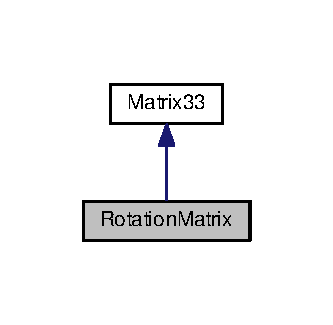
\includegraphics[width=160pt]{d5/d4d/classRotationMatrix__inherit__graph}
\end{center}
\end{figure}


Collaboration diagram for Rotation\-Matrix\-:\nopagebreak
\begin{figure}[H]
\begin{center}
\leavevmode
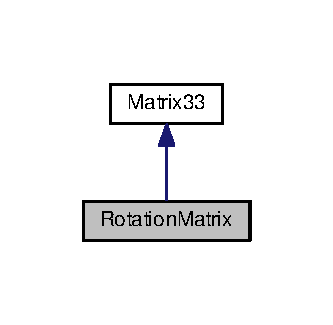
\includegraphics[width=160pt]{d5/dc0/classRotationMatrix__coll__graph}
\end{center}
\end{figure}
\subsection*{Public Member Functions}
\begin{DoxyCompactItemize}
\item 
\hyperlink{classRotationMatrix_a4678658c45a6b89f2d06c48b318e2769}{Rotation\-Matrix} ()
\begin{DoxyCompactList}\small\item\em Default constructor. \end{DoxyCompactList}\item 
\hyperlink{classRotationMatrix_a234bf349cf56fc8561a41f5a3669675b}{Rotation\-Matrix} (\hyperlink{classMatrix33}{Matrix33} m)
\begin{DoxyCompactList}\small\item\em Constructor specifying the matrix. \end{DoxyCompactList}\item 
\hyperlink{classRotationMatrix_aa5506a5341c05e42d258a93137635a9b}{Rotation\-Matrix} (\hyperlink{classVector3d}{Vector3d} $\ast$un\-Primed, \hyperlink{classVector3d}{Vector3d} $\ast$primed)
\begin{DoxyCompactList}\small\item\em Defines the rotation matrix based on two co-\/ordinate systems. \end{DoxyCompactList}\item 
void \hyperlink{classMatrix33_a6cdcec77fd089b2e73ad7ae85ecff30b}{set\-Value} (int row, int column, double value)
\begin{DoxyCompactList}\small\item\em Function to set the value of an element indicated by its position. \end{DoxyCompactList}\item 
double \hyperlink{classMatrix33_ab53b3e37ad830a87a804cf26311ba088}{get\-Value} (int row, int column) const 
\begin{DoxyCompactList}\small\item\em Returns the value of the element located by the row and column indices provided. \end{DoxyCompactList}\item 
\hyperlink{classMatrix33}{Matrix33} \hyperlink{classMatrix33_a07b999a7b1c905f3c98ba3792e6fa33f}{adjugate} () const 
\begin{DoxyCompactList}\small\item\em Returns the adjugate matrix of the present matrix. \end{DoxyCompactList}\item 
\hyperlink{classMatrix33}{Matrix33} \hyperlink{classMatrix33_a64418c1a8836b38526fdfd7ffcc79cfd}{transpose} () const 
\begin{DoxyCompactList}\small\item\em Returns the transpose of the present matrix. \end{DoxyCompactList}\item 
\hyperlink{classMatrix33}{Matrix33} \hyperlink{classMatrix33_adc58ec5739c9250ff1150c725d0e868e}{operator+} (const \hyperlink{classMatrix33}{Matrix33} \&) const 
\begin{DoxyCompactList}\small\item\em Operator for addition of two matrices. \end{DoxyCompactList}\item 
void \hyperlink{classMatrix33_acb59e59d3937e075521f478ba83b7165}{operator+=} (const \hyperlink{classMatrix33}{Matrix33} \&)
\begin{DoxyCompactList}\small\item\em Operator for reflexive addition of two matrices. \end{DoxyCompactList}\item 
\hyperlink{classMatrix33}{Matrix33} \hyperlink{classMatrix33_a372f71ec208bb6d3045acd4324b7cb06}{operator-\/} (const \hyperlink{classMatrix33}{Matrix33} \&) const 
\begin{DoxyCompactList}\small\item\em Operator for the subtraction of two matrices. \end{DoxyCompactList}\item 
void \hyperlink{classMatrix33_abc889e10a9c7c532195c7031c1344a74}{operator-\/=} (const \hyperlink{classMatrix33}{Matrix33} \&)
\begin{DoxyCompactList}\small\item\em Operator for reflexive subtraction of two matrices. \end{DoxyCompactList}\item 
\hyperlink{classMatrix33}{Matrix33} \hyperlink{classMatrix33_a6992fd2bb0b6e9ad71b5d3481c4e3e1a}{operator$\ast$} (const double \&) const 
\begin{DoxyCompactList}\small\item\em Operator for scaling the matrix by a scalar. \end{DoxyCompactList}\item 
\hyperlink{classMatrix33}{Matrix33} \hyperlink{classMatrix33_a525f14614255ff81c0cbab8060e8e065}{operator$\ast$} (const \hyperlink{classMatrix33}{Matrix33} \&) const 
\begin{DoxyCompactList}\small\item\em Operator for the multiplication of two matrices. \end{DoxyCompactList}\item 
\hyperlink{classVector3d}{Vector3d} \hyperlink{classMatrix33_a601584a1edbaae7c6a2a2874605d6f61}{operator$\ast$} (const \hyperlink{classVector3d}{Vector3d} \&) const 
\begin{DoxyCompactList}\small\item\em Operator for the multiplication of a matrix with a vector. \end{DoxyCompactList}\item 
void \hyperlink{classMatrix33_a83162791813bef030b1ceb5df3c5cae3}{operator$\ast$=} (const double \&)
\begin{DoxyCompactList}\small\item\em Operator for reflexive scaling of the matrix by a scalar. \end{DoxyCompactList}\item 
void \hyperlink{classMatrix33_ac3937bdeb034cc83b4adcad16cd58a26}{operator$\ast$=} (const \hyperlink{classMatrix33}{Matrix33} \&)
\begin{DoxyCompactList}\small\item\em Operator for reflexive multiplication of two matrices. \end{DoxyCompactList}\item 
double \hyperlink{classMatrix33_a15b37caa6ab0d9f4a9f0d95846abd675}{operator$\sim$} () const 
\begin{DoxyCompactList}\small\item\em Determinant. \end{DoxyCompactList}\item 
\hyperlink{classMatrix33}{Matrix33} \hyperlink{classMatrix33_a1b822a20343a26b3c9bb7fd5c1247f37}{operator!} () const 
\begin{DoxyCompactList}\small\item\em Inverse. \end{DoxyCompactList}\end{DoxyCompactItemize}
\subsection*{Protected Attributes}
\begin{DoxyCompactItemize}
\item 
double \hyperlink{classMatrix33_af7f01fa466616eb7c8eda2e4d9f85cdd}{x} \mbox{[}3\mbox{]}\mbox{[}3\mbox{]}
\begin{DoxyCompactList}\small\item\em Array containing the elements of the matrix. \end{DoxyCompactList}\end{DoxyCompactItemize}


\subsection{Detailed Description}
\hyperlink{classRotationMatrix}{Rotation\-Matrix} class to represent a rotation matrix. 

The member functions of this class create a rotation matrix for carrying out rotations in 3\-D and transformation of axes. 

Definition at line 19 of file rotation\-Matrix.\-h.



\subsection{Constructor \& Destructor Documentation}
\hypertarget{classRotationMatrix_a4678658c45a6b89f2d06c48b318e2769}{\index{Rotation\-Matrix@{Rotation\-Matrix}!Rotation\-Matrix@{Rotation\-Matrix}}
\index{Rotation\-Matrix@{Rotation\-Matrix}!RotationMatrix@{Rotation\-Matrix}}
\subsubsection[{Rotation\-Matrix}]{\setlength{\rightskip}{0pt plus 5cm}Rotation\-Matrix\-::\-Rotation\-Matrix (
\begin{DoxyParamCaption}
{}
\end{DoxyParamCaption}
)}}\label{d2/d4a/classRotationMatrix_a4678658c45a6b89f2d06c48b318e2769}


Default constructor. 

Initializes the rotation matrix with a unit matrix. 

Definition at line 16 of file rotation\-Matrix.\-cpp.


\begin{DoxyCode}
17 \{
18     \textcolor{keywordtype}{int} i,  j;
19 
20     \textcolor{keywordflow}{for} ( i=0; i<3; i++ ) \{
21         \textcolor{keywordflow}{for} ( j=0; i<3; j++ ) \{
22             \textcolor{keywordflow}{if} ( i==j ) \{
23                 this->\hyperlink{classMatrix33_a6cdcec77fd089b2e73ad7ae85ecff30b}{setValue} ( i, j, 1.0 );
24             \}
25             \textcolor{keywordflow}{else} \{
26                 this->\hyperlink{classMatrix33_a6cdcec77fd089b2e73ad7ae85ecff30b}{setValue} ( i, j, 0.0 );
27             \}
28         \}
29     \}
30 \}
\end{DoxyCode}
\hypertarget{classRotationMatrix_a234bf349cf56fc8561a41f5a3669675b}{\index{Rotation\-Matrix@{Rotation\-Matrix}!Rotation\-Matrix@{Rotation\-Matrix}}
\index{Rotation\-Matrix@{Rotation\-Matrix}!RotationMatrix@{Rotation\-Matrix}}
\subsubsection[{Rotation\-Matrix}]{\setlength{\rightskip}{0pt plus 5cm}Rotation\-Matrix\-::\-Rotation\-Matrix (
\begin{DoxyParamCaption}
\item[{{\bf Matrix33}}]{m}
\end{DoxyParamCaption}
)}}\label{d2/d4a/classRotationMatrix_a234bf349cf56fc8561a41f5a3669675b}


Constructor specifying the matrix. 

The rotation matrix is provided as the matrix m. 
\begin{DoxyParams}{Parameters}
{\em m} & The matrix m which is equal to the rotation matrix. \\
\hline
\end{DoxyParams}


Definition at line 37 of file rotation\-Matrix.\-cpp.


\begin{DoxyCode}
38 \{
39   \textcolor{keywordtype}{int} i, j;
40 
41   \textcolor{keywordflow}{for} (i=0; i<3; i++)
42     \{
43       \textcolor{keywordflow}{for} (j=0; j<3; j++)
44         \{
45           this->\hyperlink{classMatrix33_a6cdcec77fd089b2e73ad7ae85ecff30b}{setValue} (i, j, (m.\hyperlink{classMatrix33_ab53b3e37ad830a87a804cf26311ba088}{getValue}(i,j)));
46         \}
47     \}
48 \}
\end{DoxyCode}
\hypertarget{classRotationMatrix_aa5506a5341c05e42d258a93137635a9b}{\index{Rotation\-Matrix@{Rotation\-Matrix}!Rotation\-Matrix@{Rotation\-Matrix}}
\index{Rotation\-Matrix@{Rotation\-Matrix}!RotationMatrix@{Rotation\-Matrix}}
\subsubsection[{Rotation\-Matrix}]{\setlength{\rightskip}{0pt plus 5cm}Rotation\-Matrix\-::\-Rotation\-Matrix (
\begin{DoxyParamCaption}
\item[{{\bf Vector3d} $\ast$}]{un\-Primed, }
\item[{{\bf Vector3d} $\ast$}]{primed}
\end{DoxyParamCaption}
)}}\label{d2/d4a/classRotationMatrix_aa5506a5341c05e42d258a93137635a9b}


Defines the rotation matrix based on two co-\/ordinate systems. 

The rotation matrix is created using the axes of the two co-\/ordinate systems provided as arguments. The vectors must be normalized to be unit vectors. 
\begin{DoxyParams}{Parameters}
{\em un\-Primed} & Pointer to the array containing the three axes vectors of the unprimed (old) system. \\
\hline
{\em primed} & Pointer to the array containing the three axes vectors of the primed (new) system. \\
\hline
\end{DoxyParams}


Definition at line 56 of file rotation\-Matrix.\-cpp.


\begin{DoxyCode}
57 \{
58     \textcolor{keywordtype}{int} i, j;
59 
60     \textcolor{keywordflow}{for} ( i=0; i<3; i++ ) \{
61         \textcolor{keywordflow}{for} ( j=0; j<3; j++ ) \{
62             this->\hyperlink{classMatrix33_a6cdcec77fd089b2e73ad7ae85ecff30b}{setValue} ( i, j, primed[i]*unPrimed[j] );
63         \}
64     \}
65 \}
\end{DoxyCode}


\subsection{Member Function Documentation}
\hypertarget{classMatrix33_a07b999a7b1c905f3c98ba3792e6fa33f}{\index{Rotation\-Matrix@{Rotation\-Matrix}!adjugate@{adjugate}}
\index{adjugate@{adjugate}!RotationMatrix@{Rotation\-Matrix}}
\subsubsection[{adjugate}]{\setlength{\rightskip}{0pt plus 5cm}{\bf Matrix33} Matrix33\-::adjugate (
\begin{DoxyParamCaption}
{}
\end{DoxyParamCaption}
) const\hspace{0.3cm}{\ttfamily [inherited]}}}\label{de/d82/classMatrix33_a07b999a7b1c905f3c98ba3792e6fa33f}


Returns the adjugate matrix of the present matrix. 

The adjugate matrix of the present matrix is returned. The adjugate matrix is calculated by evaluating the determinant of the cofactor matrix of each element, and then replacing the corresponding element position by the value of the determinant. This operation is useful in calculating the inverse of a matrix. \begin{DoxyReturn}{Returns}
The adjugate matrix of the present matrix. 
\end{DoxyReturn}


Definition at line 129 of file matrix33.\-cpp.


\begin{DoxyCode}
130 \{
131   \hyperlink{classMatrix33}{Matrix33} adj;
132   
133   adj.\hyperlink{classMatrix33_a6cdcec77fd089b2e73ad7ae85ecff30b}{setValue}(0, 0, ((this->\hyperlink{classMatrix33_af7f01fa466616eb7c8eda2e4d9f85cdd}{x}[1][1]*this->\hyperlink{classMatrix33_af7f01fa466616eb7c8eda2e4d9f85cdd}{x}[2][2]) - (this->x[1][2]*this->x[2][1])));
134   adj.\hyperlink{classMatrix33_a6cdcec77fd089b2e73ad7ae85ecff30b}{setValue}(0, 1, ((this->x[1][2]*this->x[2][0]) - (this->x[1][0]*this->x[2][2])));
135   adj.\hyperlink{classMatrix33_a6cdcec77fd089b2e73ad7ae85ecff30b}{setValue}(0, 2, ((this->x[1][0]*this->x[2][1]) - (this->x[1][1]*this->x[2][0])));
136   
137   adj.\hyperlink{classMatrix33_a6cdcec77fd089b2e73ad7ae85ecff30b}{setValue}(1, 0, ((this->x[2][1]*this->x[0][2]) - (this->x[0][1]*this->x[2][2])));
138   adj.\hyperlink{classMatrix33_a6cdcec77fd089b2e73ad7ae85ecff30b}{setValue}(1, 1, ((this->x[2][2]*this->x[0][0]) - (this->x[2][0]*this->x[0][2])));
139   adj.\hyperlink{classMatrix33_a6cdcec77fd089b2e73ad7ae85ecff30b}{setValue}(1, 2, ((this->x[2][0]*this->x[0][1]) - (this->x[2][1]*this->x[0][0])));
140   
141   adj.\hyperlink{classMatrix33_a6cdcec77fd089b2e73ad7ae85ecff30b}{setValue}(2, 0, ((this->x[0][1]*this->x[1][2]) - (this->x[0][2]*this->x[1][1])));
142   adj.\hyperlink{classMatrix33_a6cdcec77fd089b2e73ad7ae85ecff30b}{setValue}(2, 1, ((this->x[0][2]*this->x[1][0]) - (this->x[0][0]*this->x[1][2])));
143   adj.\hyperlink{classMatrix33_a6cdcec77fd089b2e73ad7ae85ecff30b}{setValue}(2, 2, ((this->x[0][0]*this->x[1][1]) - (this->x[1][0]*this->x[0][1])));
144 
145   \textcolor{keywordflow}{return} (adj);
146 \}
\end{DoxyCode}
\hypertarget{classMatrix33_ab53b3e37ad830a87a804cf26311ba088}{\index{Rotation\-Matrix@{Rotation\-Matrix}!get\-Value@{get\-Value}}
\index{get\-Value@{get\-Value}!RotationMatrix@{Rotation\-Matrix}}
\subsubsection[{get\-Value}]{\setlength{\rightskip}{0pt plus 5cm}double Matrix33\-::get\-Value (
\begin{DoxyParamCaption}
\item[{int}]{row, }
\item[{int}]{column}
\end{DoxyParamCaption}
) const\hspace{0.3cm}{\ttfamily [inherited]}}}\label{de/d82/classMatrix33_ab53b3e37ad830a87a804cf26311ba088}


Returns the value of the element located by the row and column indices provided. 

The value of the element indicated by the arguments row and column is returned. The values of row and column must correspond to array indices, and thus can be one of 0, 1 and 2. In any other case 0.\-0 is returned. 
\begin{DoxyParams}{Parameters}
{\em row} & Row index of the element. \\
\hline
{\em column} & Column index of the element. \\
\hline
\end{DoxyParams}
\begin{DoxyReturn}{Returns}
Value of the element located at the given position. 
\end{DoxyReturn}


Definition at line 111 of file matrix33.\-cpp.


\begin{DoxyCode}
112 \{
113   \textcolor{keywordflow}{if} (row>=0 && row<3)
114     \{
115       \textcolor{keywordflow}{if} (column>=0 && column<3)
116         \{
117           \textcolor{keywordflow}{return} (this->\hyperlink{classMatrix33_af7f01fa466616eb7c8eda2e4d9f85cdd}{x}[row][column]);
118         \}
119     \}
120   
121   \textcolor{keywordflow}{return} (0.0);
122 \}
\end{DoxyCode}
\hypertarget{classMatrix33_a1b822a20343a26b3c9bb7fd5c1247f37}{\index{Rotation\-Matrix@{Rotation\-Matrix}!operator!@{operator!}}
\index{operator!@{operator!}!RotationMatrix@{Rotation\-Matrix}}
\subsubsection[{operator!}]{\setlength{\rightskip}{0pt plus 5cm}{\bf Matrix33} Matrix33\-::operator! (
\begin{DoxyParamCaption}
{}
\end{DoxyParamCaption}
) const\hspace{0.3cm}{\ttfamily [inherited]}}}\label{de/d82/classMatrix33_a1b822a20343a26b3c9bb7fd5c1247f37}


Inverse. 

Returns in a new matrix the inverse of the current matrix. If the current matrix is non-\/invertible, a zero matrix is returned. \begin{DoxyReturn}{Returns}
Matrix with the inverse of the current matrix. If the current matrix is non-\/invertible, a zero matrix is returned. 
\end{DoxyReturn}


Definition at line 374 of file matrix33.\-cpp.


\begin{DoxyCode}
375 \{
376   \hyperlink{classMatrix33}{Matrix33} r;   \textcolor{comment}{// Result matrix}
377   
378   \textcolor{keywordtype}{double} determinant = ~(*this);
379   
380   \textcolor{keywordflow}{if} (determinant == 0.0)
381     \{
382       \textcolor{comment}{// The matrix is non-invertible}
383       \textcolor{keywordflow}{return} (r);       \textcolor{comment}{// Zero matrix}
384     \}
385   
386   \textcolor{comment}{// If we are still here, the matrix is invertible}
387   
388   \textcolor{comment}{//  Transpose}
389   \hyperlink{classMatrix33}{Matrix33} tr = this->\hyperlink{classMatrix33_a64418c1a8836b38526fdfd7ffcc79cfd}{transpose}();
390   
391   \textcolor{comment}{// Find Adjugate matrix}
392   \hyperlink{classMatrix33}{Matrix33} adj = tr.\hyperlink{classMatrix33_a07b999a7b1c905f3c98ba3792e6fa33f}{adjugate}();
393   
394   \textcolor{comment}{// Calculate the inverse by dividing the adjugate matrix by the determinant}
395   r = adj * (1.0/determinant);
396   
397   \textcolor{keywordflow}{return} (r);
398 \}
\end{DoxyCode}
\hypertarget{classMatrix33_a6992fd2bb0b6e9ad71b5d3481c4e3e1a}{\index{Rotation\-Matrix@{Rotation\-Matrix}!operator$\ast$@{operator$\ast$}}
\index{operator$\ast$@{operator$\ast$}!RotationMatrix@{Rotation\-Matrix}}
\subsubsection[{operator$\ast$}]{\setlength{\rightskip}{0pt plus 5cm}{\bf Matrix33} Matrix33\-::operator$\ast$ (
\begin{DoxyParamCaption}
\item[{const double \&}]{p}
\end{DoxyParamCaption}
) const\hspace{0.3cm}{\ttfamily [inherited]}}}\label{de/d82/classMatrix33_a6992fd2bb0b6e9ad71b5d3481c4e3e1a}


Operator for scaling the matrix by a scalar. 

Scales the current matrix by the scalar provided and returns the result in a third matrix. \begin{DoxyReturn}{Returns}
Matrix containing the result of scaling the current matrix by the scalar provided as argument. 
\end{DoxyReturn}


Definition at line 253 of file matrix33.\-cpp.


\begin{DoxyCode}
254 \{
255   \textcolor{keywordtype}{int} i, j;
256   \hyperlink{classMatrix33}{Matrix33} r;
257   
258   \textcolor{keywordflow}{for} (i=0; i<3; i++)
259     \{
260       \textcolor{keywordflow}{for} (j=0; j<3; j++)
261         \{
262           r.\hyperlink{classMatrix33_a6cdcec77fd089b2e73ad7ae85ecff30b}{setValue}(i, j, (this->\hyperlink{classMatrix33_af7f01fa466616eb7c8eda2e4d9f85cdd}{x}[i][j] * p));
263         \}
264     \}
265   
266   \textcolor{keywordflow}{return} (r);
267 \}
\end{DoxyCode}
\hypertarget{classMatrix33_a525f14614255ff81c0cbab8060e8e065}{\index{Rotation\-Matrix@{Rotation\-Matrix}!operator$\ast$@{operator$\ast$}}
\index{operator$\ast$@{operator$\ast$}!RotationMatrix@{Rotation\-Matrix}}
\subsubsection[{operator$\ast$}]{\setlength{\rightskip}{0pt plus 5cm}{\bf Matrix33} Matrix33\-::operator$\ast$ (
\begin{DoxyParamCaption}
\item[{const {\bf Matrix33} \&}]{p}
\end{DoxyParamCaption}
) const\hspace{0.3cm}{\ttfamily [inherited]}}}\label{de/d82/classMatrix33_a525f14614255ff81c0cbab8060e8e065}


Operator for the multiplication of two matrices. 

Multiplies the current matrix with another 3x3 matrix and returns the result in a new matrix. \begin{DoxyReturn}{Returns}
The result of the multiplication of the current matrix with the one provided as argument. 
\end{DoxyReturn}


Definition at line 291 of file matrix33.\-cpp.


\begin{DoxyCode}
292 \{
293   \textcolor{keywordtype}{int} i, j, k;
294   \hyperlink{classMatrix33}{Matrix33} r;
295   \textcolor{keywordtype}{double} s;
296   
297   \textcolor{keywordflow}{for} (i=0; i<3; i++)
298     \{
299       \textcolor{keywordflow}{for} (j=0; j<3; j++)
300         \{
301           s = 0.0;
302           \textcolor{keywordflow}{for} (k=0; k<3; k++)
303             \{
304               s += this->\hyperlink{classMatrix33_af7f01fa466616eb7c8eda2e4d9f85cdd}{x}[i][k] * p.\hyperlink{classMatrix33_ab53b3e37ad830a87a804cf26311ba088}{getValue}(k,j);
305             \}
306           r.\hyperlink{classMatrix33_a6cdcec77fd089b2e73ad7ae85ecff30b}{setValue} (i, j, s);
307         \}
308     \}
309   
310   \textcolor{keywordflow}{return} (r);
311 \}
\end{DoxyCode}
\hypertarget{classMatrix33_a601584a1edbaae7c6a2a2874605d6f61}{\index{Rotation\-Matrix@{Rotation\-Matrix}!operator$\ast$@{operator$\ast$}}
\index{operator$\ast$@{operator$\ast$}!RotationMatrix@{Rotation\-Matrix}}
\subsubsection[{operator$\ast$}]{\setlength{\rightskip}{0pt plus 5cm}{\bf Vector3d} Matrix33\-::operator$\ast$ (
\begin{DoxyParamCaption}
\item[{const {\bf Vector3d} \&}]{v}
\end{DoxyParamCaption}
) const\hspace{0.3cm}{\ttfamily [inherited]}}}\label{de/d82/classMatrix33_a601584a1edbaae7c6a2a2874605d6f61}


Operator for the multiplication of a matrix with a vector. 

Returns in a vector the result of the multiplication of the current matrix with the provided vector. \begin{DoxyReturn}{Returns}
The vector resulting from the multiplication of the current matrix with a vector. 
\end{DoxyReturn}


Definition at line 333 of file matrix33.\-cpp.


\begin{DoxyCode}
334 \{
335   \hyperlink{classVector3d}{Vector3d} r(0.0, 0.0, 0.0);
336   \textcolor{keywordtype}{double} s;
337   \textcolor{keywordtype}{int} i, j;
338   
339   \textcolor{keywordflow}{for} (i=0; i<3; i++)
340     \{
341       s = 0.0;
342       \textcolor{keywordflow}{for} (j=0; j<3; j++)
343         \{
344           s += this->\hyperlink{classMatrix33_af7f01fa466616eb7c8eda2e4d9f85cdd}{x}[i][j] * v.\hyperlink{classVector3d_a114fda84a6723e54678d9dde244725a4}{getValue}(j);
345         \}
346       r.setValue (i, s);
347     \}
348   
349   \textcolor{keywordflow}{return} (r);
350 \}
\end{DoxyCode}
\hypertarget{classMatrix33_a83162791813bef030b1ceb5df3c5cae3}{\index{Rotation\-Matrix@{Rotation\-Matrix}!operator$\ast$=@{operator$\ast$=}}
\index{operator$\ast$=@{operator$\ast$=}!RotationMatrix@{Rotation\-Matrix}}
\subsubsection[{operator$\ast$=}]{\setlength{\rightskip}{0pt plus 5cm}void Matrix33\-::operator$\ast$= (
\begin{DoxyParamCaption}
\item[{const double \&}]{p}
\end{DoxyParamCaption}
)\hspace{0.3cm}{\ttfamily [inherited]}}}\label{de/d82/classMatrix33_a83162791813bef030b1ceb5df3c5cae3}


Operator for reflexive scaling of the matrix by a scalar. 

Scales the current matrix by the scalar provided and populates the current matrix elements with the result. 

Definition at line 273 of file matrix33.\-cpp.


\begin{DoxyCode}
274 \{
275   \textcolor{keywordtype}{int} i, j;
276   
277   \textcolor{keywordflow}{for} (i=0; i<3; i++)
278     \{
279       \textcolor{keywordflow}{for} (j=0; j<3; j++)
280         \{
281           this->\hyperlink{classMatrix33_af7f01fa466616eb7c8eda2e4d9f85cdd}{x}[i][j] *= p;
282         \}
283     \}
284 \}
\end{DoxyCode}
\hypertarget{classMatrix33_ac3937bdeb034cc83b4adcad16cd58a26}{\index{Rotation\-Matrix@{Rotation\-Matrix}!operator$\ast$=@{operator$\ast$=}}
\index{operator$\ast$=@{operator$\ast$=}!RotationMatrix@{Rotation\-Matrix}}
\subsubsection[{operator$\ast$=}]{\setlength{\rightskip}{0pt plus 5cm}void Matrix33\-::operator$\ast$= (
\begin{DoxyParamCaption}
\item[{const {\bf Matrix33} \&}]{p}
\end{DoxyParamCaption}
)\hspace{0.3cm}{\ttfamily [inherited]}}}\label{de/d82/classMatrix33_ac3937bdeb034cc83b4adcad16cd58a26}


Operator for reflexive multiplication of two matrices. 

Multiplies the current matrix with another 3x3 matrix and populates the elements of the current matrix with the result. 

Definition at line 317 of file matrix33.\-cpp.


\begin{DoxyCode}
318 \{
319   \hyperlink{classMatrix33}{Matrix33}* r = \textcolor{keyword}{new} \hyperlink{classMatrix33_a70acb6647b172d017cc4265a29a7d263}{Matrix33};
320   
321   *r = (*this) * p;
322   *\textcolor{keyword}{this} = *r;
323   
324   \textcolor{keyword}{delete}(r);
325   r = NULL;
326 \}
\end{DoxyCode}
\hypertarget{classMatrix33_adc58ec5739c9250ff1150c725d0e868e}{\index{Rotation\-Matrix@{Rotation\-Matrix}!operator+@{operator+}}
\index{operator+@{operator+}!RotationMatrix@{Rotation\-Matrix}}
\subsubsection[{operator+}]{\setlength{\rightskip}{0pt plus 5cm}{\bf Matrix33} Matrix33\-::operator+ (
\begin{DoxyParamCaption}
\item[{const {\bf Matrix33} \&}]{p}
\end{DoxyParamCaption}
) const\hspace{0.3cm}{\ttfamily [inherited]}}}\label{de/d82/classMatrix33_adc58ec5739c9250ff1150c725d0e868e}


Operator for addition of two matrices. 

Adds the current matrix to the provided matrix and returns a third matrix with the result. \begin{DoxyReturn}{Returns}
Matrix containing the sum of the present matrix and the one provided. 
\end{DoxyReturn}


Definition at line 175 of file matrix33.\-cpp.


\begin{DoxyCode}
176 \{
177   \textcolor{keywordtype}{int} i, j;
178   \hyperlink{classMatrix33}{Matrix33} r;
179   
180   \textcolor{keywordflow}{for} (i=0; i<3; i++)
181     \{
182       \textcolor{keywordflow}{for} (j=0; j<3; j++)
183         \{
184           r.\hyperlink{classMatrix33_a6cdcec77fd089b2e73ad7ae85ecff30b}{setValue}(i, j, (this->\hyperlink{classMatrix33_af7f01fa466616eb7c8eda2e4d9f85cdd}{x}[i][j] + p.\hyperlink{classMatrix33_ab53b3e37ad830a87a804cf26311ba088}{getValue}(i, j)));
185         \}
186     \}
187   
188   \textcolor{keywordflow}{return} (r);
189 \}
\end{DoxyCode}
\hypertarget{classMatrix33_acb59e59d3937e075521f478ba83b7165}{\index{Rotation\-Matrix@{Rotation\-Matrix}!operator+=@{operator+=}}
\index{operator+=@{operator+=}!RotationMatrix@{Rotation\-Matrix}}
\subsubsection[{operator+=}]{\setlength{\rightskip}{0pt plus 5cm}void Matrix33\-::operator+= (
\begin{DoxyParamCaption}
\item[{const {\bf Matrix33} \&}]{p}
\end{DoxyParamCaption}
)\hspace{0.3cm}{\ttfamily [inherited]}}}\label{de/d82/classMatrix33_acb59e59d3937e075521f478ba83b7165}


Operator for reflexive addition of two matrices. 

Adds the current matrix to the provided matrix and populates the current matrix elements with the result. 

Definition at line 195 of file matrix33.\-cpp.


\begin{DoxyCode}
196 \{
197   \textcolor{keywordtype}{int} i, j;
198   
199   \textcolor{keywordflow}{for} (i=0; i<3; i++)
200     \{
201       \textcolor{keywordflow}{for} (j=0; j<3; j++)
202         \{
203           this->\hyperlink{classMatrix33_af7f01fa466616eb7c8eda2e4d9f85cdd}{x}[i][j] += p.\hyperlink{classMatrix33_ab53b3e37ad830a87a804cf26311ba088}{getValue}(i, j);
204         \}
205     \}
206 \}
\end{DoxyCode}
\hypertarget{classMatrix33_a372f71ec208bb6d3045acd4324b7cb06}{\index{Rotation\-Matrix@{Rotation\-Matrix}!operator-\/@{operator-\/}}
\index{operator-\/@{operator-\/}!RotationMatrix@{Rotation\-Matrix}}
\subsubsection[{operator-\/}]{\setlength{\rightskip}{0pt plus 5cm}{\bf Matrix33} Matrix33\-::operator-\/ (
\begin{DoxyParamCaption}
\item[{const {\bf Matrix33} \&}]{p}
\end{DoxyParamCaption}
) const\hspace{0.3cm}{\ttfamily [inherited]}}}\label{de/d82/classMatrix33_a372f71ec208bb6d3045acd4324b7cb06}


Operator for the subtraction of two matrices. 

Subtracts the given matrix from the current matrix and returns the result in a new matrix. \begin{DoxyReturn}{Returns}
Matrix containing the result of subtracting the provided matrix from the current matrix. 
\end{DoxyReturn}


Definition at line 214 of file matrix33.\-cpp.


\begin{DoxyCode}
215 \{
216   \textcolor{keywordtype}{int} i, j;
217   \hyperlink{classMatrix33}{Matrix33} r;
218   
219   \textcolor{keywordflow}{for} (i=0; i<3; i++)
220     \{
221       \textcolor{keywordflow}{for} (j=0; j<3; j++)
222         \{
223           r.\hyperlink{classMatrix33_a6cdcec77fd089b2e73ad7ae85ecff30b}{setValue}(i, j, (this->\hyperlink{classMatrix33_af7f01fa466616eb7c8eda2e4d9f85cdd}{x}[i][j] - p.\hyperlink{classMatrix33_ab53b3e37ad830a87a804cf26311ba088}{getValue}(i, j)));
224         \}
225     \}
226   
227   \textcolor{keywordflow}{return} (r);
228 \}
\end{DoxyCode}
\hypertarget{classMatrix33_abc889e10a9c7c532195c7031c1344a74}{\index{Rotation\-Matrix@{Rotation\-Matrix}!operator-\/=@{operator-\/=}}
\index{operator-\/=@{operator-\/=}!RotationMatrix@{Rotation\-Matrix}}
\subsubsection[{operator-\/=}]{\setlength{\rightskip}{0pt plus 5cm}void Matrix33\-::operator-\/= (
\begin{DoxyParamCaption}
\item[{const {\bf Matrix33} \&}]{p}
\end{DoxyParamCaption}
)\hspace{0.3cm}{\ttfamily [inherited]}}}\label{de/d82/classMatrix33_abc889e10a9c7c532195c7031c1344a74}


Operator for reflexive subtraction of two matrices. 

Subtracts the given matrix from the current matrix and populates the current matrix with the result. 

Definition at line 234 of file matrix33.\-cpp.


\begin{DoxyCode}
235 \{
236   \textcolor{keywordtype}{int} i, j;
237   
238   \textcolor{keywordflow}{for} (i=0; i<3; i++)
239     \{
240       \textcolor{keywordflow}{for} (j=0; j<3; j++)
241         \{
242           this->\hyperlink{classMatrix33_af7f01fa466616eb7c8eda2e4d9f85cdd}{x}[i][j] -= p.\hyperlink{classMatrix33_ab53b3e37ad830a87a804cf26311ba088}{getValue}(i, j);
243         \}
244     \}
245 \}
\end{DoxyCode}
\hypertarget{classMatrix33_a15b37caa6ab0d9f4a9f0d95846abd675}{\index{Rotation\-Matrix@{Rotation\-Matrix}!operator$\sim$@{operator$\sim$}}
\index{operator$\sim$@{operator$\sim$}!RotationMatrix@{Rotation\-Matrix}}
\subsubsection[{operator$\sim$}]{\setlength{\rightskip}{0pt plus 5cm}double Matrix33\-::operator$\sim$ (
\begin{DoxyParamCaption}
{}
\end{DoxyParamCaption}
) const\hspace{0.3cm}{\ttfamily [inherited]}}}\label{de/d82/classMatrix33_a15b37caa6ab0d9f4a9f0d95846abd675}


Determinant. 

Calculates the determinant of the current matrix. \begin{DoxyReturn}{Returns}
Returns the determinant of the current matrix. 
\end{DoxyReturn}


Definition at line 358 of file matrix33.\-cpp.


\begin{DoxyCode}
359 \{
360   \textcolor{keywordtype}{double} d = 0.0;
361   
362   d += this->\hyperlink{classMatrix33_af7f01fa466616eb7c8eda2e4d9f85cdd}{x}[0][0] * ( (this->\hyperlink{classMatrix33_af7f01fa466616eb7c8eda2e4d9f85cdd}{x}[1][1]*this->\hyperlink{classMatrix33_af7f01fa466616eb7c8eda2e4d9f85cdd}{x}[2][2]) - (this->\hyperlink{classMatrix33_af7f01fa466616eb7c8eda2e4d9f85cdd}{x}[2][1]*this->
      \hyperlink{classMatrix33_af7f01fa466616eb7c8eda2e4d9f85cdd}{x}[1][2]) );
363   d += this->\hyperlink{classMatrix33_af7f01fa466616eb7c8eda2e4d9f85cdd}{x}[0][1] * ( (this->\hyperlink{classMatrix33_af7f01fa466616eb7c8eda2e4d9f85cdd}{x}[1][2]*this->\hyperlink{classMatrix33_af7f01fa466616eb7c8eda2e4d9f85cdd}{x}[2][0]) - (this->\hyperlink{classMatrix33_af7f01fa466616eb7c8eda2e4d9f85cdd}{x}[1][0]*this->
      \hyperlink{classMatrix33_af7f01fa466616eb7c8eda2e4d9f85cdd}{x}[2][2]) );
364   d += this->\hyperlink{classMatrix33_af7f01fa466616eb7c8eda2e4d9f85cdd}{x}[0][2] * ( (this->\hyperlink{classMatrix33_af7f01fa466616eb7c8eda2e4d9f85cdd}{x}[1][0]*this->\hyperlink{classMatrix33_af7f01fa466616eb7c8eda2e4d9f85cdd}{x}[2][1]) - (this->\hyperlink{classMatrix33_af7f01fa466616eb7c8eda2e4d9f85cdd}{x}[2][0]*this->
      \hyperlink{classMatrix33_af7f01fa466616eb7c8eda2e4d9f85cdd}{x}[1][1]) );
365   
366   \textcolor{keywordflow}{return} (d);
367 \}
\end{DoxyCode}
\hypertarget{classMatrix33_a6cdcec77fd089b2e73ad7ae85ecff30b}{\index{Rotation\-Matrix@{Rotation\-Matrix}!set\-Value@{set\-Value}}
\index{set\-Value@{set\-Value}!RotationMatrix@{Rotation\-Matrix}}
\subsubsection[{set\-Value}]{\setlength{\rightskip}{0pt plus 5cm}void Matrix33\-::set\-Value (
\begin{DoxyParamCaption}
\item[{int}]{row, }
\item[{int}]{column, }
\item[{double}]{value}
\end{DoxyParamCaption}
)\hspace{0.3cm}{\ttfamily [inherited]}}}\label{de/d82/classMatrix33_a6cdcec77fd089b2e73ad7ae85ecff30b}


Function to set the value of an element indicated by its position. 

The element indicated by the arguments row and column is set to the value provided. The values of row and column must correspond to array indices, and thus can be one of 0, 1 and 2. In any other case 0.\-0 is returned. 
\begin{DoxyParams}{Parameters}
{\em row} & Row index of the element. \\
\hline
{\em column} & Column index of the element. \\
\hline
{\em value} & Value that the element is to be set to. \\
\hline
\end{DoxyParams}


Definition at line 93 of file matrix33.\-cpp.


\begin{DoxyCode}
94 \{
95   \textcolor{keywordflow}{if} (row>=0 && row<3)
96     \{
97       \textcolor{keywordflow}{if} (column>=0 && column<3)
98         \{
99           this->\hyperlink{classMatrix33_af7f01fa466616eb7c8eda2e4d9f85cdd}{x}[row][column] = value;
100         \}
101     \}
102 \}
\end{DoxyCode}
\hypertarget{classMatrix33_a64418c1a8836b38526fdfd7ffcc79cfd}{\index{Rotation\-Matrix@{Rotation\-Matrix}!transpose@{transpose}}
\index{transpose@{transpose}!RotationMatrix@{Rotation\-Matrix}}
\subsubsection[{transpose}]{\setlength{\rightskip}{0pt plus 5cm}{\bf Matrix33} Matrix33\-::transpose (
\begin{DoxyParamCaption}
{}
\end{DoxyParamCaption}
) const\hspace{0.3cm}{\ttfamily [inherited]}}}\label{de/d82/classMatrix33_a64418c1a8836b38526fdfd7ffcc79cfd}


Returns the transpose of the present matrix. 

The transpose of a matrix is another matrix having rows identical to the columns of the present matrix, and vice-\/versa. \begin{DoxyReturn}{Returns}
The transpose of the present matrix. 
\end{DoxyReturn}


Definition at line 153 of file matrix33.\-cpp.


\begin{DoxyCode}
154 \{
155   \hyperlink{classMatrix33}{Matrix33} tr;
156   \textcolor{keywordtype}{int} i, j;
157 
158   \textcolor{keywordflow}{for} (i=0; i<3; i++)
159     \{
160       \textcolor{keywordflow}{for} (j=0; j<3; j++)
161         \{
162           tr.\hyperlink{classMatrix33_a6cdcec77fd089b2e73ad7ae85ecff30b}{setValue} (i, j, this->\hyperlink{classMatrix33_af7f01fa466616eb7c8eda2e4d9f85cdd}{x}[j][i]);
163         \}
164     \}
165   \textcolor{keywordflow}{return} (tr);
166 \}
\end{DoxyCode}


\subsection{Field Documentation}
\hypertarget{classMatrix33_af7f01fa466616eb7c8eda2e4d9f85cdd}{\index{Rotation\-Matrix@{Rotation\-Matrix}!x@{x}}
\index{x@{x}!RotationMatrix@{Rotation\-Matrix}}
\subsubsection[{x}]{\setlength{\rightskip}{0pt plus 5cm}double Matrix33\-::x\mbox{[}3\mbox{]}\mbox{[}3\mbox{]}\hspace{0.3cm}{\ttfamily [protected]}, {\ttfamily [inherited]}}}\label{de/d82/classMatrix33_af7f01fa466616eb7c8eda2e4d9f85cdd}


Array containing the elements of the matrix. 



Definition at line 26 of file matrix33.\-h.



The documentation for this class was generated from the following files\-:\begin{DoxyCompactItemize}
\item 
\hyperlink{rotationMatrix_8h}{rotation\-Matrix.\-h}\item 
\hyperlink{rotationMatrix_8cpp}{rotation\-Matrix.\-cpp}\end{DoxyCompactItemize}

\hypertarget{classStrain}{\section{\-Strain \-Class \-Reference}
\label{d1/d3c/classStrain}\index{\-Strain@{\-Strain}}
}


\hyperlink{classStrain}{\-Strain} class to represent the strain tensor.  




{\ttfamily \#include $<$strain.\-h$>$}



\-Inheritance diagram for \-Strain\-:\nopagebreak
\begin{figure}[H]
\begin{center}
\leavevmode
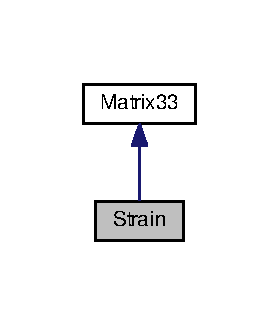
\includegraphics[width=134pt]{d6/d0f/classStrain__inherit__graph}
\end{center}
\end{figure}


\-Collaboration diagram for \-Strain\-:\nopagebreak
\begin{figure}[H]
\begin{center}
\leavevmode
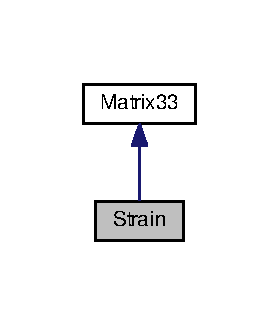
\includegraphics[width=134pt]{db/db8/classStrain__coll__graph}
\end{center}
\end{figure}
\subsection*{\-Public \-Member \-Functions}
\begin{DoxyCompactItemize}
\item 
\hyperlink{classStrain_ad7580e057dd173ba4a4609f4edfe6e38}{\-Strain} ()
\begin{DoxyCompactList}\small\item\em \-Default constructor. \end{DoxyCompactList}\item 
\hyperlink{classStrain_a808b5a0e273cc87e19138f3be221fe53}{\-Strain} (double $\ast$principal, double $\ast$shear)
\begin{DoxyCompactList}\small\item\em \-Constructor specifying the principal and shear strains. \end{DoxyCompactList}\item 
\hyperlink{classStrain_a411164cde64f3c51520440f928fb8fd8}{\-Strain} (\hyperlink{classMatrix33}{\-Matrix33} m)
\begin{DoxyCompactList}\small\item\em \-Constructor specifying the full matrix. \end{DoxyCompactList}\item 
void \hyperlink{classStrain_a53d0c01b18a8c70da97ad4aaeb924f14}{populate\-Matrix} ()
\begin{DoxyCompactList}\small\item\em \-Construct the strain tensor from the principal and shear strains. \end{DoxyCompactList}\item 
\hyperlink{classVector3d}{\-Vector3d} \hyperlink{classStrain_a441936c89c087ec4ca9927e914a2cece}{get\-Principal\-Strains} () const 
\begin{DoxyCompactList}\small\item\em \-Get the principal strains. \end{DoxyCompactList}\item 
\hyperlink{classVector3d}{\-Vector3d} \hyperlink{classStrain_a12320d54bd51c0e31159da2d30a8f380}{get\-Shear\-Strains} () const 
\begin{DoxyCompactList}\small\item\em \-Get the shear strains. \end{DoxyCompactList}\item 
\hyperlink{classStrain}{\-Strain} \hyperlink{classStrain_a39acbb854eea7868d2b88c6106e80d18}{rotate} (\hyperlink{classRotationMatrix}{\-Rotation\-Matrix} alpha)
\begin{DoxyCompactList}\small\item\em \-Rotate the strain tensor from one coordinate system to another. \end{DoxyCompactList}\item 
void \hyperlink{classMatrix33_a6cdcec77fd089b2e73ad7ae85ecff30b}{set\-Value} (int row, int column, double value)
\begin{DoxyCompactList}\small\item\em \-Function to set the value of an element indicated by its position. \end{DoxyCompactList}\item 
double \hyperlink{classMatrix33_ab53b3e37ad830a87a804cf26311ba088}{get\-Value} (int row, int column) const 
\begin{DoxyCompactList}\small\item\em \-Returns the value of the element located by the row and column indices provided. \end{DoxyCompactList}\item 
\hyperlink{classMatrix33}{\-Matrix33} \hyperlink{classMatrix33_a07b999a7b1c905f3c98ba3792e6fa33f}{adjugate} () const 
\begin{DoxyCompactList}\small\item\em \-Returns the adjugate matrix of the present matrix. \end{DoxyCompactList}\item 
\hyperlink{classMatrix33}{\-Matrix33} \hyperlink{classMatrix33_a64418c1a8836b38526fdfd7ffcc79cfd}{transpose} () const 
\begin{DoxyCompactList}\small\item\em \-Returns the transpose of the present matrix. \end{DoxyCompactList}\item 
\hyperlink{classMatrix33}{\-Matrix33} \hyperlink{classMatrix33_adc58ec5739c9250ff1150c725d0e868e}{operator+} (const \hyperlink{classMatrix33}{\-Matrix33} \&) const 
\begin{DoxyCompactList}\small\item\em \-Operator for addition of two matrices. \end{DoxyCompactList}\item 
void \hyperlink{classMatrix33_acb59e59d3937e075521f478ba83b7165}{operator+=} (const \hyperlink{classMatrix33}{\-Matrix33} \&)
\begin{DoxyCompactList}\small\item\em \-Operator for reflexive addition of two matrices. \end{DoxyCompactList}\item 
\hyperlink{classMatrix33}{\-Matrix33} \hyperlink{classMatrix33_a372f71ec208bb6d3045acd4324b7cb06}{operator-\/} (const \hyperlink{classMatrix33}{\-Matrix33} \&) const 
\begin{DoxyCompactList}\small\item\em \-Operator for the subtraction of two matrices. \end{DoxyCompactList}\item 
void \hyperlink{classMatrix33_abc889e10a9c7c532195c7031c1344a74}{operator-\/=} (const \hyperlink{classMatrix33}{\-Matrix33} \&)
\begin{DoxyCompactList}\small\item\em \-Operator for reflexive subtraction of two matrices. \end{DoxyCompactList}\item 
\hyperlink{classMatrix33}{\-Matrix33} \hyperlink{classMatrix33_a6992fd2bb0b6e9ad71b5d3481c4e3e1a}{operator$\ast$} (const double \&) const 
\begin{DoxyCompactList}\small\item\em \-Operator for scaling the matrix by a scalar. \end{DoxyCompactList}\item 
\hyperlink{classMatrix33}{\-Matrix33} \hyperlink{classMatrix33_a525f14614255ff81c0cbab8060e8e065}{operator$\ast$} (const \hyperlink{classMatrix33}{\-Matrix33} \&) const 
\begin{DoxyCompactList}\small\item\em \-Operator for the multiplication of two matrices. \end{DoxyCompactList}\item 
\hyperlink{classVector3d}{\-Vector3d} \hyperlink{classMatrix33_a601584a1edbaae7c6a2a2874605d6f61}{operator$\ast$} (const \hyperlink{classVector3d}{\-Vector3d} \&) const 
\begin{DoxyCompactList}\small\item\em \-Operator for the multiplication of a matrix with a vector. \end{DoxyCompactList}\item 
void \hyperlink{classMatrix33_a83162791813bef030b1ceb5df3c5cae3}{operator$\ast$=} (const double \&)
\begin{DoxyCompactList}\small\item\em \-Operator for reflexive scaling of the matrix by a scalar. \end{DoxyCompactList}\item 
void \hyperlink{classMatrix33_ac3937bdeb034cc83b4adcad16cd58a26}{operator$\ast$=} (const \hyperlink{classMatrix33}{\-Matrix33} \&)
\begin{DoxyCompactList}\small\item\em \-Operator for reflexive multiplication of two matrices. \end{DoxyCompactList}\item 
double \hyperlink{classMatrix33_a15b37caa6ab0d9f4a9f0d95846abd675}{operator$\sim$} () const 
\begin{DoxyCompactList}\small\item\em \-Determinant. \end{DoxyCompactList}\item 
\hyperlink{classMatrix33}{\-Matrix33} \hyperlink{classMatrix33_a1b822a20343a26b3c9bb7fd5c1247f37}{operator!} () const 
\begin{DoxyCompactList}\small\item\em \-Inverse. \end{DoxyCompactList}\end{DoxyCompactItemize}
\subsection*{\-Protected \-Attributes}
\begin{DoxyCompactItemize}
\item 
double \hyperlink{classStrain_a172c6ef4593e35bc9280a2dafde61475}{principal\-Strains} \mbox{[}3\mbox{]}
\item 
double \hyperlink{classStrain_afbc4d1b573860bda614a43f767b8b272}{shear\-Strains} \mbox{[}3\mbox{]}
\item 
double \hyperlink{classMatrix33_af7f01fa466616eb7c8eda2e4d9f85cdd}{x} \mbox{[}3\mbox{]}\mbox{[}3\mbox{]}
\begin{DoxyCompactList}\small\item\em \-Array containing the elements of the matrix. \end{DoxyCompactList}\end{DoxyCompactItemize}


\subsection{\-Detailed \-Description}
\hyperlink{classStrain}{\-Strain} class to represent the strain tensor. 

\-The member functions of this class construct the symmetric strain tensor and operate on it. 

\-Definition at line 21 of file strain.\-h.



\subsection{\-Constructor \& \-Destructor \-Documentation}
\hypertarget{classStrain_ad7580e057dd173ba4a4609f4edfe6e38}{\index{\-Strain@{\-Strain}!\-Strain@{\-Strain}}
\index{\-Strain@{\-Strain}!Strain@{\-Strain}}
\subsubsection[{\-Strain}]{\setlength{\rightskip}{0pt plus 5cm}{\bf \-Strain\-::\-Strain} (
\begin{DoxyParamCaption}
{}
\end{DoxyParamCaption}
)}}\label{d1/d3c/classStrain_ad7580e057dd173ba4a4609f4edfe6e38}


\-Default constructor. 

\-Initializes the strain tensor with zeros. 

\-Definition at line 16 of file strain.\-cpp.


\begin{DoxyCode}
{
  int i, j;

  for (i=0; i<3; i++)
    {
      principalStrains [i] = 0.0;
      shearStrains [i] = 0.0;
    }

  this->populateMatrix ();
}
\end{DoxyCode}
\hypertarget{classStrain_a808b5a0e273cc87e19138f3be221fe53}{\index{\-Strain@{\-Strain}!\-Strain@{\-Strain}}
\index{\-Strain@{\-Strain}!Strain@{\-Strain}}
\subsubsection[{\-Strain}]{\setlength{\rightskip}{0pt plus 5cm}{\bf \-Strain\-::\-Strain} (
\begin{DoxyParamCaption}
\item[{double $\ast$}]{principal, }
\item[{double $\ast$}]{shear}
\end{DoxyParamCaption}
)}}\label{d1/d3c/classStrain_a808b5a0e273cc87e19138f3be221fe53}


\-Constructor specifying the principal and shear strains. 

\-The principal and shear strains are provided in the arguments and the symmetrical strain tensor is contstructed using them. 
\begin{DoxyParams}{\-Parameters}
{\em principal} & \-Pointer to the array containing principal strains. \\
\hline
{\em shear} & \-Pointer to the array containing shear strains. \\
\hline
\end{DoxyParams}


\-Definition at line 35 of file strain.\-cpp.


\begin{DoxyCode}
{
  int i;

  for (i=0; i<3; i++)
    {
      this->principalStrains [i] = principal [i];
      this->shearStrains [i] = shear [i];
    }

  this->populateMatrix ();
}
\end{DoxyCode}
\hypertarget{classStrain_a411164cde64f3c51520440f928fb8fd8}{\index{\-Strain@{\-Strain}!\-Strain@{\-Strain}}
\index{\-Strain@{\-Strain}!Strain@{\-Strain}}
\subsubsection[{\-Strain}]{\setlength{\rightskip}{0pt plus 5cm}{\bf \-Strain\-::\-Strain} (
\begin{DoxyParamCaption}
\item[{{\bf \-Matrix33}}]{m}
\end{DoxyParamCaption}
)}}\label{d1/d3c/classStrain_a411164cde64f3c51520440f928fb8fd8}


\-Constructor specifying the full matrix. 

\-This constructor accepts the full strain matrix as input and extracts the principal and shear strain components. 
\begin{DoxyParams}{\-Parameters}
{\em m} & \hyperlink{classMatrix33}{\-Matrix33} variable containing the full strain tensor. \\
\hline
\end{DoxyParams}


\-Definition at line 53 of file strain.\-cpp.


\begin{DoxyCode}
{
  int i, j;
  bool symmetry = true;

  // Verify symmetry
  for (i=0; i<3; i++)
    {
      for (j=0; j<3; j++)
        {
          if (m.getValue(i,j) != m.getValue(j,i))
            {
              symmetry = false;
              break;
            }
        }
    }

  if (symmetry)
    {
      // The matrix is symmetrical
      this->principalStrains [0] = m.getValue(0,0);
      this->principalStrains [1] = m.getValue(1,1);
      this->principalStrains [2] = m.getValue(2,2);

      this->shearStrains [0] = m.getValue(0,1);
      this->shearStrains [1] = m.getValue(0,2);
      this->shearStrains [2] = m.getValue(1,2);
    }
  else
    {
      // The matrix is asymmetrical
      // A zero matrix will be returned
      for (i=0; i<3; i++)
        {
          this->principalStrains[i] = 0.0;
          this->shearStrains[i] = 0.0;
        }
    }

  this->populateMatrix ();
}
\end{DoxyCode}


\subsection{\-Member \-Function \-Documentation}
\hypertarget{classMatrix33_a07b999a7b1c905f3c98ba3792e6fa33f}{\index{\-Strain@{\-Strain}!adjugate@{adjugate}}
\index{adjugate@{adjugate}!Strain@{\-Strain}}
\subsubsection[{adjugate}]{\setlength{\rightskip}{0pt plus 5cm}{\bf \-Matrix33} {\bf \-Matrix33\-::adjugate} (
\begin{DoxyParamCaption}
{}
\end{DoxyParamCaption}
) const\hspace{0.3cm}{\ttfamily  \mbox{[}inherited\mbox{]}}}}\label{de/d82/classMatrix33_a07b999a7b1c905f3c98ba3792e6fa33f}


\-Returns the adjugate matrix of the present matrix. 

\-The adjugate matrix of the present matrix is returned. \-The adjugate matrix is calculated by evaluating the determinant of the cofactor matrix of each element, and then replacing the corresponding element position by the value of the determinant. \-This operation is useful in calculating the inverse of a matrix. \begin{DoxyReturn}{\-Returns}
\-The adjugate matrix of the present matrix. 
\end{DoxyReturn}


\-Definition at line 129 of file matrix33.\-cpp.


\begin{DoxyCode}
{
  Matrix33 adj;
  
  adj.setValue(0, 0, ((this->x[1][1]*this->x[2][2]) - (this->x[1][2]*this->x[2]
      [1])));
  adj.setValue(0, 1, ((this->x[1][2]*this->x[2][0]) - (this->x[1][0]*this->x[2]
      [2])));
  adj.setValue(0, 2, ((this->x[1][0]*this->x[2][1]) - (this->x[1][1]*this->x[2]
      [0])));
  
  adj.setValue(1, 0, ((this->x[2][1]*this->x[0][2]) - (this->x[0][1]*this->x[2]
      [2])));
  adj.setValue(1, 1, ((this->x[2][2]*this->x[0][0]) - (this->x[2][0]*this->x[0]
      [2])));
  adj.setValue(1, 2, ((this->x[2][0]*this->x[0][1]) - (this->x[2][1]*this->x[0]
      [0])));
  
  adj.setValue(2, 0, ((this->x[0][1]*this->x[1][2]) - (this->x[0][2]*this->x[1]
      [1])));
  adj.setValue(2, 1, ((this->x[0][2]*this->x[1][0]) - (this->x[0][0]*this->x[1]
      [2])));
  adj.setValue(2, 2, ((this->x[0][0]*this->x[1][1]) - (this->x[1][0]*this->x[0]
      [1])));

  return (adj);
}
\end{DoxyCode}
\hypertarget{classStrain_a441936c89c087ec4ca9927e914a2cece}{\index{\-Strain@{\-Strain}!get\-Principal\-Strains@{get\-Principal\-Strains}}
\index{get\-Principal\-Strains@{get\-Principal\-Strains}!Strain@{\-Strain}}
\subsubsection[{get\-Principal\-Strains}]{\setlength{\rightskip}{0pt plus 5cm}{\bf \-Vector3d} {\bf \-Strain\-::get\-Principal\-Strains} (
\begin{DoxyParamCaption}
{}
\end{DoxyParamCaption}
) const}}\label{d1/d3c/classStrain_a441936c89c087ec4ca9927e914a2cece}


\-Get the principal strains. 

\-Returns a vector of type \hyperlink{classVector3d}{\-Vector3d} with the principal strains\-: s11 s22 s33. \begin{DoxyReturn}{\-Returns}
\hyperlink{classVector3d}{\-Vector3d} variable with the principal strains. 
\end{DoxyReturn}


\-Definition at line 116 of file strain.\-cpp.


\begin{DoxyCode}
{
  return ( Vector3d (this->principalStrains [0],
                     this->principalStrains [1],
                     this->principalStrains [2] ) );
}
\end{DoxyCode}
\hypertarget{classStrain_a12320d54bd51c0e31159da2d30a8f380}{\index{\-Strain@{\-Strain}!get\-Shear\-Strains@{get\-Shear\-Strains}}
\index{get\-Shear\-Strains@{get\-Shear\-Strains}!Strain@{\-Strain}}
\subsubsection[{get\-Shear\-Strains}]{\setlength{\rightskip}{0pt plus 5cm}{\bf \-Vector3d} {\bf \-Strain\-::get\-Shear\-Strains} (
\begin{DoxyParamCaption}
{}
\end{DoxyParamCaption}
) const}}\label{d1/d3c/classStrain_a12320d54bd51c0e31159da2d30a8f380}


\-Get the shear strains. 

\-Returns a vector of type \hyperlink{classVector3d}{\-Vector3d} with the shear strains\-: s12 s13 s23. \begin{DoxyReturn}{\-Returns}
\hyperlink{classVector3d}{\-Vector3d} variable with the shear strains. 
\end{DoxyReturn}


\-Definition at line 128 of file strain.\-cpp.


\begin{DoxyCode}
{
  return ( Vector3d (this->shearStrains [0],
                     this->shearStrains [1],
                     this->shearStrains [2] ) );
}
\end{DoxyCode}
\hypertarget{classMatrix33_ab53b3e37ad830a87a804cf26311ba088}{\index{\-Strain@{\-Strain}!get\-Value@{get\-Value}}
\index{get\-Value@{get\-Value}!Strain@{\-Strain}}
\subsubsection[{get\-Value}]{\setlength{\rightskip}{0pt plus 5cm}double {\bf \-Matrix33\-::get\-Value} (
\begin{DoxyParamCaption}
\item[{int}]{row, }
\item[{int}]{column}
\end{DoxyParamCaption}
) const\hspace{0.3cm}{\ttfamily  \mbox{[}inherited\mbox{]}}}}\label{de/d82/classMatrix33_ab53b3e37ad830a87a804cf26311ba088}


\-Returns the value of the element located by the row and column indices provided. 

\-The value of the element indicated by the arguments row and column is returned. \-The values of row and column must correspond to array indices, and thus can be one of 0, 1 and 2. \-In any other case 0.\-0 is returned. 
\begin{DoxyParams}{\-Parameters}
{\em row} & \-Row index of the element. \\
\hline
{\em column} & \-Column index of the element. \\
\hline
\end{DoxyParams}
\begin{DoxyReturn}{\-Returns}
\-Value of the element located at the given position. 
\end{DoxyReturn}


\-Definition at line 111 of file matrix33.\-cpp.


\begin{DoxyCode}
{
  if (row>=0 && row<3)
    {
      if (column>=0 && column<3)
        {
          return (this->x[row][column]);
        }
    }
  
  return (0.0);
}
\end{DoxyCode}
\hypertarget{classMatrix33_a1b822a20343a26b3c9bb7fd5c1247f37}{\index{\-Strain@{\-Strain}!operator!@{operator!}}
\index{operator!@{operator!}!Strain@{\-Strain}}
\subsubsection[{operator!}]{\setlength{\rightskip}{0pt plus 5cm}{\bf \-Matrix33} {\bf \-Matrix33\-::operator!} (
\begin{DoxyParamCaption}
{}
\end{DoxyParamCaption}
) const\hspace{0.3cm}{\ttfamily  \mbox{[}inherited\mbox{]}}}}\label{de/d82/classMatrix33_a1b822a20343a26b3c9bb7fd5c1247f37}


\-Inverse. 

\-Returns in a new matrix the inverse of the current matrix. \-If the current matrix is non-\/invertible, a zero matrix is returned. \begin{DoxyReturn}{\-Returns}
\-Matrix with the inverse of the current matrix. \-If the current matrix is non-\/invertible, a zero matrix is returned. 
\end{DoxyReturn}


\-Definition at line 374 of file matrix33.\-cpp.


\begin{DoxyCode}
{
  Matrix33 r;   // Result matrix
  
  double determinant = ~(*this);
  
  if (determinant == 0.0)
    {
      // The matrix is non-invertible
      return (r);       // Zero matrix
    }
  
  // If we are still here, the matrix is invertible
  
  //  Transpose
  Matrix33 tr = this->transpose();
  
  // Find Adjugate matrix
  Matrix33 adj = tr.adjugate();
  
  // Calculate the inverse by dividing the adjugate matrix by the determinant
  r = adj * (1.0/determinant);
  
  return (r);
}
\end{DoxyCode}
\hypertarget{classMatrix33_a6992fd2bb0b6e9ad71b5d3481c4e3e1a}{\index{\-Strain@{\-Strain}!operator$\ast$@{operator$\ast$}}
\index{operator$\ast$@{operator$\ast$}!Strain@{\-Strain}}
\subsubsection[{operator$\ast$}]{\setlength{\rightskip}{0pt plus 5cm}{\bf \-Matrix33} \-Matrix33\-::operator$\ast$ (
\begin{DoxyParamCaption}
\item[{const double \&}]{p}
\end{DoxyParamCaption}
) const\hspace{0.3cm}{\ttfamily  \mbox{[}inherited\mbox{]}}}}\label{de/d82/classMatrix33_a6992fd2bb0b6e9ad71b5d3481c4e3e1a}


\-Operator for scaling the matrix by a scalar. 

\-Scales the current matrix by the scalar provided and returns the result in a third matrix. \begin{DoxyReturn}{\-Returns}
\-Matrix containing the result of scaling the current matrix by the scalar provided as argument. 
\end{DoxyReturn}


\-Definition at line 253 of file matrix33.\-cpp.


\begin{DoxyCode}
{
  int i, j;
  Matrix33 r;
  
  for (i=0; i<3; i++)
    {
      for (j=0; j<3; j++)
        {
          r.setValue(i, j, (this->x[i][j] * p));
        }
    }
  
  return (r);
}
\end{DoxyCode}
\hypertarget{classMatrix33_a525f14614255ff81c0cbab8060e8e065}{\index{\-Strain@{\-Strain}!operator$\ast$@{operator$\ast$}}
\index{operator$\ast$@{operator$\ast$}!Strain@{\-Strain}}
\subsubsection[{operator$\ast$}]{\setlength{\rightskip}{0pt plus 5cm}{\bf \-Matrix33} \-Matrix33\-::operator$\ast$ (
\begin{DoxyParamCaption}
\item[{const {\bf \-Matrix33} \&}]{p}
\end{DoxyParamCaption}
) const\hspace{0.3cm}{\ttfamily  \mbox{[}inherited\mbox{]}}}}\label{de/d82/classMatrix33_a525f14614255ff81c0cbab8060e8e065}


\-Operator for the multiplication of two matrices. 

\-Multiplies the current matrix with another 3x3 matrix and returns the result in a new matrix. \begin{DoxyReturn}{\-Returns}
\-The result of the multiplication of the current matrix with the one provided as argument. 
\end{DoxyReturn}


\-Definition at line 291 of file matrix33.\-cpp.


\begin{DoxyCode}
{
  int i, j, k;
  Matrix33 r;
  double s;
  
  for (i=0; i<3; i++)
    {
      for (j=0; j<3; j++)
        {
          s = 0.0;
          for (k=0; k<3; k++)
            {
              s += this->x[i][k] * p.getValue(k,j);
            }
          r.setValue (i, j, s);
        }
    }
  
  return (r);
}
\end{DoxyCode}
\hypertarget{classMatrix33_a601584a1edbaae7c6a2a2874605d6f61}{\index{\-Strain@{\-Strain}!operator$\ast$@{operator$\ast$}}
\index{operator$\ast$@{operator$\ast$}!Strain@{\-Strain}}
\subsubsection[{operator$\ast$}]{\setlength{\rightskip}{0pt plus 5cm}{\bf \-Vector3d} \-Matrix33\-::operator$\ast$ (
\begin{DoxyParamCaption}
\item[{const {\bf \-Vector3d} \&}]{v}
\end{DoxyParamCaption}
) const\hspace{0.3cm}{\ttfamily  \mbox{[}inherited\mbox{]}}}}\label{de/d82/classMatrix33_a601584a1edbaae7c6a2a2874605d6f61}


\-Operator for the multiplication of a matrix with a vector. 

\-Returns in a vector the result of the multiplication of the current matrix with the provided vector. \begin{DoxyReturn}{\-Returns}
\-The vector resulting from the multiplication of the current matrix with a vector. 
\end{DoxyReturn}


\-Definition at line 333 of file matrix33.\-cpp.


\begin{DoxyCode}
{
  Vector3d r(0.0, 0.0, 0.0);
  double s;
  int i, j;
  
  for (i=0; i<3; i++)
    {
      s = 0.0;
      for (j=0; j<3; j++)
        {
          s += this->x[i][j] * v.getValue(j);
        }
      r.setValue (i, s);
    }
  
  return (r);
}
\end{DoxyCode}
\hypertarget{classMatrix33_a83162791813bef030b1ceb5df3c5cae3}{\index{\-Strain@{\-Strain}!operator$\ast$=@{operator$\ast$=}}
\index{operator$\ast$=@{operator$\ast$=}!Strain@{\-Strain}}
\subsubsection[{operator$\ast$=}]{\setlength{\rightskip}{0pt plus 5cm}void \-Matrix33\-::operator$\ast$= (
\begin{DoxyParamCaption}
\item[{const double \&}]{p}
\end{DoxyParamCaption}
)\hspace{0.3cm}{\ttfamily  \mbox{[}inherited\mbox{]}}}}\label{de/d82/classMatrix33_a83162791813bef030b1ceb5df3c5cae3}


\-Operator for reflexive scaling of the matrix by a scalar. 

\-Scales the current matrix by the scalar provided and populates the current matrix elements with the result. 

\-Definition at line 273 of file matrix33.\-cpp.


\begin{DoxyCode}
{
  int i, j;
  
  for (i=0; i<3; i++)
    {
      for (j=0; j<3; j++)
        {
          this->x[i][j] *= p;
        }
    }
}
\end{DoxyCode}
\hypertarget{classMatrix33_ac3937bdeb034cc83b4adcad16cd58a26}{\index{\-Strain@{\-Strain}!operator$\ast$=@{operator$\ast$=}}
\index{operator$\ast$=@{operator$\ast$=}!Strain@{\-Strain}}
\subsubsection[{operator$\ast$=}]{\setlength{\rightskip}{0pt plus 5cm}void \-Matrix33\-::operator$\ast$= (
\begin{DoxyParamCaption}
\item[{const {\bf \-Matrix33} \&}]{p}
\end{DoxyParamCaption}
)\hspace{0.3cm}{\ttfamily  \mbox{[}inherited\mbox{]}}}}\label{de/d82/classMatrix33_ac3937bdeb034cc83b4adcad16cd58a26}


\-Operator for reflexive multiplication of two matrices. 

\-Multiplies the current matrix with another 3x3 matrix and populates the elements of the current matrix with the result. 

\-Definition at line 317 of file matrix33.\-cpp.


\begin{DoxyCode}
{
  Matrix33* r = new Matrix33;
  
  *r = (*this) * p;
  *this = *r;
  
  delete(r);
  r = NULL;
}
\end{DoxyCode}
\hypertarget{classMatrix33_adc58ec5739c9250ff1150c725d0e868e}{\index{\-Strain@{\-Strain}!operator+@{operator+}}
\index{operator+@{operator+}!Strain@{\-Strain}}
\subsubsection[{operator+}]{\setlength{\rightskip}{0pt plus 5cm}{\bf \-Matrix33} \-Matrix33\-::operator+ (
\begin{DoxyParamCaption}
\item[{const {\bf \-Matrix33} \&}]{p}
\end{DoxyParamCaption}
) const\hspace{0.3cm}{\ttfamily  \mbox{[}inherited\mbox{]}}}}\label{de/d82/classMatrix33_adc58ec5739c9250ff1150c725d0e868e}


\-Operator for addition of two matrices. 

\-Adds the current matrix to the provided matrix and returns a third matrix with the result. \begin{DoxyReturn}{\-Returns}
\-Matrix containing the sum of the present matrix and the one provided. 
\end{DoxyReturn}


\-Definition at line 175 of file matrix33.\-cpp.


\begin{DoxyCode}
{
  int i, j;
  Matrix33 r;
  
  for (i=0; i<3; i++)
    {
      for (j=0; j<3; j++)
        {
          r.setValue(i, j, (this->x[i][j] + p.getValue(i, j)));
        }
    }
  
  return (r);
}
\end{DoxyCode}
\hypertarget{classMatrix33_acb59e59d3937e075521f478ba83b7165}{\index{\-Strain@{\-Strain}!operator+=@{operator+=}}
\index{operator+=@{operator+=}!Strain@{\-Strain}}
\subsubsection[{operator+=}]{\setlength{\rightskip}{0pt plus 5cm}void \-Matrix33\-::operator+= (
\begin{DoxyParamCaption}
\item[{const {\bf \-Matrix33} \&}]{p}
\end{DoxyParamCaption}
)\hspace{0.3cm}{\ttfamily  \mbox{[}inherited\mbox{]}}}}\label{de/d82/classMatrix33_acb59e59d3937e075521f478ba83b7165}


\-Operator for reflexive addition of two matrices. 

\-Adds the current matrix to the provided matrix and populates the current matrix elements with the result. 

\-Definition at line 195 of file matrix33.\-cpp.


\begin{DoxyCode}
{
  int i, j;
  
  for (i=0; i<3; i++)
    {
      for (j=0; j<3; j++)
        {
          this->x[i][j] += p.getValue(i, j);
        }
    }
}
\end{DoxyCode}
\hypertarget{classMatrix33_a372f71ec208bb6d3045acd4324b7cb06}{\index{\-Strain@{\-Strain}!operator-\/@{operator-\/}}
\index{operator-\/@{operator-\/}!Strain@{\-Strain}}
\subsubsection[{operator-\/}]{\setlength{\rightskip}{0pt plus 5cm}{\bf \-Matrix33} \-Matrix33\-::operator-\/ (
\begin{DoxyParamCaption}
\item[{const {\bf \-Matrix33} \&}]{p}
\end{DoxyParamCaption}
) const\hspace{0.3cm}{\ttfamily  \mbox{[}inherited\mbox{]}}}}\label{de/d82/classMatrix33_a372f71ec208bb6d3045acd4324b7cb06}


\-Operator for the subtraction of two matrices. 

\-Subtracts the given matrix from the current matrix and returns the result in a new matrix. \begin{DoxyReturn}{\-Returns}
\-Matrix containing the result of subtracting the provided matrix from the current matrix. 
\end{DoxyReturn}


\-Definition at line 214 of file matrix33.\-cpp.


\begin{DoxyCode}
{
  int i, j;
  Matrix33 r;
  
  for (i=0; i<3; i++)
    {
      for (j=0; j<3; j++)
        {
          r.setValue(i, j, (this->x[i][j] - p.getValue(i, j)));
        }
    }
  
  return (r);
}
\end{DoxyCode}
\hypertarget{classMatrix33_abc889e10a9c7c532195c7031c1344a74}{\index{\-Strain@{\-Strain}!operator-\/=@{operator-\/=}}
\index{operator-\/=@{operator-\/=}!Strain@{\-Strain}}
\subsubsection[{operator-\/=}]{\setlength{\rightskip}{0pt plus 5cm}void \-Matrix33\-::operator-\/= (
\begin{DoxyParamCaption}
\item[{const {\bf \-Matrix33} \&}]{p}
\end{DoxyParamCaption}
)\hspace{0.3cm}{\ttfamily  \mbox{[}inherited\mbox{]}}}}\label{de/d82/classMatrix33_abc889e10a9c7c532195c7031c1344a74}


\-Operator for reflexive subtraction of two matrices. 

\-Subtracts the given matrix from the current matrix and populates the current matrix with the result. 

\-Definition at line 234 of file matrix33.\-cpp.


\begin{DoxyCode}
{
  int i, j;
  
  for (i=0; i<3; i++)
    {
      for (j=0; j<3; j++)
        {
          this->x[i][j] -= p.getValue(i, j);
        }
    }
}
\end{DoxyCode}
\hypertarget{classMatrix33_a15b37caa6ab0d9f4a9f0d95846abd675}{\index{\-Strain@{\-Strain}!operator$\sim$@{operator$\sim$}}
\index{operator$\sim$@{operator$\sim$}!Strain@{\-Strain}}
\subsubsection[{operator$\sim$}]{\setlength{\rightskip}{0pt plus 5cm}double {\bf \-Matrix33\-::operator$\sim$} (
\begin{DoxyParamCaption}
{}
\end{DoxyParamCaption}
) const\hspace{0.3cm}{\ttfamily  \mbox{[}inherited\mbox{]}}}}\label{de/d82/classMatrix33_a15b37caa6ab0d9f4a9f0d95846abd675}


\-Determinant. 

\-Calculates the determinant of the current matrix. \begin{DoxyReturn}{\-Returns}
\-Returns the determinant of the current matrix. 
\end{DoxyReturn}


\-Definition at line 358 of file matrix33.\-cpp.


\begin{DoxyCode}
{
  double d = 0.0;
  
  d += this->x[0][0] * ( (this->x[1][1]*this->x[2][2]) - (this->x[2][1]*this->x
      [1][2]) );
  d += this->x[0][1] * ( (this->x[1][2]*this->x[2][0]) - (this->x[1][0]*this->x
      [2][2]) );
  d += this->x[0][2] * ( (this->x[1][0]*this->x[2][1]) - (this->x[2][0]*this->x
      [1][1]) );
  
  return (d);
}
\end{DoxyCode}
\hypertarget{classStrain_a53d0c01b18a8c70da97ad4aaeb924f14}{\index{\-Strain@{\-Strain}!populate\-Matrix@{populate\-Matrix}}
\index{populate\-Matrix@{populate\-Matrix}!Strain@{\-Strain}}
\subsubsection[{populate\-Matrix}]{\setlength{\rightskip}{0pt plus 5cm}void {\bf \-Strain\-::populate\-Matrix} (
\begin{DoxyParamCaption}
{}
\end{DoxyParamCaption}
)}}\label{d1/d3c/classStrain_a53d0c01b18a8c70da97ad4aaeb924f14}


\-Construct the strain tensor from the principal and shear strains. 

\-Takes the values in principal\-Strains and shear\-Strains and constructs the symmetrical strain matrix. 

\-Definition at line 100 of file strain.\-cpp.


\begin{DoxyCode}
{
  this->x[0][0] = this->principalStrains [0];
  this->x[1][1] = this->principalStrains [1];
  this->x[2][2] = this->principalStrains [2];

  this->x[0][1] = this->x[1][0] = this->shearStrains [0];
  this->x[0][2] = this->x[2][0] = this->shearStrains [1];
  this->x[1][2] = this->x[2][1] = this->shearStrains [2];
}
\end{DoxyCode}
\hypertarget{classStrain_a39acbb854eea7868d2b88c6106e80d18}{\index{\-Strain@{\-Strain}!rotate@{rotate}}
\index{rotate@{rotate}!Strain@{\-Strain}}
\subsubsection[{rotate}]{\setlength{\rightskip}{0pt plus 5cm}{\bf \-Strain} {\bf \-Strain\-::rotate} (
\begin{DoxyParamCaption}
\item[{{\bf \-Rotation\-Matrix}}]{alpha}
\end{DoxyParamCaption}
)}}\label{d1/d3c/classStrain_a39acbb854eea7868d2b88c6106e80d18}


\-Rotate the strain tensor from one coordinate system to another. 

\-Rotates the present strain matrix from one coordinate system to another using the rotation matrix supplied. \-The result is returned in a new \hyperlink{classStrain}{\-Strain} matrix. 
\begin{DoxyParams}{\-Parameters}
{\em alpha} & \-Rotation matrix. \\
\hline
\end{DoxyParams}
\begin{DoxyReturn}{\-Returns}
\-Rotated strain tensor. 
\end{DoxyReturn}


\-Definition at line 141 of file strain.\-cpp.


\begin{DoxyCode}
{
  // Transpose
  RotationMatrix alphaT (alpha.transpose());

  // Rotate the strain matrix
  Strain sNew = Strain (alpha * (*this) * alphaT);

  return (sNew);
}
\end{DoxyCode}
\hypertarget{classMatrix33_a6cdcec77fd089b2e73ad7ae85ecff30b}{\index{\-Strain@{\-Strain}!set\-Value@{set\-Value}}
\index{set\-Value@{set\-Value}!Strain@{\-Strain}}
\subsubsection[{set\-Value}]{\setlength{\rightskip}{0pt plus 5cm}void {\bf \-Matrix33\-::set\-Value} (
\begin{DoxyParamCaption}
\item[{int}]{row, }
\item[{int}]{column, }
\item[{double}]{value}
\end{DoxyParamCaption}
)\hspace{0.3cm}{\ttfamily  \mbox{[}inherited\mbox{]}}}}\label{de/d82/classMatrix33_a6cdcec77fd089b2e73ad7ae85ecff30b}


\-Function to set the value of an element indicated by its position. 

\-The element indicated by the arguments row and column is set to the value provided. \-The values of row and column must correspond to array indices, and thus can be one of 0, 1 and 2. \-In any other case 0.\-0 is returned. 
\begin{DoxyParams}{\-Parameters}
{\em row} & \-Row index of the element. \\
\hline
{\em column} & \-Column index of the element. \\
\hline
{\em value} & \-Value that the element is to be set to. \\
\hline
\end{DoxyParams}


\-Definition at line 93 of file matrix33.\-cpp.


\begin{DoxyCode}
{
  if (row>=0 && row<3)
    {
      if (column>=0 && column<3)
        {
          this->x[row][column] = value;
        }
    }
}
\end{DoxyCode}
\hypertarget{classMatrix33_a64418c1a8836b38526fdfd7ffcc79cfd}{\index{\-Strain@{\-Strain}!transpose@{transpose}}
\index{transpose@{transpose}!Strain@{\-Strain}}
\subsubsection[{transpose}]{\setlength{\rightskip}{0pt plus 5cm}{\bf \-Matrix33} {\bf \-Matrix33\-::transpose} (
\begin{DoxyParamCaption}
{}
\end{DoxyParamCaption}
) const\hspace{0.3cm}{\ttfamily  \mbox{[}inherited\mbox{]}}}}\label{de/d82/classMatrix33_a64418c1a8836b38526fdfd7ffcc79cfd}


\-Returns the transpose of the present matrix. 

\-The transpose of a matrix is another matrix having rows identical to the columns of the present matrix, and vice-\/versa. \begin{DoxyReturn}{\-Returns}
\-The transpose of the present matrix. 
\end{DoxyReturn}


\-Definition at line 153 of file matrix33.\-cpp.


\begin{DoxyCode}
{
  Matrix33 tr;
  int i, j;

  for (i=0; i<3; i++)
    {
      for (j=0; j<3; j++)
        {
          tr.setValue (i, j, this->x[j][i]);
        }
    }
  return (tr);
}
\end{DoxyCode}


\subsection{\-Field \-Documentation}
\hypertarget{classStrain_a172c6ef4593e35bc9280a2dafde61475}{\index{\-Strain@{\-Strain}!principal\-Strains@{principal\-Strains}}
\index{principal\-Strains@{principal\-Strains}!Strain@{\-Strain}}
\subsubsection[{principal\-Strains}]{\setlength{\rightskip}{0pt plus 5cm}double {\bf \-Strain\-::principal\-Strains}\mbox{[}3\mbox{]}\hspace{0.3cm}{\ttfamily  \mbox{[}protected\mbox{]}}}}\label{d1/d3c/classStrain_a172c6ef4593e35bc9280a2dafde61475}
\-The three principal strains\-: s11, s22, s33. 

\-Definition at line 27 of file strain.\-h.

\hypertarget{classStrain_afbc4d1b573860bda614a43f767b8b272}{\index{\-Strain@{\-Strain}!shear\-Strains@{shear\-Strains}}
\index{shear\-Strains@{shear\-Strains}!Strain@{\-Strain}}
\subsubsection[{shear\-Strains}]{\setlength{\rightskip}{0pt plus 5cm}double {\bf \-Strain\-::shear\-Strains}\mbox{[}3\mbox{]}\hspace{0.3cm}{\ttfamily  \mbox{[}protected\mbox{]}}}}\label{d1/d3c/classStrain_afbc4d1b573860bda614a43f767b8b272}
\-The three shear strains\-: s12, s13, s23, 

\-Definition at line 31 of file strain.\-h.

\hypertarget{classMatrix33_af7f01fa466616eb7c8eda2e4d9f85cdd}{\index{\-Strain@{\-Strain}!x@{x}}
\index{x@{x}!Strain@{\-Strain}}
\subsubsection[{x}]{\setlength{\rightskip}{0pt plus 5cm}double {\bf \-Matrix33\-::x}\mbox{[}3\mbox{]}\mbox{[}3\mbox{]}\hspace{0.3cm}{\ttfamily  \mbox{[}protected, inherited\mbox{]}}}}\label{de/d82/classMatrix33_af7f01fa466616eb7c8eda2e4d9f85cdd}


\-Array containing the elements of the matrix. 



\-Definition at line 26 of file matrix33.\-h.



\-The documentation for this class was generated from the following files\-:\begin{DoxyCompactItemize}
\item 
\hyperlink{strain_8h}{strain.\-h}\item 
\hyperlink{strain_8cpp}{strain.\-cpp}\end{DoxyCompactItemize}

\hypertarget{classStress}{\section{\-Stress \-Class \-Reference}
\label{d1/d1c/classStress}\index{\-Stress@{\-Stress}}
}


\hyperlink{classStress}{\-Stress} class to represent the stress tensor.  




{\ttfamily \#include $<$stress.\-h$>$}



\-Inheritance diagram for \-Stress\-:
\nopagebreak
\begin{figure}[H]
\begin{center}
\leavevmode
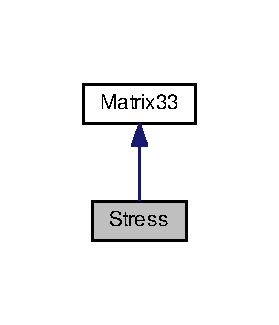
\includegraphics[width=134pt]{dd/d46/classStress__inherit__graph}
\end{center}
\end{figure}


\-Collaboration diagram for \-Stress\-:
\nopagebreak
\begin{figure}[H]
\begin{center}
\leavevmode
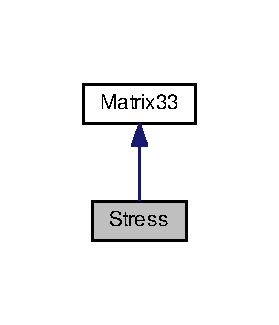
\includegraphics[width=134pt]{d7/dfa/classStress__coll__graph}
\end{center}
\end{figure}
\subsection*{\-Public \-Member \-Functions}
\begin{DoxyCompactItemize}
\item 
\hyperlink{classStress_aa01e83a3f6791cbadc5a368e3a40515e}{\-Stress} ()
\begin{DoxyCompactList}\small\item\em \-Default constructor. \end{DoxyCompactList}\item 
\hyperlink{classStress_ae4e2f6250e3bdd4d3d78a9c6bdde7bab}{\-Stress} (double $\ast$principal, double $\ast$shear)
\begin{DoxyCompactList}\small\item\em \-Constructor specifying the principal and shear stresses. \end{DoxyCompactList}\item 
void \hyperlink{classStress_aa395d5763df8feb4689e0c5524c9e562}{populate\-Matrix} ()
\begin{DoxyCompactList}\small\item\em \-Construct the stress tensor from the principal and shear stresses. \end{DoxyCompactList}\item 
double $\ast$ \hyperlink{classStress_aca57d2719f43701dd2ebf2ab00afa539}{get\-Principal\-Stresses} ()
\begin{DoxyCompactList}\small\item\em \-Get the principal stresses. \end{DoxyCompactList}\item 
double $\ast$ \hyperlink{classStress_afe8214b8e9061930e6598e1970fd61f5}{get\-Shear\-Stresses} ()
\begin{DoxyCompactList}\small\item\em \-Get the shear stresses. \end{DoxyCompactList}\item 
\hyperlink{classStress}{\-Stress} \hyperlink{classStress_a61fa75450c0232bb0fa427072d1b6a35}{rotate} (\hyperlink{classMatrix33}{\-Matrix33} alpha)
\begin{DoxyCompactList}\small\item\em \-Rotate the stress tensor from one coordinate system to another. \end{DoxyCompactList}\item 
void \hyperlink{classMatrix33_a6cdcec77fd089b2e73ad7ae85ecff30b}{set\-Value} (int row, int column, double value)
\begin{DoxyCompactList}\small\item\em \-Function to set the value of an element indicated by its position. \end{DoxyCompactList}\item 
double \hyperlink{classMatrix33_a849bbdf7b456ddacf7185b087fca4015}{get\-Value} (int row, int column)
\begin{DoxyCompactList}\small\item\em \-Returns the value of the element located by the row and column indices provided. \end{DoxyCompactList}\item 
\hyperlink{classMatrix33}{\-Matrix33} \hyperlink{classMatrix33_a4e64ab5af4921c24b8270a0c9050f4ba}{adjugate} ()
\begin{DoxyCompactList}\small\item\em \-Returns the adjugate matrix of the present matrix. \end{DoxyCompactList}\item 
\hyperlink{classMatrix33}{\-Matrix33} \hyperlink{classMatrix33_adc58ec5739c9250ff1150c725d0e868e}{operator+} (const \hyperlink{classMatrix33}{\-Matrix33} \&) const 
\begin{DoxyCompactList}\small\item\em \-Operator for addition of two matrices. \end{DoxyCompactList}\item 
void \hyperlink{classMatrix33_acb59e59d3937e075521f478ba83b7165}{operator+=} (const \hyperlink{classMatrix33}{\-Matrix33} \&)
\begin{DoxyCompactList}\small\item\em \-Operator for reflexive addition of two matrices. \end{DoxyCompactList}\item 
\hyperlink{classMatrix33}{\-Matrix33} \hyperlink{classMatrix33_a372f71ec208bb6d3045acd4324b7cb06}{operator-\/} (const \hyperlink{classMatrix33}{\-Matrix33} \&) const 
\begin{DoxyCompactList}\small\item\em \-Operator for the subtraction of two matrices. \end{DoxyCompactList}\item 
void \hyperlink{classMatrix33_abc889e10a9c7c532195c7031c1344a74}{operator-\/=} (const \hyperlink{classMatrix33}{\-Matrix33} \&)
\begin{DoxyCompactList}\small\item\em \-Operator for reflexive subtraction of two matrices. \end{DoxyCompactList}\item 
\hyperlink{classMatrix33}{\-Matrix33} \hyperlink{classMatrix33_a6992fd2bb0b6e9ad71b5d3481c4e3e1a}{operator$\ast$} (const double \&) const 
\begin{DoxyCompactList}\small\item\em \-Operator for scaling the matrix by a scalar. \end{DoxyCompactList}\item 
\hyperlink{classMatrix33}{\-Matrix33} \hyperlink{classMatrix33_a525f14614255ff81c0cbab8060e8e065}{operator$\ast$} (const \hyperlink{classMatrix33}{\-Matrix33} \&) const 
\begin{DoxyCompactList}\small\item\em \-Operator for the multiplication of two matrices. \end{DoxyCompactList}\item 
\hyperlink{classVector3d}{\-Vector3d} \hyperlink{classMatrix33_a601584a1edbaae7c6a2a2874605d6f61}{operator$\ast$} (const \hyperlink{classVector3d}{\-Vector3d} \&) const 
\begin{DoxyCompactList}\small\item\em \-Operator for the multiplication of a matrix with a vector. \end{DoxyCompactList}\item 
void \hyperlink{classMatrix33_a83162791813bef030b1ceb5df3c5cae3}{operator$\ast$=} (const double \&)
\begin{DoxyCompactList}\small\item\em \-Operator for reflexive scaling of the matrix by a scalar. \end{DoxyCompactList}\item 
void \hyperlink{classMatrix33_ac3937bdeb034cc83b4adcad16cd58a26}{operator$\ast$=} (const \hyperlink{classMatrix33}{\-Matrix33} \&)
\begin{DoxyCompactList}\small\item\em \-Operator for reflexive multiplication of two matrices. \end{DoxyCompactList}\item 
\hyperlink{classMatrix33}{\-Matrix33} \hyperlink{classMatrix33_ad4ab7b9674a44a297502282e1993ef54}{operator$^\wedge$} () const 
\begin{DoxyCompactList}\small\item\em \-Transpose. \end{DoxyCompactList}\item 
double \hyperlink{classMatrix33_a15b37caa6ab0d9f4a9f0d95846abd675}{operator$\sim$} () const 
\begin{DoxyCompactList}\small\item\em \-Determinant. \end{DoxyCompactList}\item 
\hyperlink{classMatrix33}{\-Matrix33} \hyperlink{classMatrix33_a1b822a20343a26b3c9bb7fd5c1247f37}{operator!} () const 
\begin{DoxyCompactList}\small\item\em \-Inverse. \end{DoxyCompactList}\end{DoxyCompactItemize}
\subsection*{\-Protected \-Attributes}
\begin{DoxyCompactItemize}
\item 
double \hyperlink{classStress_aea8c3e40aa59a89d7ba79d2c916050a6}{principal\-Stresses} \mbox{[}3\mbox{]}
\item 
double \hyperlink{classStress_a77e8705e56c2fb56826a638edf3f78bf}{shear\-Stresses} \mbox{[}3\mbox{]}
\item 
double \hyperlink{classMatrix33_af7f01fa466616eb7c8eda2e4d9f85cdd}{x} \mbox{[}3\mbox{]}\mbox{[}3\mbox{]}
\begin{DoxyCompactList}\small\item\em \-Array containing the elements of the matrix. \end{DoxyCompactList}\end{DoxyCompactItemize}


\subsection{\-Detailed \-Description}
\hyperlink{classStress}{\-Stress} class to represent the stress tensor. 

\-The member functions of this class construct the symmetric stress tensor and operate on it. 

\-Definition at line 20 of file stress.\-h.



\subsection{\-Constructor \& \-Destructor \-Documentation}
\hypertarget{classStress_aa01e83a3f6791cbadc5a368e3a40515e}{\index{\-Stress@{\-Stress}!\-Stress@{\-Stress}}
\index{\-Stress@{\-Stress}!Stress@{\-Stress}}
\subsubsection[{\-Stress}]{\setlength{\rightskip}{0pt plus 5cm}{\bf \-Stress\-::\-Stress} (
\begin{DoxyParamCaption}
{}
\end{DoxyParamCaption}
)}}\label{d1/d1c/classStress_aa01e83a3f6791cbadc5a368e3a40515e}


\-Default constructor. 

\-Initializes the stress tensor with zeros. 

\-Definition at line 16 of file stress.\-cpp.


\begin{DoxyCode}
{
  int i, j;
  
  for (i=0; i<3; i++)
    {
      principalStresses [i] = 0.0;
      shearStresses [i] = 0.0;
    }

  this->populateMatrix ();
}
\end{DoxyCode}
\hypertarget{classStress_ae4e2f6250e3bdd4d3d78a9c6bdde7bab}{\index{\-Stress@{\-Stress}!\-Stress@{\-Stress}}
\index{\-Stress@{\-Stress}!Stress@{\-Stress}}
\subsubsection[{\-Stress}]{\setlength{\rightskip}{0pt plus 5cm}{\bf \-Stress\-::\-Stress} (
\begin{DoxyParamCaption}
\item[{double $\ast$}]{principal, }
\item[{double $\ast$}]{shear}
\end{DoxyParamCaption}
)}}\label{d1/d1c/classStress_ae4e2f6250e3bdd4d3d78a9c6bdde7bab}


\-Constructor specifying the principal and shear stresses. 

\-The principal and shear stresses are provided in the arguments and the symmetrical stress tensor is contstructed using them. 
\begin{DoxyParams}{\-Parameters}
{\em principal} & \-Pointer to the array containing principal stresses. \\
\hline
{\em shear} & \-Pointer to the array containing shear stresses. \\
\hline
\end{DoxyParams}


\-Definition at line 35 of file stress.\-cpp.


\begin{DoxyCode}
{
  int i;
  
  for (i=0; i<3; i++)
    {
      this->principalStresses [i] = principal [i];
      this->shearStresses [i] = shear [i];
    }
  
  this->populateMatrix ();
}
\end{DoxyCode}


\subsection{\-Member \-Function \-Documentation}
\hypertarget{classMatrix33_a4e64ab5af4921c24b8270a0c9050f4ba}{\index{\-Stress@{\-Stress}!adjugate@{adjugate}}
\index{adjugate@{adjugate}!Stress@{\-Stress}}
\subsubsection[{adjugate}]{\setlength{\rightskip}{0pt plus 5cm}{\bf \-Matrix33} {\bf \-Matrix33\-::adjugate} (
\begin{DoxyParamCaption}
{}
\end{DoxyParamCaption}
)\hspace{0.3cm}{\ttfamily  \mbox{[}inherited\mbox{]}}}}\label{de/d82/classMatrix33_a4e64ab5af4921c24b8270a0c9050f4ba}


\-Returns the adjugate matrix of the present matrix. 

\-The adjugate matrix of the present matrix is returned. \-The adjugate matrix is calculated by evaluating the determinant of the cofactor matrix of each element, and then replacing the corresponding element position by the value of the determinant. \-This operation is useful in calculating the inverse of a matrix. \begin{DoxyReturn}{\-Returns}
\-The adjugate matrix of the present matrix. 
\end{DoxyReturn}


\-Definition at line 129 of file matrix33.\-cpp.


\begin{DoxyCode}
{
  Matrix33 adj;
  
  adj.x[0][0] = (this->x[1][1]*this->x[2][2]) - (this->x[1][2]*this->x[2][1]);
  adj.x[0][1] = (this->x[1][2]*this->x[2][0]) - (this->x[1][0]*this->x[2][2]);
  adj.x[0][2] = (this->x[1][0]*this->x[2][1]) - (this->x[1][1]*this->x[2][0]);
  
  adj.x[1][0] = (this->x[2][1]*this->x[0][2]) - (this->x[0][1]*this->x[2][2]);
  adj.x[1][1] = (this->x[2][2]*this->x[0][0]) - (this->x[2][0]*this->x[0][2]);
  adj.x[1][2] = (this->x[2][0]*this->x[0][1]) - (this->x[2][1]*this->x[0][0]);
  
  adj.x[2][0] = (this->x[0][1]*this->x[1][2]) - (this->x[0][2]*this->x[1][1]);
  adj.x[2][1] = (this->x[0][2]*this->x[1][0]) - (this->x[0][0]*this->x[1][2]);
  adj.x[2][2] = (this->x[0][0]*this->x[1][1]) - (this->x[1][0]*this->x[0][1]);

  return (adj);
}
\end{DoxyCode}
\hypertarget{classStress_aca57d2719f43701dd2ebf2ab00afa539}{\index{\-Stress@{\-Stress}!get\-Principal\-Stresses@{get\-Principal\-Stresses}}
\index{get\-Principal\-Stresses@{get\-Principal\-Stresses}!Stress@{\-Stress}}
\subsubsection[{get\-Principal\-Stresses}]{\setlength{\rightskip}{0pt plus 5cm}double $\ast$ {\bf \-Stress\-::get\-Principal\-Stresses} (
\begin{DoxyParamCaption}
{}
\end{DoxyParamCaption}
)}}\label{d1/d1c/classStress_aca57d2719f43701dd2ebf2ab00afa539}


\-Get the principal stresses. 

\-Returns a 3-\/member array with the principal stresses\-: s11 s22 s33. \begin{DoxyReturn}{\-Returns}
3-\/member array with the principal stresses. 
\end{DoxyReturn}


\-Definition at line 68 of file stress.\-cpp.


\begin{DoxyCode}
{
  double p[3];
  int i;
  
  for (i=0; i<3; i++)
    {
      p[i] = this->principalStresses[i];
    }
  
  return (p);
}
\end{DoxyCode}
\hypertarget{classStress_afe8214b8e9061930e6598e1970fd61f5}{\index{\-Stress@{\-Stress}!get\-Shear\-Stresses@{get\-Shear\-Stresses}}
\index{get\-Shear\-Stresses@{get\-Shear\-Stresses}!Stress@{\-Stress}}
\subsubsection[{get\-Shear\-Stresses}]{\setlength{\rightskip}{0pt plus 5cm}double $\ast$ {\bf \-Stress\-::get\-Shear\-Stresses} (
\begin{DoxyParamCaption}
{}
\end{DoxyParamCaption}
)}}\label{d1/d1c/classStress_afe8214b8e9061930e6598e1970fd61f5}


\-Get the shear stresses. 

\-Returns a 3-\/member array with the shear stresses\-: s12 s13 s23. \begin{DoxyReturn}{\-Returns}
3-\/member array with the shear stresses. 
\end{DoxyReturn}


\-Definition at line 86 of file stress.\-cpp.


\begin{DoxyCode}
{
  double s[3];
  int i;
  
  for (i=0; i<3; i++)
    {
      s[i] = this->shearStresses[i];
    }
  
  return (s);
}
\end{DoxyCode}
\hypertarget{classMatrix33_a849bbdf7b456ddacf7185b087fca4015}{\index{\-Stress@{\-Stress}!get\-Value@{get\-Value}}
\index{get\-Value@{get\-Value}!Stress@{\-Stress}}
\subsubsection[{get\-Value}]{\setlength{\rightskip}{0pt plus 5cm}double {\bf \-Matrix33\-::get\-Value} (
\begin{DoxyParamCaption}
\item[{int}]{row, }
\item[{int}]{column}
\end{DoxyParamCaption}
)\hspace{0.3cm}{\ttfamily  \mbox{[}inherited\mbox{]}}}}\label{de/d82/classMatrix33_a849bbdf7b456ddacf7185b087fca4015}


\-Returns the value of the element located by the row and column indices provided. 

\-The value of the element indicated by the arguments row and column is returned. \-The values of row and column must correspond to array indices, and thus can be one of 0, 1 and 2. \-In any other case 0.\-0 is returned. 
\begin{DoxyParams}{\-Parameters}
{\em row} & \-Row index of the element. \\
\hline
{\em column} & \-Column index of the element. \\
\hline
\end{DoxyParams}
\begin{DoxyReturn}{\-Returns}
\-Value of the element located at the given position. 
\end{DoxyReturn}


\-Definition at line 111 of file matrix33.\-cpp.


\begin{DoxyCode}
{
  if (row>=0 && row<3)
    {
      if (column>=0 && column<3)
        {
          return (this->x[row][column]);
        }
    }
  
  return (0.0);
}
\end{DoxyCode}
\hypertarget{classMatrix33_a1b822a20343a26b3c9bb7fd5c1247f37}{\index{\-Stress@{\-Stress}!operator!@{operator!}}
\index{operator!@{operator!}!Stress@{\-Stress}}
\subsubsection[{operator!}]{\setlength{\rightskip}{0pt plus 5cm}{\bf \-Matrix33} {\bf \-Matrix33\-::operator!} (
\begin{DoxyParamCaption}
{}
\end{DoxyParamCaption}
) const\hspace{0.3cm}{\ttfamily  \mbox{[}inherited\mbox{]}}}}\label{de/d82/classMatrix33_a1b822a20343a26b3c9bb7fd5c1247f37}


\-Inverse. 

\-Returns in a new matrix the inverse of the current matrix. \-If the current matrix is non-\/invertible, a zero matrix is returned. \begin{DoxyReturn}{\-Returns}
\-Matrix with the inverse of the current matrix. \-If the current matrix is non-\/invertible, a zero matrix is returned. 
\end{DoxyReturn}


\-Definition at line 370 of file matrix33.\-cpp.


\begin{DoxyCode}
{
  Matrix33 r;   // Result matrix
  
  double determinant = ~(*this);
  
  if (determinant == 0.0)
    {
      // The matrix is non-invertible
      return (r);       // Zero matrix
    }
  
  // If we are still here, the matrix is invertible
  
  //  Transpose
  Matrix33 tr = ^(*this);
  
  // Find Adjugate matrix
  Matrix33 adj = tr.adjugate();
  
  // Calculate the inverse by dividing the adjugate matrix by the determinant
  r = adj * (1.0/determinant);
  
  return (r);
}
\end{DoxyCode}
\hypertarget{classMatrix33_a6992fd2bb0b6e9ad71b5d3481c4e3e1a}{\index{\-Stress@{\-Stress}!operator$\ast$@{operator$\ast$}}
\index{operator$\ast$@{operator$\ast$}!Stress@{\-Stress}}
\subsubsection[{operator$\ast$}]{\setlength{\rightskip}{0pt plus 5cm}{\bf \-Matrix33} \-Matrix33\-::operator$\ast$ (
\begin{DoxyParamCaption}
\item[{const double \&}]{p}
\end{DoxyParamCaption}
) const\hspace{0.3cm}{\ttfamily  \mbox{[}inherited\mbox{]}}}}\label{de/d82/classMatrix33_a6992fd2bb0b6e9ad71b5d3481c4e3e1a}


\-Operator for scaling the matrix by a scalar. 

\-Scales the current matrix by the scalar provided and returns the result in a third matrix. \begin{DoxyReturn}{\-Returns}
\-Matrix containing the result of scaling the current matrix by the scalar provided as argument. 
\end{DoxyReturn}


\-Definition at line 233 of file matrix33.\-cpp.


\begin{DoxyCode}
{
  int i, j;
  Matrix33 r;
  
  for (i=0; i<3; i++)
    {
      for (j=0; j<3; j++)
        {
          r.x[i][j] = this->x[i][j] * p;
        }
    }
  
  return (r);
}
\end{DoxyCode}
\hypertarget{classMatrix33_a525f14614255ff81c0cbab8060e8e065}{\index{\-Stress@{\-Stress}!operator$\ast$@{operator$\ast$}}
\index{operator$\ast$@{operator$\ast$}!Stress@{\-Stress}}
\subsubsection[{operator$\ast$}]{\setlength{\rightskip}{0pt plus 5cm}{\bf \-Matrix33} \-Matrix33\-::operator$\ast$ (
\begin{DoxyParamCaption}
\item[{const {\bf \-Matrix33} \&}]{p}
\end{DoxyParamCaption}
) const\hspace{0.3cm}{\ttfamily  \mbox{[}inherited\mbox{]}}}}\label{de/d82/classMatrix33_a525f14614255ff81c0cbab8060e8e065}


\-Operator for the multiplication of two matrices. 

\-Multiplies the current matrix with another 3x3 matrix and returns the result in a new matrix. \begin{DoxyReturn}{\-Returns}
\-The result of the multiplication of the current matrix with the one provided as argument. 
\end{DoxyReturn}


\-Definition at line 271 of file matrix33.\-cpp.


\begin{DoxyCode}
{
  int i, j, k;
  Matrix33 r;
  
  for (i=0; i<3; i++)
    {
      for (j=0; j<3; j++)
        {
          r.x[i][j] = 0.0;
          for (k=0; k<3; k++)
            {
              r.x[i][j] += this->x[i][k] * p.x[k][j];
            }
        }
    }
  
  return (r);
}
\end{DoxyCode}
\hypertarget{classMatrix33_a601584a1edbaae7c6a2a2874605d6f61}{\index{\-Stress@{\-Stress}!operator$\ast$@{operator$\ast$}}
\index{operator$\ast$@{operator$\ast$}!Stress@{\-Stress}}
\subsubsection[{operator$\ast$}]{\setlength{\rightskip}{0pt plus 5cm}{\bf \-Vector3d} \-Matrix33\-::operator$\ast$ (
\begin{DoxyParamCaption}
\item[{const {\bf \-Vector3d} \&}]{v}
\end{DoxyParamCaption}
) const\hspace{0.3cm}{\ttfamily  \mbox{[}inherited\mbox{]}}}}\label{de/d82/classMatrix33_a601584a1edbaae7c6a2a2874605d6f61}


\-Operator for the multiplication of a matrix with a vector. 

\-Returns in a vector the result of the multiplication of the current matrix with the provided vector. \begin{DoxyReturn}{\-Returns}
\-The vector resulting from the multiplication of the current matrix with a vector. 
\end{DoxyReturn}


\-Definition at line 311 of file matrix33.\-cpp.


\begin{DoxyCode}
{
  Vector3d r(0.0, 0.0, 0.0);
  int i, j;
  
  for (i=0; i<3; i++)
    {
      for (j=0; j<3; j++)
        {
          r[i] += this->x[i][j] * v.x[j];
        }
    }
  
  return (r);
}
\end{DoxyCode}
\hypertarget{classMatrix33_a83162791813bef030b1ceb5df3c5cae3}{\index{\-Stress@{\-Stress}!operator$\ast$=@{operator$\ast$=}}
\index{operator$\ast$=@{operator$\ast$=}!Stress@{\-Stress}}
\subsubsection[{operator$\ast$=}]{\setlength{\rightskip}{0pt plus 5cm}void \-Matrix33\-::operator$\ast$= (
\begin{DoxyParamCaption}
\item[{const double \&}]{p}
\end{DoxyParamCaption}
)\hspace{0.3cm}{\ttfamily  \mbox{[}inherited\mbox{]}}}}\label{de/d82/classMatrix33_a83162791813bef030b1ceb5df3c5cae3}


\-Operator for reflexive scaling of the matrix by a scalar. 

\-Scales the current matrix by the scalar provided and populates the current matrix elements with the result. 

\-Definition at line 253 of file matrix33.\-cpp.


\begin{DoxyCode}
{
  int i, j;
  
  for (i=0; i<3; i++)
    {
      for (j=0; j<3; j++)
        {
          this->x[i][j] *= p;
        }
    }
}
\end{DoxyCode}
\hypertarget{classMatrix33_ac3937bdeb034cc83b4adcad16cd58a26}{\index{\-Stress@{\-Stress}!operator$\ast$=@{operator$\ast$=}}
\index{operator$\ast$=@{operator$\ast$=}!Stress@{\-Stress}}
\subsubsection[{operator$\ast$=}]{\setlength{\rightskip}{0pt plus 5cm}void \-Matrix33\-::operator$\ast$= (
\begin{DoxyParamCaption}
\item[{const {\bf \-Matrix33} \&}]{p}
\end{DoxyParamCaption}
)\hspace{0.3cm}{\ttfamily  \mbox{[}inherited\mbox{]}}}}\label{de/d82/classMatrix33_ac3937bdeb034cc83b4adcad16cd58a26}


\-Operator for reflexive multiplication of two matrices. 

\-Multiplies the current matrix with another 3x3 matrix and populates the elements of the current matrix with the result. 

\-Definition at line 295 of file matrix33.\-cpp.


\begin{DoxyCode}
{
  Matrix33* r = new Matrix33;
  
  *r = (*this) * p;
  *this = *r;
  
  delete(r);
  r = NULL;
}
\end{DoxyCode}
\hypertarget{classMatrix33_adc58ec5739c9250ff1150c725d0e868e}{\index{\-Stress@{\-Stress}!operator+@{operator+}}
\index{operator+@{operator+}!Stress@{\-Stress}}
\subsubsection[{operator+}]{\setlength{\rightskip}{0pt plus 5cm}{\bf \-Matrix33} \-Matrix33\-::operator+ (
\begin{DoxyParamCaption}
\item[{const {\bf \-Matrix33} \&}]{p}
\end{DoxyParamCaption}
) const\hspace{0.3cm}{\ttfamily  \mbox{[}inherited\mbox{]}}}}\label{de/d82/classMatrix33_adc58ec5739c9250ff1150c725d0e868e}


\-Operator for addition of two matrices. 

\-Adds the current matrix to the provided matrix and returns a third matrix with the result. \begin{DoxyReturn}{\-Returns}
\-Matrix containing the sum of the present matrix and the one provided. 
\end{DoxyReturn}


\-Definition at line 155 of file matrix33.\-cpp.


\begin{DoxyCode}
{
  int i, j;
  Matrix33 r;
  
  for (i=0; i<3; i++)
    {
      for (j=0; j<3; j++)
        {
          r.x[i][j] = this->x[i][j] + p.x[i][j];
        }
    }
  
  return (r);
}
\end{DoxyCode}
\hypertarget{classMatrix33_acb59e59d3937e075521f478ba83b7165}{\index{\-Stress@{\-Stress}!operator+=@{operator+=}}
\index{operator+=@{operator+=}!Stress@{\-Stress}}
\subsubsection[{operator+=}]{\setlength{\rightskip}{0pt plus 5cm}void \-Matrix33\-::operator+= (
\begin{DoxyParamCaption}
\item[{const {\bf \-Matrix33} \&}]{p}
\end{DoxyParamCaption}
)\hspace{0.3cm}{\ttfamily  \mbox{[}inherited\mbox{]}}}}\label{de/d82/classMatrix33_acb59e59d3937e075521f478ba83b7165}


\-Operator for reflexive addition of two matrices. 

\-Adds the current matrix to the provided matrix and populates the current matrix elements with the result. 

\-Definition at line 175 of file matrix33.\-cpp.


\begin{DoxyCode}
{
  int i, j;
  
  for (i=0; i<3; i++)
    {
      for (j=0; j<3; j++)
        {
          this->x[i][j] += p.x[i][j];
        }
    }
}
\end{DoxyCode}
\hypertarget{classMatrix33_a372f71ec208bb6d3045acd4324b7cb06}{\index{\-Stress@{\-Stress}!operator-\/@{operator-\/}}
\index{operator-\/@{operator-\/}!Stress@{\-Stress}}
\subsubsection[{operator-\/}]{\setlength{\rightskip}{0pt plus 5cm}{\bf \-Matrix33} \-Matrix33\-::operator-\/ (
\begin{DoxyParamCaption}
\item[{const {\bf \-Matrix33} \&}]{p}
\end{DoxyParamCaption}
) const\hspace{0.3cm}{\ttfamily  \mbox{[}inherited\mbox{]}}}}\label{de/d82/classMatrix33_a372f71ec208bb6d3045acd4324b7cb06}


\-Operator for the subtraction of two matrices. 

\-Subtracts the given matrix from the current matrix and returns the result in a new matrix. \begin{DoxyReturn}{\-Returns}
\-Matrix containing the result of subtracting the provided matrix from the current matrix. 
\end{DoxyReturn}


\-Definition at line 194 of file matrix33.\-cpp.


\begin{DoxyCode}
{
  int i, j;
  Matrix33 r;
  
  for (i=0; i<3; i++)
    {
      for (j=0; j<3; j++)
        {
          r.x[i][j] = this->x[i][j] - p.x[i][j];
        }
    }
  
  return (r);
}
\end{DoxyCode}
\hypertarget{classMatrix33_abc889e10a9c7c532195c7031c1344a74}{\index{\-Stress@{\-Stress}!operator-\/=@{operator-\/=}}
\index{operator-\/=@{operator-\/=}!Stress@{\-Stress}}
\subsubsection[{operator-\/=}]{\setlength{\rightskip}{0pt plus 5cm}void \-Matrix33\-::operator-\/= (
\begin{DoxyParamCaption}
\item[{const {\bf \-Matrix33} \&}]{p}
\end{DoxyParamCaption}
)\hspace{0.3cm}{\ttfamily  \mbox{[}inherited\mbox{]}}}}\label{de/d82/classMatrix33_abc889e10a9c7c532195c7031c1344a74}


\-Operator for reflexive subtraction of two matrices. 

\-Subtracts the given matrix from the current matrix and populates the current matrix with the result. 

\-Definition at line 214 of file matrix33.\-cpp.


\begin{DoxyCode}
{
  int i, j;
  
  for (i=0; i<3; i++)
    {
      for (j=0; j<3; j++)
        {
          this->x[i][j] -= p.x[i][j];
        }
    }
}
\end{DoxyCode}
\hypertarget{classMatrix33_ad4ab7b9674a44a297502282e1993ef54}{\index{\-Stress@{\-Stress}!operator$^\wedge$@{operator$^\wedge$}}
\index{operator$^\wedge$@{operator$^\wedge$}!Stress@{\-Stress}}
\subsubsection[{operator$^\wedge$}]{\setlength{\rightskip}{0pt plus 5cm}{\bf \-Matrix33} \-Matrix33\-::operator$^\wedge$ (
\begin{DoxyParamCaption}
{}
\end{DoxyParamCaption}
) const\hspace{0.3cm}{\ttfamily  \mbox{[}inherited\mbox{]}}}}\label{de/d82/classMatrix33_ad4ab7b9674a44a297502282e1993ef54}


\-Transpose. 

\-Performs the transpose of the current matrix. \begin{DoxyReturn}{\-Returns}
\-A new matrix with the transpose of the current matrix. 
\end{DoxyReturn}


\-Definition at line 333 of file matrix33.\-cpp.


\begin{DoxyCode}
{
  Matrix33 r;
  int i, j;
  
  for (i=0; i<3; i++)
    {
      for (j=0; j<3; j++)
        {
          r.x[i][j] = this->x[j][i];
        }
    }
  
  return (r);
}
\end{DoxyCode}
\hypertarget{classMatrix33_a15b37caa6ab0d9f4a9f0d95846abd675}{\index{\-Stress@{\-Stress}!operator$\sim$@{operator$\sim$}}
\index{operator$\sim$@{operator$\sim$}!Stress@{\-Stress}}
\subsubsection[{operator$\sim$}]{\setlength{\rightskip}{0pt plus 5cm}double {\bf \-Matrix33\-::operator$\sim$} (
\begin{DoxyParamCaption}
{}
\end{DoxyParamCaption}
) const\hspace{0.3cm}{\ttfamily  \mbox{[}inherited\mbox{]}}}}\label{de/d82/classMatrix33_a15b37caa6ab0d9f4a9f0d95846abd675}


\-Determinant. 

\-Calculates the determinant of the current matrix. \begin{DoxyReturn}{\-Returns}
\-Returns the determinant of the current matrix. 
\end{DoxyReturn}


\-Definition at line 354 of file matrix33.\-cpp.


\begin{DoxyCode}
{
  double d = 0.0;
  
  d += this.x[0][0] * ( (this->x[1][1]*this->x[2][2]) - (this->x[2][1]*this->x[
      1][2]) );
  d += this.x[0][1] * ( (this->x[1][2]*this->x[2][0]) - (this->x[1][0]*this->x[
      2][2]) );
  d += this.x[0][2] * ( (this->x[1][0]*this->x[2][1]) - (this->x[2][0]*this->x[
      1][1]) );
  
  return (d);
}
\end{DoxyCode}
\hypertarget{classStress_aa395d5763df8feb4689e0c5524c9e562}{\index{\-Stress@{\-Stress}!populate\-Matrix@{populate\-Matrix}}
\index{populate\-Matrix@{populate\-Matrix}!Stress@{\-Stress}}
\subsubsection[{populate\-Matrix}]{\setlength{\rightskip}{0pt plus 5cm}void {\bf \-Stress\-::populate\-Matrix} (
\begin{DoxyParamCaption}
{}
\end{DoxyParamCaption}
)}}\label{d1/d1c/classStress_aa395d5763df8feb4689e0c5524c9e562}


\-Construct the stress tensor from the principal and shear stresses. 

\-Takes the values in principal\-Stresses and shear\-Stresses and constructs the symmetrical stress matrix. 

\-Definition at line 52 of file stress.\-cpp.


\begin{DoxyCode}
{
  this->x[0][0] = this->principalStresses [0];
  this->x[1][1] = this->principalStresses [1];
  this->x[2][2] = this->principalStresses [2];
  
  this->x[0][1] = this->x[1][0] = this->shearStresses [0];
  this->x[0][2] = this->x[2][0] = this->shearStresses [1];
  this->x[1][2] = this->x[2][1] = this->shearStresses [2];
}
\end{DoxyCode}
\hypertarget{classStress_a61fa75450c0232bb0fa427072d1b6a35}{\index{\-Stress@{\-Stress}!rotate@{rotate}}
\index{rotate@{rotate}!Stress@{\-Stress}}
\subsubsection[{rotate}]{\setlength{\rightskip}{0pt plus 5cm}{\bf \-Stress} {\bf \-Stress\-::rotate} (
\begin{DoxyParamCaption}
\item[{{\bf \-Matrix33}}]{alpha}
\end{DoxyParamCaption}
)}}\label{d1/d1c/classStress_a61fa75450c0232bb0fa427072d1b6a35}


\-Rotate the stress tensor from one coordinate system to another. 

\-Rotates the present stress matrix from one coordinate system to another using the rotation matrix supplied. \-The result is returned in a new \hyperlink{classStress}{\-Stress} matrix. 
\begin{DoxyParams}{\-Parameters}
{\em alpha} & \-Rotation matrix. \\
\hline
\end{DoxyParams}
\begin{DoxyReturn}{\-Returns}
\-Rotated stress tensor. 
\end{DoxyReturn}


\-Definition at line 105 of file stress.\-cpp.


\begin{DoxyCode}
{
  Matrix33 alphaT = ^alpha;  // Transpose
  Stress sNew;
  
  sNew = alpha * (*this) * alphaT;  // Rotate the stress matrix
  
  return (sNew);
}
\end{DoxyCode}
\hypertarget{classMatrix33_a6cdcec77fd089b2e73ad7ae85ecff30b}{\index{\-Stress@{\-Stress}!set\-Value@{set\-Value}}
\index{set\-Value@{set\-Value}!Stress@{\-Stress}}
\subsubsection[{set\-Value}]{\setlength{\rightskip}{0pt plus 5cm}void {\bf \-Matrix33\-::set\-Value} (
\begin{DoxyParamCaption}
\item[{int}]{row, }
\item[{int}]{column, }
\item[{double}]{value}
\end{DoxyParamCaption}
)\hspace{0.3cm}{\ttfamily  \mbox{[}inherited\mbox{]}}}}\label{de/d82/classMatrix33_a6cdcec77fd089b2e73ad7ae85ecff30b}


\-Function to set the value of an element indicated by its position. 

\-The element indicated by the arguments row and column is set to the value provided. \-The values of row and column must correspond to array indices, and thus can be one of 0, 1 and 2. \-In any other case 0.\-0 is returned. 
\begin{DoxyParams}{\-Parameters}
{\em row} & \-Row index of the element. \\
\hline
{\em column} & \-Column index of the element. \\
\hline
{\em value} & \-Value that the element is to be set to. \\
\hline
\end{DoxyParams}


\-Definition at line 93 of file matrix33.\-cpp.


\begin{DoxyCode}
{
  if (row>=0 && row<3)
    {
      if (column>=0 && column<3)
        {
          this->x[row][column] = value;
        }
    }
}
\end{DoxyCode}


\subsection{\-Field \-Documentation}
\hypertarget{classStress_aea8c3e40aa59a89d7ba79d2c916050a6}{\index{\-Stress@{\-Stress}!principal\-Stresses@{principal\-Stresses}}
\index{principal\-Stresses@{principal\-Stresses}!Stress@{\-Stress}}
\subsubsection[{principal\-Stresses}]{\setlength{\rightskip}{0pt plus 5cm}double {\bf \-Stress\-::principal\-Stresses}\mbox{[}3\mbox{]}\hspace{0.3cm}{\ttfamily  \mbox{[}protected\mbox{]}}}}\label{d1/d1c/classStress_aea8c3e40aa59a89d7ba79d2c916050a6}
\-The three principal stresses\-: s11, s22, s33. 

\-Definition at line 26 of file stress.\-h.

\hypertarget{classStress_a77e8705e56c2fb56826a638edf3f78bf}{\index{\-Stress@{\-Stress}!shear\-Stresses@{shear\-Stresses}}
\index{shear\-Stresses@{shear\-Stresses}!Stress@{\-Stress}}
\subsubsection[{shear\-Stresses}]{\setlength{\rightskip}{0pt plus 5cm}double {\bf \-Stress\-::shear\-Stresses}\mbox{[}3\mbox{]}\hspace{0.3cm}{\ttfamily  \mbox{[}protected\mbox{]}}}}\label{d1/d1c/classStress_a77e8705e56c2fb56826a638edf3f78bf}
\-The three shear stresses\-: s12, s13, s23, 

\-Definition at line 30 of file stress.\-h.

\hypertarget{classMatrix33_af7f01fa466616eb7c8eda2e4d9f85cdd}{\index{\-Stress@{\-Stress}!x@{x}}
\index{x@{x}!Stress@{\-Stress}}
\subsubsection[{x}]{\setlength{\rightskip}{0pt plus 5cm}double {\bf \-Matrix33\-::x}\mbox{[}3\mbox{]}\mbox{[}3\mbox{]}\hspace{0.3cm}{\ttfamily  \mbox{[}protected, inherited\mbox{]}}}}\label{de/d82/classMatrix33_af7f01fa466616eb7c8eda2e4d9f85cdd}


\-Array containing the elements of the matrix. 



\-Definition at line 26 of file matrix33.\-h.



\-The documentation for this class was generated from the following files\-:\begin{DoxyCompactItemize}
\item 
\hyperlink{stress_8h}{stress.\-h}\item 
\hyperlink{stress_8cpp}{stress.\-cpp}\end{DoxyCompactItemize}

\hypertarget{classVector3d}{\section{\-Vector3d \-Class \-Reference}
\label{df/dd0/classVector3d}\index{\-Vector3d@{\-Vector3d}}
}


\hyperlink{classVector3d}{\-Vector3d} class representing a single 3-\/dimensional vector in the simulation.  




{\ttfamily \#include $<$vector3d.\-h$>$}

\subsection*{\-Public \-Member \-Functions}
\begin{DoxyCompactItemize}
\item 
\hyperlink{classVector3d_aac098d8695c4288e4844835e62945244}{\-Vector3d} ()
\begin{DoxyCompactList}\small\item\em \-Default constructor. \end{DoxyCompactList}\item 
\hyperlink{classVector3d_a9e5a8c606f27fe366d2075f6bc4759a6}{\-Vector3d} (double $\ast$a)
\begin{DoxyCompactList}\small\item\em \-Constructor with values provided in an array. \end{DoxyCompactList}\item 
\hyperlink{classVector3d_af61756bf2e679ccf2a5c0fd742ae3e6c}{\-Vector3d} (double a1, double a2, double a3)
\begin{DoxyCompactList}\small\item\em \-Constructor with values provided explicitly. \end{DoxyCompactList}\item 
void \hyperlink{classVector3d_ac20e0cda09c96f83cc41e23300c303ca}{set\-Value} (int index, double value)
\begin{DoxyCompactList}\small\item\em \-Function to set the value of an element of the vector. \end{DoxyCompactList}\item 
void \hyperlink{classVector3d_a82c251f7203e08ec50ea55222f40525f}{set\-Vector} (double $\ast$a)
\begin{DoxyCompactList}\small\item\em \-Function to set the value of the entire vector using an array. \end{DoxyCompactList}\item 
double \hyperlink{classVector3d_a37055dde72eed6770cf3b2b11b56f0f8}{get\-Value} (int index)
\begin{DoxyCompactList}\small\item\em \-Function to get the value of an element of the vector. \end{DoxyCompactList}\item 
double $\ast$ \hyperlink{classVector3d_a12ca89ab46c79eb78fa6b75cad1a3616}{get\-Vector} ()
\begin{DoxyCompactList}\small\item\em \-Function to get the values of the elements of the vector in an array. \end{DoxyCompactList}\item 
double \hyperlink{classVector3d_a76fa7fc5a86ba77a6764eb0d9072e90a}{sum} ()
\begin{DoxyCompactList}\small\item\em \-Computes the sum of the elements of the vector. \end{DoxyCompactList}\item 
\hyperlink{classVector3d}{\-Vector3d} \hyperlink{classVector3d_ad714ad56910f370335c18262dc5cc13a}{operator+} (const \hyperlink{classVector3d}{\-Vector3d} \&) const 
\begin{DoxyCompactList}\small\item\em \-Operator for addition of two vectors. \end{DoxyCompactList}\item 
void \hyperlink{classVector3d_a034e9f847d613c9cba1cb47202b8143a}{operator+=} (const \hyperlink{classVector3d}{\-Vector3d} \&)
\begin{DoxyCompactList}\small\item\em \-Operator for reflexive addition of two vectors. \end{DoxyCompactList}\item 
\hyperlink{classVector3d}{\-Vector3d} \hyperlink{classVector3d_a727932bfb1f230c8f256e10a0d45a8c7}{operator-\/} (const \hyperlink{classVector3d}{\-Vector3d} \&) const 
\begin{DoxyCompactList}\small\item\em \-Operator for the subtraction of two vectors. \end{DoxyCompactList}\item 
void \hyperlink{classVector3d_a14d45e123683a1f1a2ba32d43083fcd7}{operator-\/=} (const \hyperlink{classVector3d}{\-Vector3d} \&)
\begin{DoxyCompactList}\small\item\em \-Operator for reflexive subtraction of two vectors. \end{DoxyCompactList}\item 
\hyperlink{classVector3d}{\-Vector3d} \hyperlink{classVector3d_a656a4a90ae5619c4deb7851da2aaa2e8}{operator$\ast$} (const double \&) const 
\begin{DoxyCompactList}\small\item\em \-Operator for scaling the vector by a scalar. \end{DoxyCompactList}\item 
void \hyperlink{classVector3d_a3014b4a7a5feded758421dfb7df4daa2}{operator$\ast$=} (const double \&)
\begin{DoxyCompactList}\small\item\em \-Operator for reflexive scaling of the vector by a scalar. \end{DoxyCompactList}\item 
double \hyperlink{classVector3d_a43b3a3d87cedd5a88539d030a8853590}{operator$\ast$} (const \hyperlink{classVector3d}{\-Vector3d} \&) const 
\begin{DoxyCompactList}\small\item\em \-Operator for the scalar product of two vectors. \end{DoxyCompactList}\item 
\hyperlink{classVector3d}{\-Vector3d} \hyperlink{classVector3d_a3a8254737a895334fc887d98e8446298}{operator$^\wedge$} (const \hyperlink{classVector3d}{\-Vector3d} \&) const 
\begin{DoxyCompactList}\small\item\em \-Operator for the vector product of two vectors. \end{DoxyCompactList}\item 
void \hyperlink{classVector3d_a868e89192951f4a25f63b958ec419f6f}{operator$^\wedge$=} (const \hyperlink{classVector3d}{\-Vector3d} \&)
\begin{DoxyCompactList}\small\item\em \-Operator for reflexive vector product of two vectors. \end{DoxyCompactList}\end{DoxyCompactItemize}
\subsection*{\-Protected \-Attributes}
\begin{DoxyCompactItemize}
\item 
double \hyperlink{classVector3d_ae5e82a2be7cc2e195e56875a5befe509}{x} \mbox{[}3\mbox{]}
\begin{DoxyCompactList}\small\item\em \-The elements of the vector. \end{DoxyCompactList}\end{DoxyCompactItemize}


\subsection{\-Detailed \-Description}
\hyperlink{classVector3d}{\-Vector3d} class representing a single 3-\/dimensional vector in the simulation. 

\-This class represents a vector in 3\-D space. \-The member functions and operators define various operations on the vector and its interactions with other data types. 

\-Definition at line 18 of file vector3d.\-h.



\subsection{\-Constructor \& \-Destructor \-Documentation}
\hypertarget{classVector3d_aac098d8695c4288e4844835e62945244}{\index{\-Vector3d@{\-Vector3d}!\-Vector3d@{\-Vector3d}}
\index{\-Vector3d@{\-Vector3d}!Vector3d@{\-Vector3d}}
\subsubsection[{\-Vector3d}]{\setlength{\rightskip}{0pt plus 5cm}{\bf \-Vector3d\-::\-Vector3d} (
\begin{DoxyParamCaption}
{}
\end{DoxyParamCaption}
)}}\label{df/dd0/classVector3d_aac098d8695c4288e4844835e62945244}


\-Default constructor. 

\-Initializes the vector with all elements equal to 0.\-0. 

\-Definition at line 16 of file vector3d.\-cpp.


\begin{DoxyCode}
{
  this->x[0] = 0.0;
  this->x[1] = 0.0;
  this->x[2] = 0.0;
}
\end{DoxyCode}
\hypertarget{classVector3d_a9e5a8c606f27fe366d2075f6bc4759a6}{\index{\-Vector3d@{\-Vector3d}!\-Vector3d@{\-Vector3d}}
\index{\-Vector3d@{\-Vector3d}!Vector3d@{\-Vector3d}}
\subsubsection[{\-Vector3d}]{\setlength{\rightskip}{0pt plus 5cm}{\bf \-Vector3d\-::\-Vector3d} (
\begin{DoxyParamCaption}
\item[{double $\ast$}]{a}
\end{DoxyParamCaption}
)}}\label{df/dd0/classVector3d_a9e5a8c606f27fe366d2075f6bc4759a6}


\-Constructor with values provided in an array. 

\-Initializes the vector with the values provided in the array. 
\begin{DoxyParams}{\-Parameters}
{\em a} & \-Pointer to the array containing the elements of the vector \\
\hline
\end{DoxyParams}


\-Definition at line 28 of file vector3d.\-cpp.


\begin{DoxyCode}
{
  this->x[0] = a[0];
  this->x[1] = a[1];
  this->x[2] = a[2];
}
\end{DoxyCode}
\hypertarget{classVector3d_af61756bf2e679ccf2a5c0fd742ae3e6c}{\index{\-Vector3d@{\-Vector3d}!\-Vector3d@{\-Vector3d}}
\index{\-Vector3d@{\-Vector3d}!Vector3d@{\-Vector3d}}
\subsubsection[{\-Vector3d}]{\setlength{\rightskip}{0pt plus 5cm}{\bf \-Vector3d\-::\-Vector3d} (
\begin{DoxyParamCaption}
\item[{double}]{a1, }
\item[{double}]{a2, }
\item[{double}]{a3}
\end{DoxyParamCaption}
)}}\label{df/dd0/classVector3d_af61756bf2e679ccf2a5c0fd742ae3e6c}


\-Constructor with values provided explicitly. 

\-Initializes the vector with the three values provided as arguments. 
\begin{DoxyParams}{\-Parameters}
{\em a1} & \-Value of the first element of the vector. \\
\hline
{\em a2} & \-Value of the second element of the vector. \\
\hline
{\em a3} & \-Value of the third element of the vector. \\
\hline
\end{DoxyParams}


\-Definition at line 42 of file vector3d.\-cpp.


\begin{DoxyCode}
{
  this->x[0] = a1;
  this->x[1] = a2;
  this->x[2] = a3;
}
\end{DoxyCode}


\subsection{\-Member \-Function \-Documentation}
\hypertarget{classVector3d_a37055dde72eed6770cf3b2b11b56f0f8}{\index{\-Vector3d@{\-Vector3d}!get\-Value@{get\-Value}}
\index{get\-Value@{get\-Value}!Vector3d@{\-Vector3d}}
\subsubsection[{get\-Value}]{\setlength{\rightskip}{0pt plus 5cm}double {\bf \-Vector3d\-::get\-Value} (
\begin{DoxyParamCaption}
\item[{int}]{index}
\end{DoxyParamCaption}
)}}\label{df/dd0/classVector3d_a37055dde72eed6770cf3b2b11b56f0f8}


\-Function to get the value of an element of the vector. 

\-Returns the value of the element at the position indicated by the argument index. 
\begin{DoxyParams}{\-Parameters}
{\em index} & \-Index of the element whose value is to be got. \\
\hline
\end{DoxyParams}
\begin{DoxyReturn}{\-Returns}
\-The value of the element of the vector at the position 
\end{DoxyReturn}


\-Definition at line 83 of file vector3d.\-cpp.


\begin{DoxyCode}
{
  if (index>=0 && index<3)
    {
      return (this->x[index]);
    }
  else
    {
      return (0);
    }
}
\end{DoxyCode}
\hypertarget{classVector3d_a12ca89ab46c79eb78fa6b75cad1a3616}{\index{\-Vector3d@{\-Vector3d}!get\-Vector@{get\-Vector}}
\index{get\-Vector@{get\-Vector}!Vector3d@{\-Vector3d}}
\subsubsection[{get\-Vector}]{\setlength{\rightskip}{0pt plus 5cm}double $\ast$ {\bf \-Vector3d\-::get\-Vector} (
\begin{DoxyParamCaption}
{}
\end{DoxyParamCaption}
)}}\label{df/dd0/classVector3d_a12ca89ab46c79eb78fa6b75cad1a3616}


\-Function to get the values of the elements of the vector in an array. 

\-The vector is returned in an array. \begin{DoxyReturn}{\-Returns}
\-Pointer to the first term of an array containing the elements of the vector. 
\end{DoxyReturn}


\-Definition at line 100 of file vector3d.\-cpp.


\begin{DoxyCode}
{
  double* a = new double[3];
  
  a[0] = this->x[0];
  a[1] = this->x[1];
  a[2] = this->x[2];
  
  return (a);
}
\end{DoxyCode}
\hypertarget{classVector3d_a656a4a90ae5619c4deb7851da2aaa2e8}{\index{\-Vector3d@{\-Vector3d}!operator$\ast$@{operator$\ast$}}
\index{operator$\ast$@{operator$\ast$}!Vector3d@{\-Vector3d}}
\subsubsection[{operator$\ast$}]{\setlength{\rightskip}{0pt plus 5cm}{\bf \-Vector3d} \-Vector3d\-::operator$\ast$ (
\begin{DoxyParamCaption}
\item[{const double \&}]{p}
\end{DoxyParamCaption}
) const}}\label{df/dd0/classVector3d_a656a4a90ae5619c4deb7851da2aaa2e8}


\-Operator for scaling the vector by a scalar. 

\-Scales the current vector by the scalar provided and returns the result in a third vector. \begin{DoxyReturn}{\-Returns}
\-Vector containing the result of scaling the current vector by the scala provided as argument. 
\end{DoxyReturn}


\-Definition at line 202 of file vector3d.\-cpp.


\begin{DoxyCode}
{
  Vector3d r(0.0, 0.0, 0.0);
  int i;
  
  for (i=0; i<3; i++)
    {
      r.x[i] = this->x[i] * p;
    }
  
  return (r);
}
\end{DoxyCode}
\hypertarget{classVector3d_a43b3a3d87cedd5a88539d030a8853590}{\index{\-Vector3d@{\-Vector3d}!operator$\ast$@{operator$\ast$}}
\index{operator$\ast$@{operator$\ast$}!Vector3d@{\-Vector3d}}
\subsubsection[{operator$\ast$}]{\setlength{\rightskip}{0pt plus 5cm}double \-Vector3d\-::operator$\ast$ (
\begin{DoxyParamCaption}
\item[{const {\bf \-Vector3d} \&}]{p}
\end{DoxyParamCaption}
) const}}\label{df/dd0/classVector3d_a43b3a3d87cedd5a88539d030a8853590}


\-Operator for the scalar product of two vectors. 

\-Performs the scalar product or dot product of the current vector with the one provided as argument and returns the result. \begin{DoxyReturn}{\-Returns}
\-Scalar value of the scalar product of dot product of the current vector with the one provided as argument. 
\end{DoxyReturn}


\-Definition at line 234 of file vector3d.\-cpp.


\begin{DoxyCode}
{
  double s = 0.0;
  int i;
  
  for (i=0; i<3; i++)
    {
      s += this->x[i] * p.x[i];
    }
  
  return (s);
}
\end{DoxyCode}
\hypertarget{classVector3d_a3014b4a7a5feded758421dfb7df4daa2}{\index{\-Vector3d@{\-Vector3d}!operator$\ast$=@{operator$\ast$=}}
\index{operator$\ast$=@{operator$\ast$=}!Vector3d@{\-Vector3d}}
\subsubsection[{operator$\ast$=}]{\setlength{\rightskip}{0pt plus 5cm}void \-Vector3d\-::operator$\ast$= (
\begin{DoxyParamCaption}
\item[{const double \&}]{p}
\end{DoxyParamCaption}
)}}\label{df/dd0/classVector3d_a3014b4a7a5feded758421dfb7df4daa2}


\-Operator for reflexive scaling of the vector by a scalar. 

\-Scales the current vector by the scalar provided and populates the current vector elements with the result. 

\-Definition at line 219 of file vector3d.\-cpp.


\begin{DoxyCode}
{
  int i;
  
  for (i=0; i<3; i++)
    {
      this->x[i] *= p;
    }
}
\end{DoxyCode}
\hypertarget{classVector3d_ad714ad56910f370335c18262dc5cc13a}{\index{\-Vector3d@{\-Vector3d}!operator+@{operator+}}
\index{operator+@{operator+}!Vector3d@{\-Vector3d}}
\subsubsection[{operator+}]{\setlength{\rightskip}{0pt plus 5cm}{\bf \-Vector3d} \-Vector3d\-::operator+ (
\begin{DoxyParamCaption}
\item[{const {\bf \-Vector3d} \&}]{p}
\end{DoxyParamCaption}
) const}}\label{df/dd0/classVector3d_ad714ad56910f370335c18262dc5cc13a}


\-Operator for addition of two vectors. 

\-Adds the current vector to the provided vector and returns a third vector with the result. \begin{DoxyReturn}{\-Returns}
\-Vector containing the sum of the current vector with the one provided as argument. 
\end{DoxyReturn}


\-Definition at line 136 of file vector3d.\-cpp.


\begin{DoxyCode}
{
  Vector3d r (0.0, 0.0, 0.0);
  int i;
  
  for (i=0; i<3; i++)
    {
      r.x[i] = this->x[i] + p.x[i];
    }
  
  return (r);
}
\end{DoxyCode}
\hypertarget{classVector3d_a034e9f847d613c9cba1cb47202b8143a}{\index{\-Vector3d@{\-Vector3d}!operator+=@{operator+=}}
\index{operator+=@{operator+=}!Vector3d@{\-Vector3d}}
\subsubsection[{operator+=}]{\setlength{\rightskip}{0pt plus 5cm}void \-Vector3d\-::operator+= (
\begin{DoxyParamCaption}
\item[{const {\bf \-Vector3d} \&}]{p}
\end{DoxyParamCaption}
)}}\label{df/dd0/classVector3d_a034e9f847d613c9cba1cb47202b8143a}


\-Operator for reflexive addition of two vectors. 

\-Adds the current vector to the provided vector and populates the current vector elements with the result. 

\-Definition at line 153 of file vector3d.\-cpp.


\begin{DoxyCode}
{
  int i;
  
  for (i=0; i<3; i++)
    {
      this->x[i] += p.x[i];
    }
}
\end{DoxyCode}
\hypertarget{classVector3d_a727932bfb1f230c8f256e10a0d45a8c7}{\index{\-Vector3d@{\-Vector3d}!operator-\/@{operator-\/}}
\index{operator-\/@{operator-\/}!Vector3d@{\-Vector3d}}
\subsubsection[{operator-\/}]{\setlength{\rightskip}{0pt plus 5cm}{\bf \-Vector3d} \-Vector3d\-::operator-\/ (
\begin{DoxyParamCaption}
\item[{const {\bf \-Vector3d} \&}]{p}
\end{DoxyParamCaption}
) const}}\label{df/dd0/classVector3d_a727932bfb1f230c8f256e10a0d45a8c7}


\-Operator for the subtraction of two vectors. 

\-Subtracts the given vector from the current vector and returns the result in a new vector. \begin{DoxyReturn}{\-Returns}
\-Vector containing the result of subtracting the vector provided as argument from the current vector. 
\end{DoxyReturn}


\-Definition at line 169 of file vector3d.\-cpp.


\begin{DoxyCode}
{
  Vector3d r(0.0, 0.0, 0.0);
  int i;
  
  for (i=0; i<3; i++)
    {
      r.x[i] = this->x[i] - p.x[i];
    }
  
  return (r);
}
\end{DoxyCode}
\hypertarget{classVector3d_a14d45e123683a1f1a2ba32d43083fcd7}{\index{\-Vector3d@{\-Vector3d}!operator-\/=@{operator-\/=}}
\index{operator-\/=@{operator-\/=}!Vector3d@{\-Vector3d}}
\subsubsection[{operator-\/=}]{\setlength{\rightskip}{0pt plus 5cm}void \-Vector3d\-::operator-\/= (
\begin{DoxyParamCaption}
\item[{const {\bf \-Vector3d} \&}]{p}
\end{DoxyParamCaption}
)}}\label{df/dd0/classVector3d_a14d45e123683a1f1a2ba32d43083fcd7}


\-Operator for reflexive subtraction of two vectors. 

\-Subtracts the given vector from the current vector and populates the current vector with the result. 

\-Definition at line 186 of file vector3d.\-cpp.


\begin{DoxyCode}
{
  int i;
  
  for (i=0; i<3; i++)
    {
      this->x[i] -= p.x[i];
    }
}
\end{DoxyCode}
\hypertarget{classVector3d_a3a8254737a895334fc887d98e8446298}{\index{\-Vector3d@{\-Vector3d}!operator$^\wedge$@{operator$^\wedge$}}
\index{operator$^\wedge$@{operator$^\wedge$}!Vector3d@{\-Vector3d}}
\subsubsection[{operator$^\wedge$}]{\setlength{\rightskip}{0pt plus 5cm}{\bf \-Vector3d} \-Vector3d\-::operator$^\wedge$ (
\begin{DoxyParamCaption}
\item[{const {\bf \-Vector3d} \&}]{p}
\end{DoxyParamCaption}
) const}}\label{df/dd0/classVector3d_a3a8254737a895334fc887d98e8446298}


\-Operator for the vector product of two vectors. 

\-Evaluates the vector product of the current vector with the provided vector and returns the result in a third vector. \begin{DoxyReturn}{\-Returns}
\-Vector containing the result of the vector product of the current vector with the one provided as argument. 
\end{DoxyReturn}


\-Definition at line 252 of file vector3d.\-cpp.


\begin{DoxyCode}
{
  Vector3d r(0.0, 0.0, 0.0);
  
  r.x[0] = (this->x[1] * p.x[2]) - (this->x[2] * p.x[1]);
  r.x[1] = (this->x[2] * p.x[0]) - (this->x[0] * p.x[2]);
  r.x[2] = (this->x[0] * p.x[1]) - (this->x[1] * p.x[0]);
  
  return (r);
}
\end{DoxyCode}
\hypertarget{classVector3d_a868e89192951f4a25f63b958ec419f6f}{\index{\-Vector3d@{\-Vector3d}!operator$^\wedge$=@{operator$^\wedge$=}}
\index{operator$^\wedge$=@{operator$^\wedge$=}!Vector3d@{\-Vector3d}}
\subsubsection[{operator$^\wedge$=}]{\setlength{\rightskip}{0pt plus 5cm}void \-Vector3d\-::operator$^\wedge$= (
\begin{DoxyParamCaption}
\item[{const {\bf \-Vector3d} \&}]{p}
\end{DoxyParamCaption}
)}}\label{df/dd0/classVector3d_a868e89192951f4a25f63b958ec419f6f}


\-Operator for reflexive vector product of two vectors. 

\-Evaluates the vector product of the current vector and the one provided, and populates the result in the current vector. 

\-Definition at line 267 of file vector3d.\-cpp.


\begin{DoxyCode}
{
  Vector3d* r = Vector3d(0.0, 0.0, 0.0);
  
  r->x[0] = (this->x[1] * p.x[2]) - (this->x[2] * p.x[1]);
  r->x[1] = (this->x[2] * p.x[0]) - (this->x[0] * p.x[2]);
  r->x[2] = (this->x[0] * p.x[1]) - (this->x[1] * p.x[0]);
  
  *this = *r;
  
  delete (r);
  r = NULL;
}
\end{DoxyCode}
\hypertarget{classVector3d_ac20e0cda09c96f83cc41e23300c303ca}{\index{\-Vector3d@{\-Vector3d}!set\-Value@{set\-Value}}
\index{set\-Value@{set\-Value}!Vector3d@{\-Vector3d}}
\subsubsection[{set\-Value}]{\setlength{\rightskip}{0pt plus 5cm}void {\bf \-Vector3d\-::set\-Value} (
\begin{DoxyParamCaption}
\item[{int}]{index, }
\item[{double}]{value}
\end{DoxyParamCaption}
)}}\label{df/dd0/classVector3d_ac20e0cda09c96f83cc41e23300c303ca}


\-Function to set the value of an element of the vector. 

\-Sets the value of the element indicated by the index argument. 
\begin{DoxyParams}{\-Parameters}
{\em index} & \-Index of the element whose value is to be set. \\
\hline
{\em value} & \-Value that is to be given to the element. \\
\hline
\end{DoxyParams}


\-Definition at line 56 of file vector3d.\-cpp.


\begin{DoxyCode}
{
  if (index>=0 && index <3)
    {
      this->x[index] = value;
    }
}
\end{DoxyCode}
\hypertarget{classVector3d_a82c251f7203e08ec50ea55222f40525f}{\index{\-Vector3d@{\-Vector3d}!set\-Vector@{set\-Vector}}
\index{set\-Vector@{set\-Vector}!Vector3d@{\-Vector3d}}
\subsubsection[{set\-Vector}]{\setlength{\rightskip}{0pt plus 5cm}void {\bf \-Vector3d\-::set\-Vector} (
\begin{DoxyParamCaption}
\item[{double $\ast$}]{a}
\end{DoxyParamCaption}
)}}\label{df/dd0/classVector3d_a82c251f7203e08ec50ea55222f40525f}


\-Function to set the value of the entire vector using an array. 

\-Sets the values of the elements if the vector to values in the array pointed to by the argument a. 
\begin{DoxyParams}{\-Parameters}
{\em a} & \-Pointer ot the array containing the values of the elements of the vector. \\
\hline
\end{DoxyParams}


\-Definition at line 69 of file vector3d.\-cpp.


\begin{DoxyCode}
{
  this->x[0] = a[0];
  this->x[1] = a[1];
  this->x[2] = a[2];
}
\end{DoxyCode}
\hypertarget{classVector3d_a76fa7fc5a86ba77a6764eb0d9072e90a}{\index{\-Vector3d@{\-Vector3d}!sum@{sum}}
\index{sum@{sum}!Vector3d@{\-Vector3d}}
\subsubsection[{sum}]{\setlength{\rightskip}{0pt plus 5cm}double {\bf \-Vector3d\-::sum} (
\begin{DoxyParamCaption}
{}
\end{DoxyParamCaption}
)}}\label{df/dd0/classVector3d_a76fa7fc5a86ba77a6764eb0d9072e90a}


\-Computes the sum of the elements of the vector. 

\-Sums the elements of the vector and returns the result. \begin{DoxyReturn}{\-Returns}
\-The sum of the elements of the vector. 
\end{DoxyReturn}


\-Definition at line 116 of file vector3d.\-cpp.


\begin{DoxyCode}
{
  double s = 0.0;
  int i;
  
  for (i=0; i<3; i++)
    {
      s += this->x[i];
    }
  
  return (s);
}
\end{DoxyCode}


\subsection{\-Field \-Documentation}
\hypertarget{classVector3d_ae5e82a2be7cc2e195e56875a5befe509}{\index{\-Vector3d@{\-Vector3d}!x@{x}}
\index{x@{x}!Vector3d@{\-Vector3d}}
\subsubsection[{x}]{\setlength{\rightskip}{0pt plus 5cm}double {\bf \-Vector3d\-::x}\mbox{[}3\mbox{]}\hspace{0.3cm}{\ttfamily  \mbox{[}protected\mbox{]}}}}\label{df/dd0/classVector3d_ae5e82a2be7cc2e195e56875a5befe509}


\-The elements of the vector. 



\-Definition at line 24 of file vector3d.\-h.



\-The documentation for this class was generated from the following files\-:\begin{DoxyCompactItemize}
\item 
\hyperlink{vector3d_8h}{vector3d.\-h}\item 
\hyperlink{vector3d_8cpp}{vector3d.\-cpp}\end{DoxyCompactItemize}

\chapter{File Documentation}
\hypertarget{constants_8h}{\section{constants.\-h File Reference}
\label{d2/d6f/constants_8h}\index{constants.\-h@{constants.\-h}}
}


Definition of constants used in the program.  


This graph shows which files directly or indirectly include this file\-:\nopagebreak
\begin{figure}[H]
\begin{center}
\leavevmode
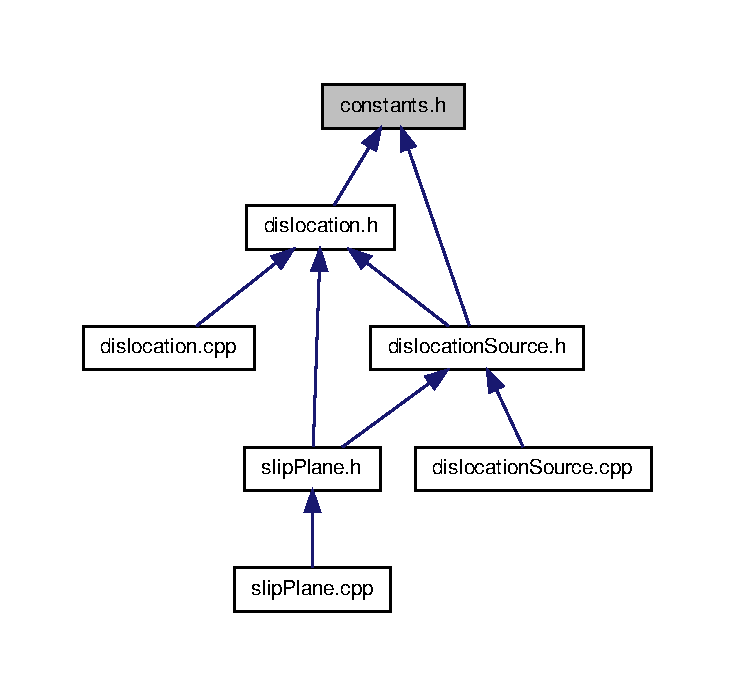
\includegraphics[width=350pt]{dd/d0e/constants_8h__dep__incl}
\end{center}
\end{figure}
\subsection*{Macros}
\begin{DoxyCompactItemize}
\item 
\#define \hyperlink{constants_8h_a598a3330b3c21701223ee0ca14316eca}{P\-I}~3.\-141592654
\begin{DoxyCompactList}\small\item\em The irrational number pi. \end{DoxyCompactList}\item 
\#define \hyperlink{constants_8h_a514396dd60fa0621c83072091fb2a0cd}{S\-Q\-R\-T2}~1.\-414213562
\begin{DoxyCompactList}\small\item\em The square root of 2. \end{DoxyCompactList}\item 
\#define \hyperlink{constants_8h_ae42978afd835c3a1f70d409a1b5f5a39}{S\-Q\-R\-T3}~1.\-732050808
\begin{DoxyCompactList}\small\item\em The square root of 3. \end{DoxyCompactList}\item 
\#define \hyperlink{constants_8h_a9096473cd4539c628de1fa47d919ef78}{S\-Q\-R\-T5}~2.\-236067978
\begin{DoxyCompactList}\small\item\em The square root of 5. \end{DoxyCompactList}\end{DoxyCompactItemize}


\subsection{Detailed Description}
Definition of constants used in the program. \begin{DoxyAuthor}{Author}
Adhish Majumdar 
\end{DoxyAuthor}
\begin{DoxyVersion}{Version}
0.\-0 
\end{DoxyVersion}
\begin{DoxyDate}{Date}
26/04/2013
\end{DoxyDate}
This file defines the values of various constants used in the program. 

Definition in file \hyperlink{constants_8h_source}{constants.\-h}.



\subsection{Macro Definition Documentation}
\hypertarget{constants_8h_a598a3330b3c21701223ee0ca14316eca}{\index{constants.\-h@{constants.\-h}!P\-I@{P\-I}}
\index{P\-I@{P\-I}!constants.h@{constants.\-h}}
\subsubsection[{P\-I}]{\setlength{\rightskip}{0pt plus 5cm}\#define P\-I~3.\-141592654}}\label{d2/d6f/constants_8h_a598a3330b3c21701223ee0ca14316eca}


The irrational number pi. 



Definition at line 16 of file constants.\-h.

\hypertarget{constants_8h_a514396dd60fa0621c83072091fb2a0cd}{\index{constants.\-h@{constants.\-h}!S\-Q\-R\-T2@{S\-Q\-R\-T2}}
\index{S\-Q\-R\-T2@{S\-Q\-R\-T2}!constants.h@{constants.\-h}}
\subsubsection[{S\-Q\-R\-T2}]{\setlength{\rightskip}{0pt plus 5cm}\#define S\-Q\-R\-T2~1.\-414213562}}\label{d2/d6f/constants_8h_a514396dd60fa0621c83072091fb2a0cd}


The square root of 2. 



Definition at line 21 of file constants.\-h.

\hypertarget{constants_8h_ae42978afd835c3a1f70d409a1b5f5a39}{\index{constants.\-h@{constants.\-h}!S\-Q\-R\-T3@{S\-Q\-R\-T3}}
\index{S\-Q\-R\-T3@{S\-Q\-R\-T3}!constants.h@{constants.\-h}}
\subsubsection[{S\-Q\-R\-T3}]{\setlength{\rightskip}{0pt plus 5cm}\#define S\-Q\-R\-T3~1.\-732050808}}\label{d2/d6f/constants_8h_ae42978afd835c3a1f70d409a1b5f5a39}


The square root of 3. 



Definition at line 26 of file constants.\-h.

\hypertarget{constants_8h_a9096473cd4539c628de1fa47d919ef78}{\index{constants.\-h@{constants.\-h}!S\-Q\-R\-T5@{S\-Q\-R\-T5}}
\index{S\-Q\-R\-T5@{S\-Q\-R\-T5}!constants.h@{constants.\-h}}
\subsubsection[{S\-Q\-R\-T5}]{\setlength{\rightskip}{0pt plus 5cm}\#define S\-Q\-R\-T5~2.\-236067978}}\label{d2/d6f/constants_8h_a9096473cd4539c628de1fa47d919ef78}


The square root of 5. 



Definition at line 31 of file constants.\-h.


\hypertarget{defect_8cpp}{\section{defect.\-cpp \-File \-Reference}
\label{dd/def/defect_8cpp}\index{defect.\-cpp@{defect.\-cpp}}
}


\-Definition of member functions of the \hyperlink{classDefect}{\-Defect} class.  


{\ttfamily \#include \char`\"{}defect.\-h\char`\"{}}\*
\-Include dependency graph for defect.\-cpp\-:
\nopagebreak
\begin{figure}[H]
\begin{center}
\leavevmode
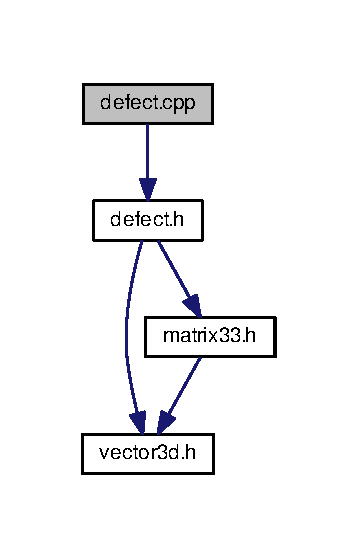
\includegraphics[width=200pt]{dd/dcf/defect_8cpp__incl}
\end{center}
\end{figure}


\subsection{\-Detailed \-Description}
\-Definition of member functions of the \hyperlink{classDefect}{\-Defect} class. \begin{DoxyAuthor}{\-Author}
\-Adhish \-Majumdar 
\end{DoxyAuthor}
\begin{DoxyVersion}{\-Version}
0.\-0 
\end{DoxyVersion}
\begin{DoxyDate}{\-Date}
22/04/2013
\end{DoxyDate}
\-This file defines the member functions of the \hyperlink{classDefect}{\-Defect} class representing a single defect in the simulation. 

\-Definition in file \hyperlink{defect_8cpp_source}{defect.\-cpp}.


\hypertarget{defect_8h}{\section{defect.\-h \-File \-Reference}
\label{df/d55/defect_8h}\index{defect.\-h@{defect.\-h}}
}


\-Definition of the \hyperlink{classDefect}{\-Defect} class.  


{\ttfamily \#include \char`\"{}vector3d.\-h\char`\"{}}\*
{\ttfamily \#include \char`\"{}matrix33.\-h\char`\"{}}\*
{\ttfamily \#include \char`\"{}stress.\-h\char`\"{}}\*
\-Include dependency graph for defect.\-h\-:\nopagebreak
\begin{figure}[H]
\begin{center}
\leavevmode
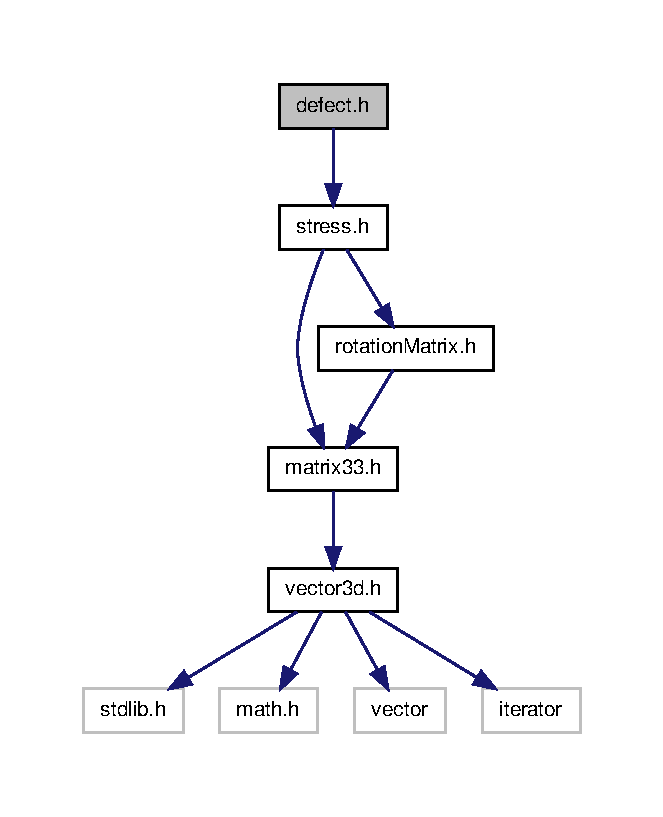
\includegraphics[width=256pt]{d2/d68/defect_8h__incl}
\end{center}
\end{figure}
\-This graph shows which files directly or indirectly include this file\-:\nopagebreak
\begin{figure}[H]
\begin{center}
\leavevmode
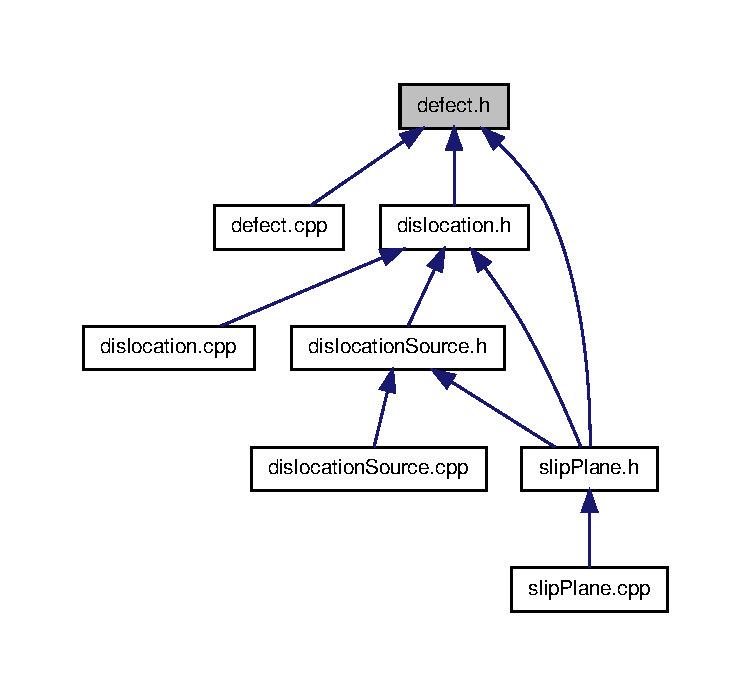
\includegraphics[width=230pt]{dc/d4d/defect_8h__dep__incl}
\end{center}
\end{figure}
\subsection*{\-Data \-Structures}
\begin{DoxyCompactItemize}
\item 
class \hyperlink{classDefect}{\-Defect}
\begin{DoxyCompactList}\small\item\em \-Class \hyperlink{classDefect}{\-Defect} representing a generic defect in a material. \end{DoxyCompactList}\end{DoxyCompactItemize}


\subsection{\-Detailed \-Description}
\-Definition of the \hyperlink{classDefect}{\-Defect} class. \begin{DoxyAuthor}{\-Author}
\-Adhish \-Majumdar 
\end{DoxyAuthor}
\begin{DoxyVersion}{\-Version}
0.\-0 
\end{DoxyVersion}
\begin{DoxyDate}{\-Date}
22/04/2013
\end{DoxyDate}
\-This file defines the \hyperlink{classDefect}{\-Defect} class representing an defect in the simulation. \-This is simply a generic description class with virtual functions. \-Later classes like dislocations, precipitates, boundaries etc will inherit from this class. 

\-Definition in file \hyperlink{defect_8h_source}{defect.\-h}.


\hypertarget{dislocation_8cpp}{\section{dislocation.\-cpp File Reference}
\label{d3/d7f/dislocation_8cpp}\index{dislocation.\-cpp@{dislocation.\-cpp}}
}


Definition of constructors and member functions of the \hyperlink{classDislocation}{Dislocation} class.  


{\ttfamily \#include \char`\"{}dislocation.\-h\char`\"{}}\\*
Include dependency graph for dislocation.\-cpp\-:\nopagebreak
\begin{figure}[H]
\begin{center}
\leavevmode
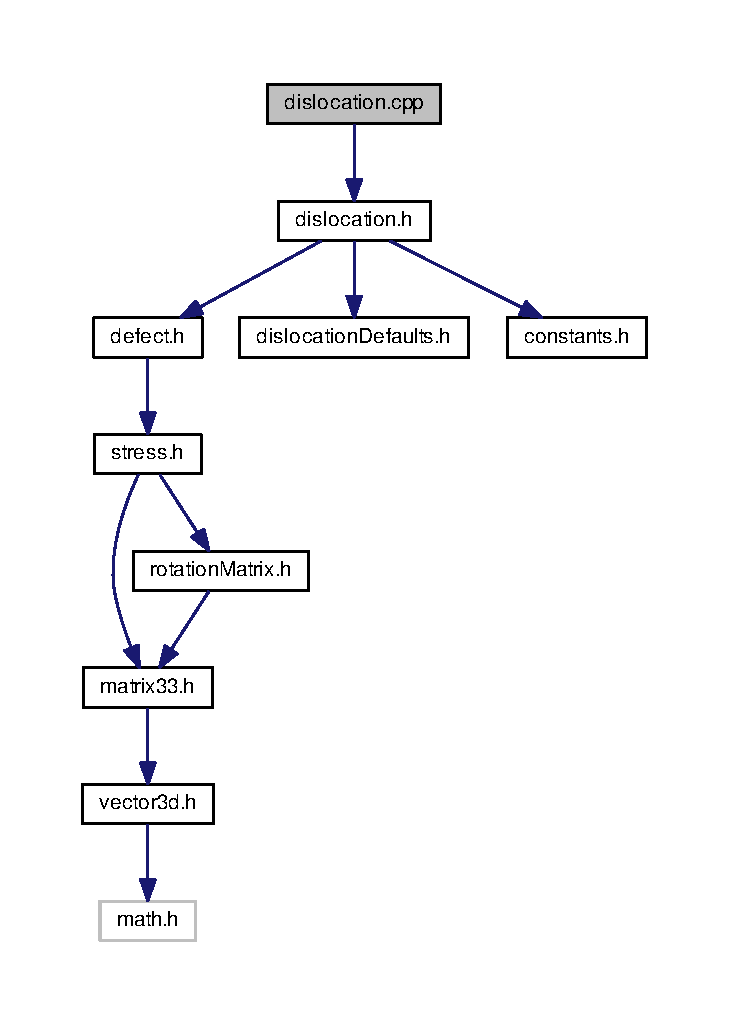
\includegraphics[width=350pt]{d2/d80/dislocation_8cpp__incl}
\end{center}
\end{figure}


\subsection{Detailed Description}
Definition of constructors and member functions of the \hyperlink{classDislocation}{Dislocation} class. \begin{DoxyAuthor}{Author}
Adhish Majumdar 
\end{DoxyAuthor}
\begin{DoxyVersion}{Version}
0.\-0 
\end{DoxyVersion}
\begin{DoxyDate}{Date}
29/04/2013
\end{DoxyDate}
This file defines the constructors and member functions of the \hyperlink{classDislocation}{Dislocation} class. This class inherits from the \hyperlink{classDefect}{Defect} class. 

Definition in file \hyperlink{dislocation_8cpp_source}{dislocation.\-cpp}.


\hypertarget{dislocation_8h}{\section{dislocation.\-h File Reference}
\label{de/df3/dislocation_8h}\index{dislocation.\-h@{dislocation.\-h}}
}


Definition of the \hyperlink{classDislocation}{Dislocation} class.  


{\ttfamily \#include \char`\"{}defect.\-h\char`\"{}}\\*
{\ttfamily \#include \char`\"{}dislocation\-Defaults.\-h\char`\"{}}\\*
{\ttfamily \#include \char`\"{}constants.\-h\char`\"{}}\\*
Include dependency graph for dislocation.\-h\-:\nopagebreak
\begin{figure}[H]
\begin{center}
\leavevmode
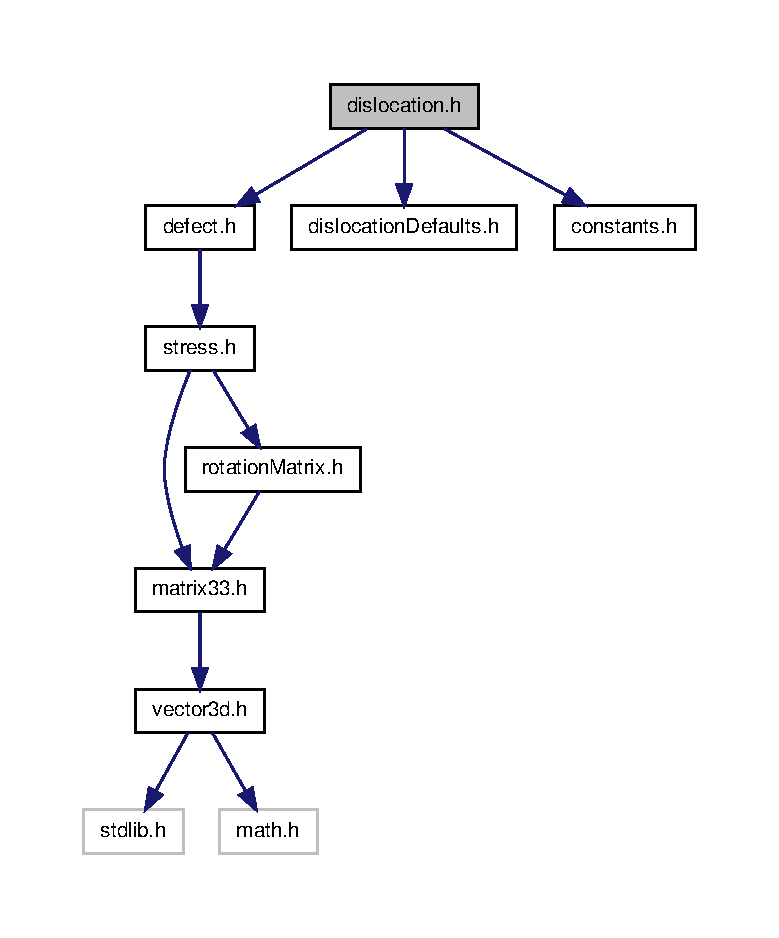
\includegraphics[width=350pt]{dc/dd3/dislocation_8h__incl}
\end{center}
\end{figure}
This graph shows which files directly or indirectly include this file\-:\nopagebreak
\begin{figure}[H]
\begin{center}
\leavevmode
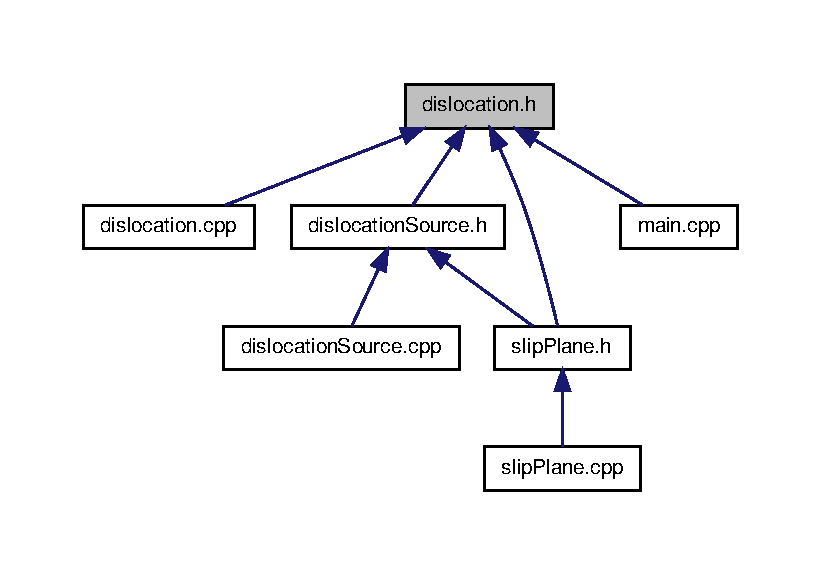
\includegraphics[width=347pt]{dd/d31/dislocation_8h__dep__incl}
\end{center}
\end{figure}
\subsection*{Data Structures}
\begin{DoxyCompactItemize}
\item 
class \hyperlink{classDislocation}{Dislocation}
\begin{DoxyCompactList}\small\item\em \hyperlink{classDislocation}{Dislocation} class representing a dislocation in the simulation. \end{DoxyCompactList}\end{DoxyCompactItemize}
\subsection*{Functions}
\begin{DoxyCompactItemize}
\item 
double \hyperlink{dislocation_8h_ab79ff28442fea06055020a2bba087f78}{ideal\-Time\-Increment} (\hyperlink{classVector3d}{Vector3d} v0, double min\-Distance, \hyperlink{classDefect}{Defect} d, \hyperlink{classVector3d}{Vector3d} v1)
\begin{DoxyCompactList}\small\item\em Returns the ideal time increment for the dislocation. \end{DoxyCompactList}\end{DoxyCompactItemize}


\subsection{Detailed Description}
Definition of the \hyperlink{classDislocation}{Dislocation} class. \begin{DoxyAuthor}{Author}
Adhish Majumdar 
\end{DoxyAuthor}
\begin{DoxyVersion}{Version}
0.\-0 
\end{DoxyVersion}
\begin{DoxyDate}{Date}
03/06/2013
\end{DoxyDate}
This file defines the \hyperlink{classDislocation}{Dislocation} class representing a dislocation in the simulation. This class inherits from the \hyperlink{classDefect}{Defect} class. 

Definition in file \hyperlink{dislocation_8h_source}{dislocation.\-h}.



\subsection{Function Documentation}
\hypertarget{dislocation_8h_ab79ff28442fea06055020a2bba087f78}{\index{dislocation.\-h@{dislocation.\-h}!ideal\-Time\-Increment@{ideal\-Time\-Increment}}
\index{ideal\-Time\-Increment@{ideal\-Time\-Increment}!dislocation.h@{dislocation.\-h}}
\subsubsection[{ideal\-Time\-Increment}]{\setlength{\rightskip}{0pt plus 5cm}double Dislocation\-::ideal\-Time\-Increment (
\begin{DoxyParamCaption}
\item[{{\bf Vector3d}}]{v0, }
\item[{double}]{min\-Distance, }
\item[{{\bf Defect}}]{d, }
\item[{{\bf Vector3d}}]{v1}
\end{DoxyParamCaption}
)}}\label{de/df3/dislocation_8h_ab79ff28442fea06055020a2bba087f78}


Returns the ideal time increment for the dislocation. 

A dislocation is not allowed to approach another dislocation of equal sign beyond a certain distance, specified by the argument min\-Distance. This function calculates the ideal time increment for this dislocation to not collide with another dislocation. 
\begin{DoxyParams}{Parameters}
{\em v0} & Velocity of the dislocation. \\
\hline
{\em min\-Distance} & Minimum distance of approach to the dislocation. \\
\hline
{\em d} & The defect for which the present dislocation's time increment is to be calculated. \\
\hline
{\em v1} & Velocity of the other defect. \\
\hline
\end{DoxyParams}
\begin{DoxyReturn}{Returns}
The ideal time increment for this dislocation. 
\end{DoxyReturn}


Definition at line 225 of file dislocation.\-cpp.


\begin{DoxyCode}
226 \{
227   \textcolor{keywordtype}{double} norm\_v0 = v0.\hyperlink{classVector3d_a9fd3cba8bbdf983db6c2a2eae00c4b29}{magnitude}();
228   \textcolor{keywordflow}{if} (norm\_v0 == 0.0)
229     \{
230       \textcolor{comment}{// This dislocation is not moving}
231       \textcolor{keywordflow}{return} (1000.0);
232     \}
233 
234   \textcolor{comment}{// Positions}
235   \hyperlink{classVector3d}{Vector3d} p0 = this->getPosition();
236   \hyperlink{classVector3d}{Vector3d} p1 = d.\hyperlink{classDefect_a270caed3561fa5fa284af6427b6ca2e4}{getPosition}();
237   \hyperlink{classVector3d}{Vector3d} p01 = p1 - p0;
238   \textcolor{keywordtype}{double} norm\_p01 = p01.\hyperlink{classVector3d_a9fd3cba8bbdf983db6c2a2eae00c4b29}{magnitude}();
239 
240   \textcolor{keywordflow}{if} (norm\_p01 == 0.0)
241     \{
242       \textcolor{comment}{// The dislocation is lying on top of the obstacle - so it should not move}
243       \textcolor{keywordflow}{return} (0.0);
244     \}
245   \textcolor{keywordflow}{else}
246     \{
247       \textcolor{comment}{// Find out if the dislocation is approaching the defect or not}
248 
249       \textcolor{comment}{// Velocities}
250       \hyperlink{classVector3d}{Vector3d} v01 = v1 - v0;
251       \textcolor{keywordtype}{double} norm\_v01 = v01.\hyperlink{classVector3d_a9fd3cba8bbdf983db6c2a2eae00c4b29}{magnitude}();
252       \textcolor{keywordtype}{double} dotProduct = v01 * p01;
253       \textcolor{keywordtype}{double} cosine = dotProduct/(norm\_v01 * norm\_p01);
254       \textcolor{keywordflow}{if} (cosine < 0.0)
255         \{
256           \textcolor{comment}{// The dislocation is approaching the other defect}
257           \textcolor{keywordflow}{return} ( (norm\_p01 - minDistance)/norm\_v01 );
258         \}
259       \textcolor{keywordflow}{else}
260         \{
261           \textcolor{comment}{// They are diverging}
262           \textcolor{comment}{// So any time increment will do}
263           \textcolor{keywordflow}{return} (1000.0);
264         \}
265     \}
266 \}
\end{DoxyCode}

\hypertarget{dislocationDefaults_8h}{\section{dislocation\-Defaults.\-h \-File \-Reference}
\label{d4/da6/dislocationDefaults_8h}\index{dislocation\-Defaults.\-h@{dislocation\-Defaults.\-h}}
}


\-Definition of certain default values for members of the \hyperlink{classDislocation}{\-Dislocation} class.  


\-This graph shows which files directly or indirectly include this file\-:
\nopagebreak
\begin{figure}[H]
\begin{center}
\leavevmode
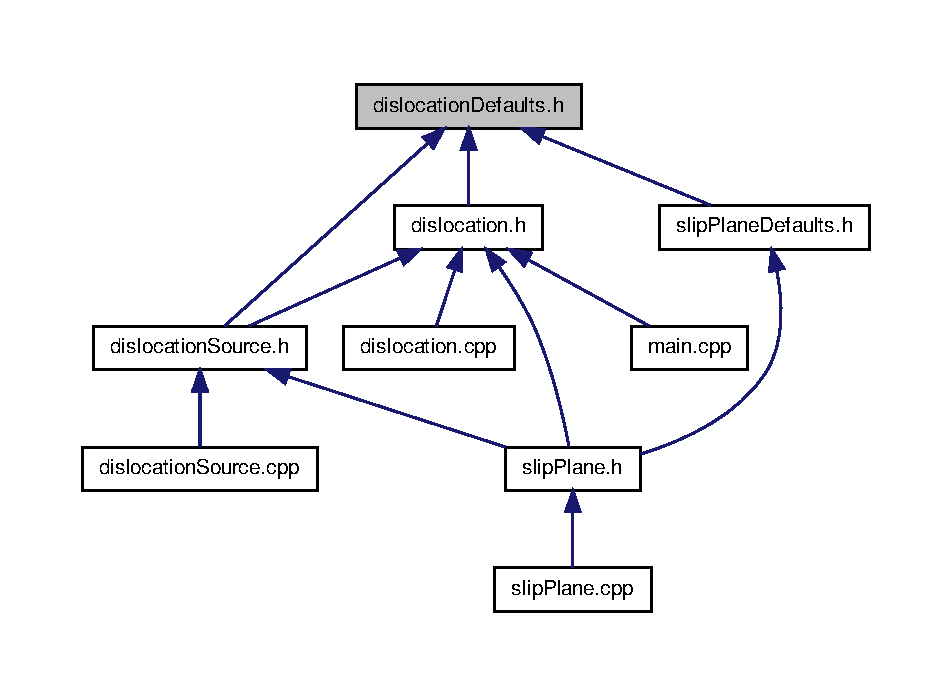
\includegraphics[width=350pt]{d0/dcc/dislocationDefaults_8h__dep__incl}
\end{center}
\end{figure}
\subsection*{\-Defines}
\begin{DoxyCompactItemize}
\item 
\#define \hyperlink{dislocationDefaults_8h_a797caa5c52e49fd8d7db6af9bceea257}{\-D\-E\-F\-A\-U\-L\-T\-\_\-\-P\-O\-S\-I\-T\-I\-O\-N\-\_\-0}~0.\-0
\begin{DoxyCompactList}\small\item\em \-Default value of the position vector x-\/coordinate. \end{DoxyCompactList}\item 
\#define \hyperlink{dislocationDefaults_8h_a88a33ddda5bafb85a662e09f9cf28e6d}{\-D\-E\-F\-A\-U\-L\-T\-\_\-\-P\-O\-S\-I\-T\-I\-O\-N\-\_\-1}~0.\-0
\begin{DoxyCompactList}\small\item\em \-Default value of the position vector y-\/coordinate. \end{DoxyCompactList}\item 
\#define \hyperlink{dislocationDefaults_8h_ad61c6c206e346b3f239c0bba69773eeb}{\-D\-E\-F\-A\-U\-L\-T\-\_\-\-P\-O\-S\-I\-T\-I\-O\-N\-\_\-2}~0.\-0
\begin{DoxyCompactList}\small\item\em \-Default value of the position vector z-\/coordinate. \end{DoxyCompactList}\item 
\#define \hyperlink{dislocationDefaults_8h_a48b2523eeb3e024b79124f9f4c50004b}{\-D\-E\-F\-A\-U\-L\-T\-\_\-\-B\-U\-R\-G\-E\-R\-S\-\_\-\-M\-A\-G\-N\-I\-T\-U\-D\-E}~5.\-0e-\/09
\begin{DoxyCompactList}\small\item\em \-Default value of the magnitude of the \-Burgers vector. \end{DoxyCompactList}\item 
\#define \hyperlink{dislocationDefaults_8h_a8bc0403713fea52c48652247734ed060}{\-D\-E\-F\-A\-U\-L\-T\-\_\-\-B\-U\-R\-G\-E\-R\-S\-\_\-0}~1.\-0
\begin{DoxyCompactList}\small\item\em \-Default value of the \-Burgers vector x-\/coordinate. \end{DoxyCompactList}\item 
\#define \hyperlink{dislocationDefaults_8h_a77a5b4d23da175ef84909c513649d6bf}{\-D\-E\-F\-A\-U\-L\-T\-\_\-\-B\-U\-R\-G\-E\-R\-S\-\_\-1}~1.\-0
\begin{DoxyCompactList}\small\item\em \-Default value of the \-Burgers vector y-\/coordinate. \end{DoxyCompactList}\item 
\#define \hyperlink{dislocationDefaults_8h_a340578d3def7d31536ca2ae4ae444ee1}{\-D\-E\-F\-A\-U\-L\-T\-\_\-\-B\-U\-R\-G\-E\-R\-S\-\_\-2}~0.\-0
\begin{DoxyCompactList}\small\item\em \-Default value of the \-Burgers vector z-\/coordinate. \end{DoxyCompactList}\item 
\#define \hyperlink{dislocationDefaults_8h_a3969abd5a63f951f079c148314416bd2}{\-D\-E\-F\-A\-U\-L\-T\-\_\-\-L\-I\-N\-E\-V\-E\-C\-T\-O\-R\-\_\-0}~1.\-0
\begin{DoxyCompactList}\small\item\em \-Default value of the line vector x-\/coordinate. \end{DoxyCompactList}\item 
\#define \hyperlink{dislocationDefaults_8h_a5d1040038b6cc2afcdf3f935785a118b}{\-D\-E\-F\-A\-U\-L\-T\-\_\-\-L\-I\-N\-E\-V\-E\-C\-T\-O\-R\-\_\-1}~-\/1.\-0
\begin{DoxyCompactList}\small\item\em \-Default value of the line vector y-\/coordinate. \end{DoxyCompactList}\item 
\#define \hyperlink{dislocationDefaults_8h_a517bab607d45c13734cc8450a1062b1d}{\-D\-E\-F\-A\-U\-L\-T\-\_\-\-L\-I\-N\-E\-V\-E\-C\-T\-O\-R\-\_\-2}~-\/2.\-0
\begin{DoxyCompactList}\small\item\em \-Default value of the line vector z-\/coordinate. \end{DoxyCompactList}\end{DoxyCompactItemize}


\subsection{\-Detailed \-Description}
\-Definition of certain default values for members of the \hyperlink{classDislocation}{\-Dislocation} class. \begin{DoxyAuthor}{\-Author}
\-Adhish \-Majumdar 
\end{DoxyAuthor}
\begin{DoxyVersion}{\-Version}
0.\-0 
\end{DoxyVersion}
\begin{DoxyDate}{\-Date}
26/04/2013
\end{DoxyDate}
\-This file defines some default values for members of the \hyperlink{classDislocation}{\-Dislocation} class representing a dislocation in the simulation. 

\-Definition in file \hyperlink{dislocationDefaults_8h_source}{dislocation\-Defaults.\-h}.



\subsection{\-Define \-Documentation}
\hypertarget{dislocationDefaults_8h_a8bc0403713fea52c48652247734ed060}{\index{dislocation\-Defaults.\-h@{dislocation\-Defaults.\-h}!\-D\-E\-F\-A\-U\-L\-T\-\_\-\-B\-U\-R\-G\-E\-R\-S\-\_\-0@{\-D\-E\-F\-A\-U\-L\-T\-\_\-\-B\-U\-R\-G\-E\-R\-S\-\_\-0}}
\index{\-D\-E\-F\-A\-U\-L\-T\-\_\-\-B\-U\-R\-G\-E\-R\-S\-\_\-0@{\-D\-E\-F\-A\-U\-L\-T\-\_\-\-B\-U\-R\-G\-E\-R\-S\-\_\-0}!dislocationDefaults.h@{dislocation\-Defaults.\-h}}
\subsubsection[{\-D\-E\-F\-A\-U\-L\-T\-\_\-\-B\-U\-R\-G\-E\-R\-S\-\_\-0}]{\setlength{\rightskip}{0pt plus 5cm}\#define {\bf \-D\-E\-F\-A\-U\-L\-T\-\_\-\-B\-U\-R\-G\-E\-R\-S\-\_\-0}~1.\-0}}\label{d4/da6/dislocationDefaults_8h_a8bc0403713fea52c48652247734ed060}


\-Default value of the \-Burgers vector x-\/coordinate. 



\-Definition at line 34 of file dislocation\-Defaults.\-h.

\hypertarget{dislocationDefaults_8h_a77a5b4d23da175ef84909c513649d6bf}{\index{dislocation\-Defaults.\-h@{dislocation\-Defaults.\-h}!\-D\-E\-F\-A\-U\-L\-T\-\_\-\-B\-U\-R\-G\-E\-R\-S\-\_\-1@{\-D\-E\-F\-A\-U\-L\-T\-\_\-\-B\-U\-R\-G\-E\-R\-S\-\_\-1}}
\index{\-D\-E\-F\-A\-U\-L\-T\-\_\-\-B\-U\-R\-G\-E\-R\-S\-\_\-1@{\-D\-E\-F\-A\-U\-L\-T\-\_\-\-B\-U\-R\-G\-E\-R\-S\-\_\-1}!dislocationDefaults.h@{dislocation\-Defaults.\-h}}
\subsubsection[{\-D\-E\-F\-A\-U\-L\-T\-\_\-\-B\-U\-R\-G\-E\-R\-S\-\_\-1}]{\setlength{\rightskip}{0pt plus 5cm}\#define {\bf \-D\-E\-F\-A\-U\-L\-T\-\_\-\-B\-U\-R\-G\-E\-R\-S\-\_\-1}~1.\-0}}\label{d4/da6/dislocationDefaults_8h_a77a5b4d23da175ef84909c513649d6bf}


\-Default value of the \-Burgers vector y-\/coordinate. 



\-Definition at line 38 of file dislocation\-Defaults.\-h.

\hypertarget{dislocationDefaults_8h_a340578d3def7d31536ca2ae4ae444ee1}{\index{dislocation\-Defaults.\-h@{dislocation\-Defaults.\-h}!\-D\-E\-F\-A\-U\-L\-T\-\_\-\-B\-U\-R\-G\-E\-R\-S\-\_\-2@{\-D\-E\-F\-A\-U\-L\-T\-\_\-\-B\-U\-R\-G\-E\-R\-S\-\_\-2}}
\index{\-D\-E\-F\-A\-U\-L\-T\-\_\-\-B\-U\-R\-G\-E\-R\-S\-\_\-2@{\-D\-E\-F\-A\-U\-L\-T\-\_\-\-B\-U\-R\-G\-E\-R\-S\-\_\-2}!dislocationDefaults.h@{dislocation\-Defaults.\-h}}
\subsubsection[{\-D\-E\-F\-A\-U\-L\-T\-\_\-\-B\-U\-R\-G\-E\-R\-S\-\_\-2}]{\setlength{\rightskip}{0pt plus 5cm}\#define {\bf \-D\-E\-F\-A\-U\-L\-T\-\_\-\-B\-U\-R\-G\-E\-R\-S\-\_\-2}~0.\-0}}\label{d4/da6/dislocationDefaults_8h_a340578d3def7d31536ca2ae4ae444ee1}


\-Default value of the \-Burgers vector z-\/coordinate. 



\-Definition at line 42 of file dislocation\-Defaults.\-h.

\hypertarget{dislocationDefaults_8h_a48b2523eeb3e024b79124f9f4c50004b}{\index{dislocation\-Defaults.\-h@{dislocation\-Defaults.\-h}!\-D\-E\-F\-A\-U\-L\-T\-\_\-\-B\-U\-R\-G\-E\-R\-S\-\_\-\-M\-A\-G\-N\-I\-T\-U\-D\-E@{\-D\-E\-F\-A\-U\-L\-T\-\_\-\-B\-U\-R\-G\-E\-R\-S\-\_\-\-M\-A\-G\-N\-I\-T\-U\-D\-E}}
\index{\-D\-E\-F\-A\-U\-L\-T\-\_\-\-B\-U\-R\-G\-E\-R\-S\-\_\-\-M\-A\-G\-N\-I\-T\-U\-D\-E@{\-D\-E\-F\-A\-U\-L\-T\-\_\-\-B\-U\-R\-G\-E\-R\-S\-\_\-\-M\-A\-G\-N\-I\-T\-U\-D\-E}!dislocationDefaults.h@{dislocation\-Defaults.\-h}}
\subsubsection[{\-D\-E\-F\-A\-U\-L\-T\-\_\-\-B\-U\-R\-G\-E\-R\-S\-\_\-\-M\-A\-G\-N\-I\-T\-U\-D\-E}]{\setlength{\rightskip}{0pt plus 5cm}\#define {\bf \-D\-E\-F\-A\-U\-L\-T\-\_\-\-B\-U\-R\-G\-E\-R\-S\-\_\-\-M\-A\-G\-N\-I\-T\-U\-D\-E}~5.\-0e-\/09}}\label{d4/da6/dislocationDefaults_8h_a48b2523eeb3e024b79124f9f4c50004b}


\-Default value of the magnitude of the \-Burgers vector. 



\-Definition at line 29 of file dislocation\-Defaults.\-h.

\hypertarget{dislocationDefaults_8h_a3969abd5a63f951f079c148314416bd2}{\index{dislocation\-Defaults.\-h@{dislocation\-Defaults.\-h}!\-D\-E\-F\-A\-U\-L\-T\-\_\-\-L\-I\-N\-E\-V\-E\-C\-T\-O\-R\-\_\-0@{\-D\-E\-F\-A\-U\-L\-T\-\_\-\-L\-I\-N\-E\-V\-E\-C\-T\-O\-R\-\_\-0}}
\index{\-D\-E\-F\-A\-U\-L\-T\-\_\-\-L\-I\-N\-E\-V\-E\-C\-T\-O\-R\-\_\-0@{\-D\-E\-F\-A\-U\-L\-T\-\_\-\-L\-I\-N\-E\-V\-E\-C\-T\-O\-R\-\_\-0}!dislocationDefaults.h@{dislocation\-Defaults.\-h}}
\subsubsection[{\-D\-E\-F\-A\-U\-L\-T\-\_\-\-L\-I\-N\-E\-V\-E\-C\-T\-O\-R\-\_\-0}]{\setlength{\rightskip}{0pt plus 5cm}\#define {\bf \-D\-E\-F\-A\-U\-L\-T\-\_\-\-L\-I\-N\-E\-V\-E\-C\-T\-O\-R\-\_\-0}~1.\-0}}\label{d4/da6/dislocationDefaults_8h_a3969abd5a63f951f079c148314416bd2}


\-Default value of the line vector x-\/coordinate. 



\-Definition at line 47 of file dislocation\-Defaults.\-h.

\hypertarget{dislocationDefaults_8h_a5d1040038b6cc2afcdf3f935785a118b}{\index{dislocation\-Defaults.\-h@{dislocation\-Defaults.\-h}!\-D\-E\-F\-A\-U\-L\-T\-\_\-\-L\-I\-N\-E\-V\-E\-C\-T\-O\-R\-\_\-1@{\-D\-E\-F\-A\-U\-L\-T\-\_\-\-L\-I\-N\-E\-V\-E\-C\-T\-O\-R\-\_\-1}}
\index{\-D\-E\-F\-A\-U\-L\-T\-\_\-\-L\-I\-N\-E\-V\-E\-C\-T\-O\-R\-\_\-1@{\-D\-E\-F\-A\-U\-L\-T\-\_\-\-L\-I\-N\-E\-V\-E\-C\-T\-O\-R\-\_\-1}!dislocationDefaults.h@{dislocation\-Defaults.\-h}}
\subsubsection[{\-D\-E\-F\-A\-U\-L\-T\-\_\-\-L\-I\-N\-E\-V\-E\-C\-T\-O\-R\-\_\-1}]{\setlength{\rightskip}{0pt plus 5cm}\#define {\bf \-D\-E\-F\-A\-U\-L\-T\-\_\-\-L\-I\-N\-E\-V\-E\-C\-T\-O\-R\-\_\-1}~-\/1.\-0}}\label{d4/da6/dislocationDefaults_8h_a5d1040038b6cc2afcdf3f935785a118b}


\-Default value of the line vector y-\/coordinate. 



\-Definition at line 51 of file dislocation\-Defaults.\-h.

\hypertarget{dislocationDefaults_8h_a517bab607d45c13734cc8450a1062b1d}{\index{dislocation\-Defaults.\-h@{dislocation\-Defaults.\-h}!\-D\-E\-F\-A\-U\-L\-T\-\_\-\-L\-I\-N\-E\-V\-E\-C\-T\-O\-R\-\_\-2@{\-D\-E\-F\-A\-U\-L\-T\-\_\-\-L\-I\-N\-E\-V\-E\-C\-T\-O\-R\-\_\-2}}
\index{\-D\-E\-F\-A\-U\-L\-T\-\_\-\-L\-I\-N\-E\-V\-E\-C\-T\-O\-R\-\_\-2@{\-D\-E\-F\-A\-U\-L\-T\-\_\-\-L\-I\-N\-E\-V\-E\-C\-T\-O\-R\-\_\-2}!dislocationDefaults.h@{dislocation\-Defaults.\-h}}
\subsubsection[{\-D\-E\-F\-A\-U\-L\-T\-\_\-\-L\-I\-N\-E\-V\-E\-C\-T\-O\-R\-\_\-2}]{\setlength{\rightskip}{0pt plus 5cm}\#define {\bf \-D\-E\-F\-A\-U\-L\-T\-\_\-\-L\-I\-N\-E\-V\-E\-C\-T\-O\-R\-\_\-2}~-\/2.\-0}}\label{d4/da6/dislocationDefaults_8h_a517bab607d45c13734cc8450a1062b1d}


\-Default value of the line vector z-\/coordinate. 



\-Definition at line 55 of file dislocation\-Defaults.\-h.

\hypertarget{dislocationDefaults_8h_a797caa5c52e49fd8d7db6af9bceea257}{\index{dislocation\-Defaults.\-h@{dislocation\-Defaults.\-h}!\-D\-E\-F\-A\-U\-L\-T\-\_\-\-P\-O\-S\-I\-T\-I\-O\-N\-\_\-0@{\-D\-E\-F\-A\-U\-L\-T\-\_\-\-P\-O\-S\-I\-T\-I\-O\-N\-\_\-0}}
\index{\-D\-E\-F\-A\-U\-L\-T\-\_\-\-P\-O\-S\-I\-T\-I\-O\-N\-\_\-0@{\-D\-E\-F\-A\-U\-L\-T\-\_\-\-P\-O\-S\-I\-T\-I\-O\-N\-\_\-0}!dislocationDefaults.h@{dislocation\-Defaults.\-h}}
\subsubsection[{\-D\-E\-F\-A\-U\-L\-T\-\_\-\-P\-O\-S\-I\-T\-I\-O\-N\-\_\-0}]{\setlength{\rightskip}{0pt plus 5cm}\#define {\bf \-D\-E\-F\-A\-U\-L\-T\-\_\-\-P\-O\-S\-I\-T\-I\-O\-N\-\_\-0}~0.\-0}}\label{d4/da6/dislocationDefaults_8h_a797caa5c52e49fd8d7db6af9bceea257}


\-Default value of the position vector x-\/coordinate. 



\-Definition at line 16 of file dislocation\-Defaults.\-h.

\hypertarget{dislocationDefaults_8h_a88a33ddda5bafb85a662e09f9cf28e6d}{\index{dislocation\-Defaults.\-h@{dislocation\-Defaults.\-h}!\-D\-E\-F\-A\-U\-L\-T\-\_\-\-P\-O\-S\-I\-T\-I\-O\-N\-\_\-1@{\-D\-E\-F\-A\-U\-L\-T\-\_\-\-P\-O\-S\-I\-T\-I\-O\-N\-\_\-1}}
\index{\-D\-E\-F\-A\-U\-L\-T\-\_\-\-P\-O\-S\-I\-T\-I\-O\-N\-\_\-1@{\-D\-E\-F\-A\-U\-L\-T\-\_\-\-P\-O\-S\-I\-T\-I\-O\-N\-\_\-1}!dislocationDefaults.h@{dislocation\-Defaults.\-h}}
\subsubsection[{\-D\-E\-F\-A\-U\-L\-T\-\_\-\-P\-O\-S\-I\-T\-I\-O\-N\-\_\-1}]{\setlength{\rightskip}{0pt plus 5cm}\#define {\bf \-D\-E\-F\-A\-U\-L\-T\-\_\-\-P\-O\-S\-I\-T\-I\-O\-N\-\_\-1}~0.\-0}}\label{d4/da6/dislocationDefaults_8h_a88a33ddda5bafb85a662e09f9cf28e6d}


\-Default value of the position vector y-\/coordinate. 



\-Definition at line 20 of file dislocation\-Defaults.\-h.

\hypertarget{dislocationDefaults_8h_ad61c6c206e346b3f239c0bba69773eeb}{\index{dislocation\-Defaults.\-h@{dislocation\-Defaults.\-h}!\-D\-E\-F\-A\-U\-L\-T\-\_\-\-P\-O\-S\-I\-T\-I\-O\-N\-\_\-2@{\-D\-E\-F\-A\-U\-L\-T\-\_\-\-P\-O\-S\-I\-T\-I\-O\-N\-\_\-2}}
\index{\-D\-E\-F\-A\-U\-L\-T\-\_\-\-P\-O\-S\-I\-T\-I\-O\-N\-\_\-2@{\-D\-E\-F\-A\-U\-L\-T\-\_\-\-P\-O\-S\-I\-T\-I\-O\-N\-\_\-2}!dislocationDefaults.h@{dislocation\-Defaults.\-h}}
\subsubsection[{\-D\-E\-F\-A\-U\-L\-T\-\_\-\-P\-O\-S\-I\-T\-I\-O\-N\-\_\-2}]{\setlength{\rightskip}{0pt plus 5cm}\#define {\bf \-D\-E\-F\-A\-U\-L\-T\-\_\-\-P\-O\-S\-I\-T\-I\-O\-N\-\_\-2}~0.\-0}}\label{d4/da6/dislocationDefaults_8h_ad61c6c206e346b3f239c0bba69773eeb}


\-Default value of the position vector z-\/coordinate. 



\-Definition at line 24 of file dislocation\-Defaults.\-h.


\hypertarget{matrix33_8cpp}{\section{matrix33.\-cpp \-File \-Reference}
\label{d8/d8e/matrix33_8cpp}\index{matrix33.\-cpp@{matrix33.\-cpp}}
}


\-Definition of the member functions and operators of the \hyperlink{classMatrix33}{\-Matrix33} class.  


{\ttfamily \#include \char`\"{}matrix33.\-h\char`\"{}}\*
\-Include dependency graph for matrix33.\-cpp\-:\nopagebreak
\begin{figure}[H]
\begin{center}
\leavevmode
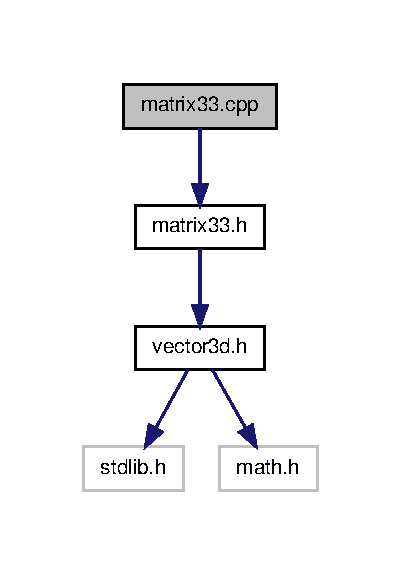
\includegraphics[width=318pt]{d8/d6d/matrix33_8cpp__incl}
\end{center}
\end{figure}


\subsection{\-Detailed \-Description}
\-Definition of the member functions and operators of the \hyperlink{classMatrix33}{\-Matrix33} class. \begin{DoxyAuthor}{\-Author}
\-Adhish \-Majumdar 
\end{DoxyAuthor}
\begin{DoxyVersion}{\-Version}
1.\-0 
\end{DoxyVersion}
\begin{DoxyDate}{\-Date}
04/06/2013
\end{DoxyDate}
\-This file defines the member functions and operators of the \hyperlink{classMatrix33}{\-Matrix33} class representing a 3x3 matrix in the simulation. 

\-Definition in file \hyperlink{matrix33_8cpp_source}{matrix33.\-cpp}.


\hypertarget{matrix33_8h}{\section{matrix33.\-h File Reference}
\label{db/d46/matrix33_8h}\index{matrix33.\-h@{matrix33.\-h}}
}


Definition of the \hyperlink{classMatrix33}{Matrix33} class.  


{\ttfamily \#include \char`\"{}vector3d.\-h\char`\"{}}\\*
Include dependency graph for matrix33.\-h\-:\nopagebreak
\begin{figure}[H]
\begin{center}
\leavevmode
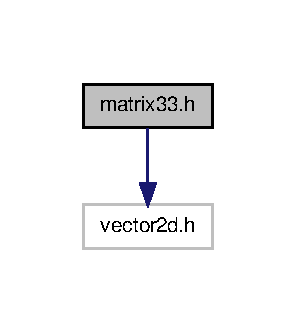
\includegraphics[width=142pt]{d7/dc7/matrix33_8h__incl}
\end{center}
\end{figure}
This graph shows which files directly or indirectly include this file\-:
\nopagebreak
\begin{figure}[H]
\begin{center}
\leavevmode
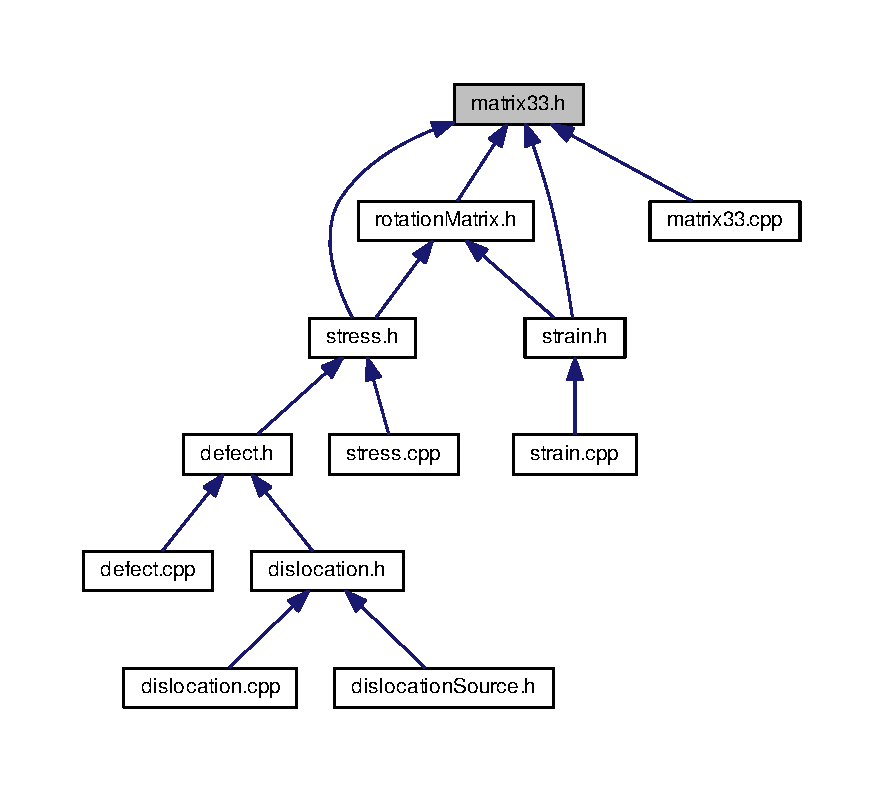
\includegraphics[width=301pt]{dd/d84/matrix33_8h__dep__incl}
\end{center}
\end{figure}
\subsection*{Data Structures}
\begin{DoxyCompactItemize}
\item 
class \hyperlink{classMatrix33}{Matrix33}
\begin{DoxyCompactList}\small\item\em \hyperlink{classMatrix33}{Matrix33} class representing a 3x3 square matrix. \end{DoxyCompactList}\end{DoxyCompactItemize}


\subsection{Detailed Description}
Definition of the \hyperlink{classMatrix33}{Matrix33} class. \begin{DoxyAuthor}{Author}
Adhish Majumdar 
\end{DoxyAuthor}
\begin{DoxyVersion}{Version}
0.\-0 
\end{DoxyVersion}
\begin{DoxyDate}{Date}
22/04/2013
\end{DoxyDate}
This file defines the \hyperlink{classMatrix33}{Matrix33} class representing a 3x3 matrix in the simulation. 

Definition in file \hyperlink{matrix33_8h_source}{matrix33.\-h}.


\hypertarget{rotationMatrix_8cpp}{\section{rotation\-Matrix.\-cpp File Reference}
\label{d9/d5c/rotationMatrix_8cpp}\index{rotation\-Matrix.\-cpp@{rotation\-Matrix.\-cpp}}
}


Definition of the \hyperlink{classRotationMatrix}{Rotation\-Matrix} class member functions.  




\subsection{Detailed Description}
Definition of the \hyperlink{classRotationMatrix}{Rotation\-Matrix} class member functions. \begin{DoxyAuthor}{Author}
Adhish Majumdar 
\end{DoxyAuthor}
\begin{DoxyVersion}{Version}
0.\-0 
\end{DoxyVersion}
\begin{DoxyDate}{Date}
25/04/2013
\end{DoxyDate}
This file defines member functions of the \hyperlink{classRotationMatrix}{Rotation\-Matrix} class for carrying out 3\-D rotations and axes transformations. 

Definition in file \hyperlink{rotationMatrix_8cpp_source}{rotation\-Matrix.\-cpp}.


\hypertarget{rotationMatrix_8h}{\section{rotation\-Matrix.\-h \-File \-Reference}
\label{da/d76/rotationMatrix_8h}\index{rotation\-Matrix.\-h@{rotation\-Matrix.\-h}}
}


\-Definition of the \hyperlink{classRotationMatrix}{\-Rotation\-Matrix} class.  


{\ttfamily \#include \char`\"{}matrix33.\-h\char`\"{}}\*
\-Include dependency graph for rotation\-Matrix.\-h\-:\nopagebreak
\begin{figure}[H]
\begin{center}
\leavevmode
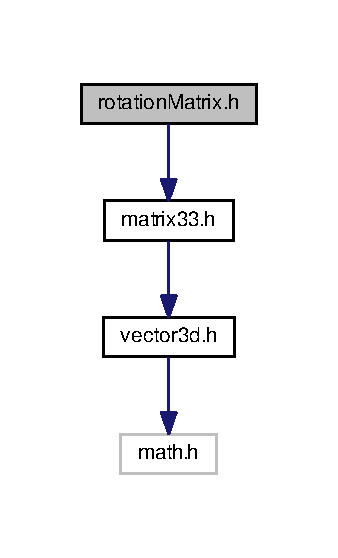
\includegraphics[width=318pt]{dc/d6c/rotationMatrix_8h__incl}
\end{center}
\end{figure}
\-This graph shows which files directly or indirectly include this file\-:
\nopagebreak
\begin{figure}[H]
\begin{center}
\leavevmode
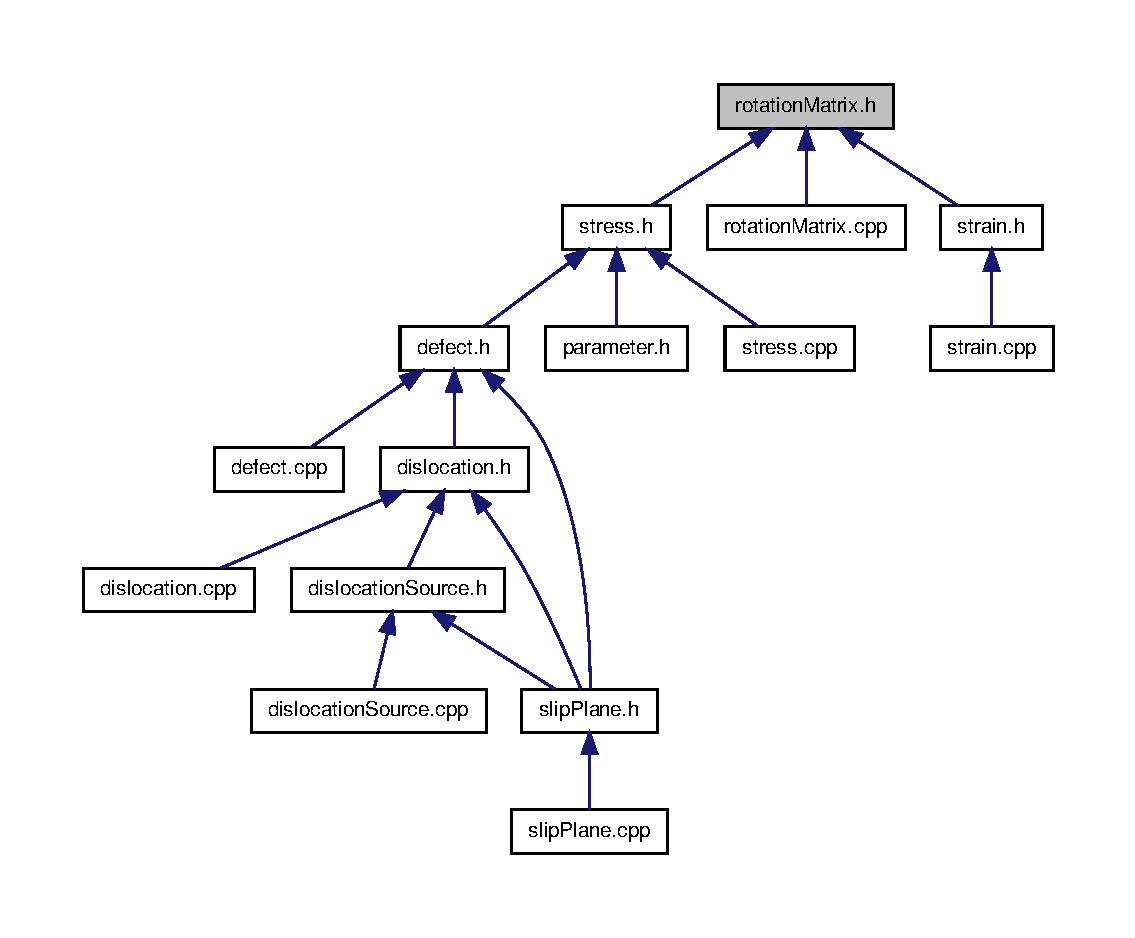
\includegraphics[width=350pt]{dd/da3/rotationMatrix_8h__dep__incl}
\end{center}
\end{figure}
\subsection*{\-Data \-Structures}
\begin{DoxyCompactItemize}
\item 
class \hyperlink{classRotationMatrix}{\-Rotation\-Matrix}
\begin{DoxyCompactList}\small\item\em \hyperlink{classRotationMatrix}{\-Rotation\-Matrix} class to represent a rotation matrix. \end{DoxyCompactList}\end{DoxyCompactItemize}


\subsection{\-Detailed \-Description}
\-Definition of the \hyperlink{classRotationMatrix}{\-Rotation\-Matrix} class. \begin{DoxyAuthor}{\-Author}
\-Adhish \-Majumdar 
\end{DoxyAuthor}
\begin{DoxyVersion}{\-Version}
0.\-0 
\end{DoxyVersion}
\begin{DoxyDate}{\-Date}
25/04/2013
\end{DoxyDate}
\-This file defines the \hyperlink{classRotationMatrix}{\-Rotation\-Matrix} class for carrying out 3\-D rotations and axes transformations. 

\-Definition in file \hyperlink{rotationMatrix_8h_source}{rotation\-Matrix.\-h}.


\hypertarget{strain_8cpp}{\section{strain.\-cpp File Reference}
\label{d7/db1/strain_8cpp}\index{strain.\-cpp@{strain.\-cpp}}
}


Definition of the member functions if the \hyperlink{classStrain}{Strain} class.  


{\ttfamily \#include \char`\"{}strain.\-h\char`\"{}}\\*
Include dependency graph for strain.\-cpp\-:\nopagebreak
\begin{figure}[H]
\begin{center}
\leavevmode
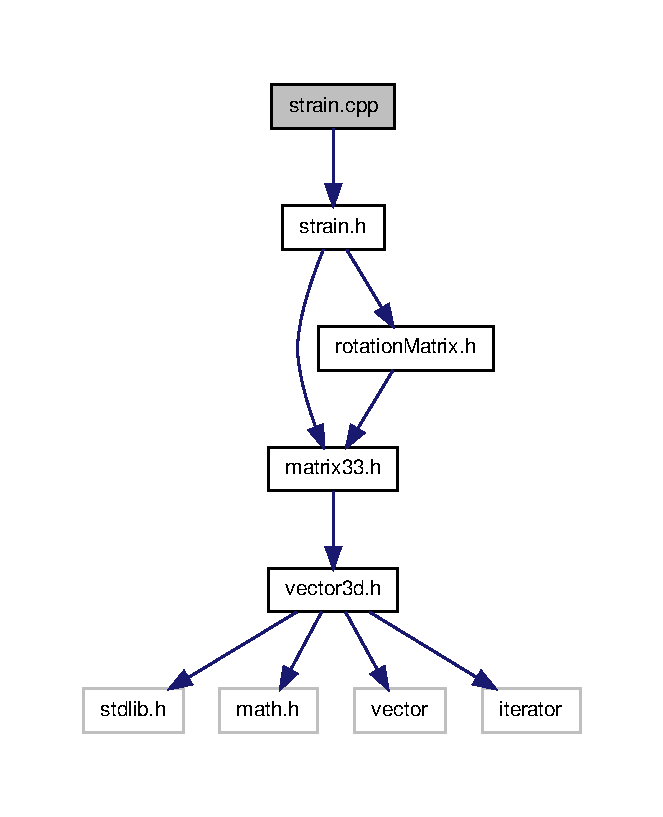
\includegraphics[width=318pt]{d1/da4/strain_8cpp__incl}
\end{center}
\end{figure}


\subsection{Detailed Description}
Definition of the member functions if the \hyperlink{classStrain}{Strain} class. \begin{DoxyAuthor}{Author}
Adhish Majumdar 
\end{DoxyAuthor}
\begin{DoxyVersion}{Version}
1.\-0 
\end{DoxyVersion}
\begin{DoxyDate}{Date}
05/06/2013
\end{DoxyDate}
This file defines the member functions of the \hyperlink{classStrain}{Strain} class for the strain tensor. 

Definition in file \hyperlink{strain_8cpp_source}{strain.\-cpp}.


\hypertarget{strain_8h}{\section{strain.\-h File Reference}
\label{df/dc2/strain_8h}\index{strain.\-h@{strain.\-h}}
}


Definition of the \hyperlink{classStrain}{Strain} class.  


{\ttfamily \#include \char`\"{}matrix33.\-h\char`\"{}}\\*
{\ttfamily \#include \char`\"{}rotation\-Matrix.\-h\char`\"{}}\\*
Include dependency graph for strain.\-h\-:\nopagebreak
\begin{figure}[H]
\begin{center}
\leavevmode
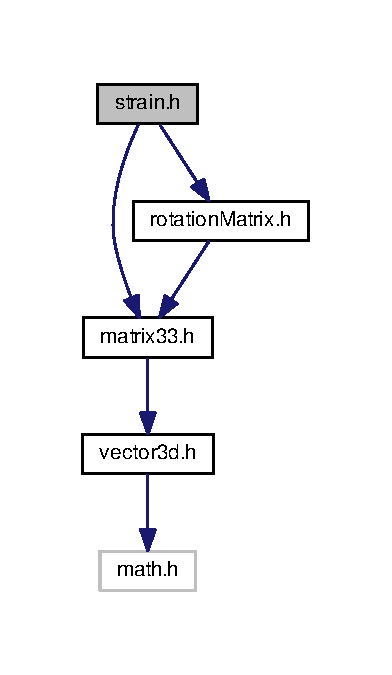
\includegraphics[width=188pt]{df/dd8/strain_8h__incl}
\end{center}
\end{figure}
This graph shows which files directly or indirectly include this file\-:\nopagebreak
\begin{figure}[H]
\begin{center}
\leavevmode
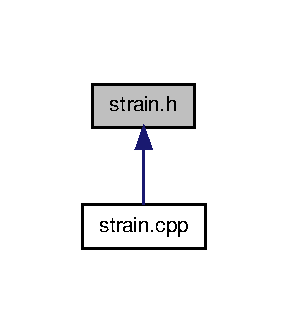
\includegraphics[width=138pt]{d0/d58/strain_8h__dep__incl}
\end{center}
\end{figure}
\subsection*{Data Structures}
\begin{DoxyCompactItemize}
\item 
class \hyperlink{classStrain}{Strain}
\begin{DoxyCompactList}\small\item\em \hyperlink{classStrain}{Strain} class to represent the strain tensor. \end{DoxyCompactList}\end{DoxyCompactItemize}


\subsection{Detailed Description}
Definition of the \hyperlink{classStrain}{Strain} class. \begin{DoxyAuthor}{Author}
Adhish Majumdar 
\end{DoxyAuthor}
\begin{DoxyVersion}{Version}
0.\-0 
\end{DoxyVersion}
\begin{DoxyDate}{Date}
25/04/2013
\end{DoxyDate}
This file defines the \hyperlink{classStrain}{Strain} class for the strain tensor. 

Definition in file \hyperlink{strain_8h_source}{strain.\-h}.


\hypertarget{stress_8cpp}{\section{stress.\-cpp \-File \-Reference}
\label{d4/d58/stress_8cpp}\index{stress.\-cpp@{stress.\-cpp}}
}


\-Definition of the member functions if the \hyperlink{classStress}{\-Stress} class.  


{\ttfamily \#include \char`\"{}stress.\-h\char`\"{}}\*
\-Include dependency graph for stress.\-cpp\-:
\nopagebreak
\begin{figure}[H]
\begin{center}
\leavevmode
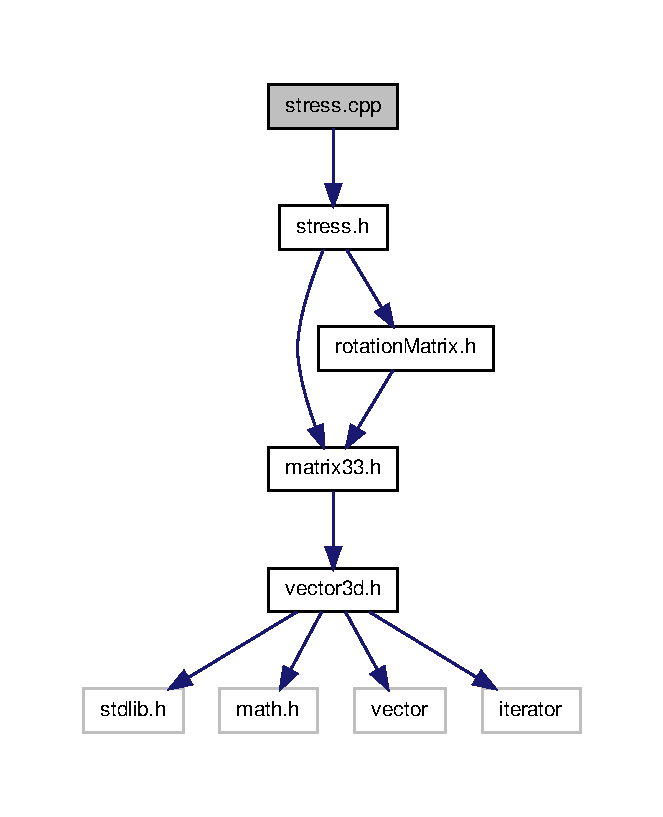
\includegraphics[width=188pt]{d0/d28/stress_8cpp__incl}
\end{center}
\end{figure}


\subsection{\-Detailed \-Description}
\-Definition of the member functions if the \hyperlink{classStress}{\-Stress} class. \begin{DoxyAuthor}{\-Author}
\-Adhish \-Majumdar 
\end{DoxyAuthor}
\begin{DoxyVersion}{\-Version}
0.\-0 
\end{DoxyVersion}
\begin{DoxyDate}{\-Date}
22/04/2013
\end{DoxyDate}
\-This file defines the member functions of the \hyperlink{classStress}{\-Stress} class for the stress tensor. 

\-Definition in file \hyperlink{stress_8cpp_source}{stress.\-cpp}.


\hypertarget{stress_8h}{\section{stress.\-h File Reference}
\label{d2/d50/stress_8h}\index{stress.\-h@{stress.\-h}}
}


Definition of the \hyperlink{classStress}{Stress} class.  


{\ttfamily \#include \char`\"{}matrix33.\-h\char`\"{}}\\*
{\ttfamily \#include \char`\"{}rotation\-Matrix.\-h\char`\"{}}\\*
Include dependency graph for stress.\-h\-:
\nopagebreak
\begin{figure}[H]
\begin{center}
\leavevmode
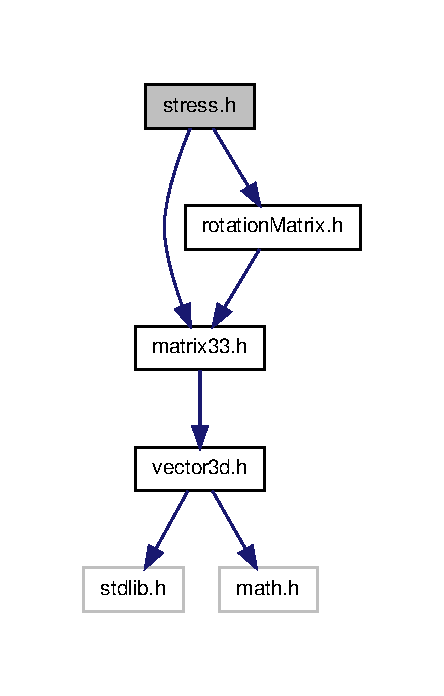
\includegraphics[width=213pt]{df/d2b/stress_8h__incl}
\end{center}
\end{figure}
This graph shows which files directly or indirectly include this file\-:
\nopagebreak
\begin{figure}[H]
\begin{center}
\leavevmode
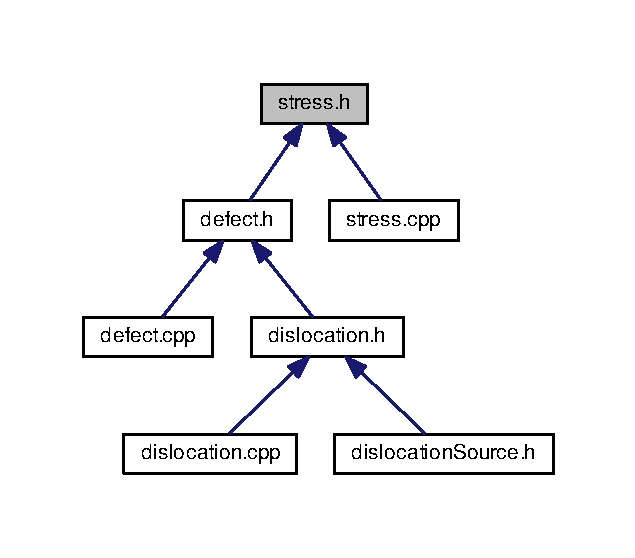
\includegraphics[width=350pt]{dc/d05/stress_8h__dep__incl}
\end{center}
\end{figure}
\subsection*{Data Structures}
\begin{DoxyCompactItemize}
\item 
class \hyperlink{classStress}{Stress}
\begin{DoxyCompactList}\small\item\em \hyperlink{classStress}{Stress} class to represent the stress tensor. \end{DoxyCompactList}\end{DoxyCompactItemize}


\subsection{Detailed Description}
Definition of the \hyperlink{classStress}{Stress} class. \begin{DoxyAuthor}{Author}
Adhish Majumdar 
\end{DoxyAuthor}
\begin{DoxyVersion}{Version}
1.\-0 
\end{DoxyVersion}
\begin{DoxyDate}{Date}
05/06/2013
\end{DoxyDate}
This file defines the \hyperlink{classStress}{Stress} class for the stress tensor. 

Definition in file \hyperlink{stress_8h_source}{stress.\-h}.


\hypertarget{vector3d_8cpp}{\section{vector3d.\-cpp File Reference}
\label{d7/d35/vector3d_8cpp}\index{vector3d.\-cpp@{vector3d.\-cpp}}
}


Definition of the \hyperlink{classVector3d}{Vector3d} class and its functions.  


{\ttfamily \#include \char`\"{}vector3d.\-h\char`\"{}}\\*
Include dependency graph for vector3d.\-cpp\-:\nopagebreak
\begin{figure}[H]
\begin{center}
\leavevmode
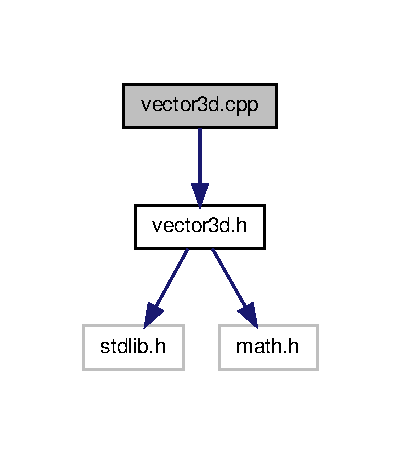
\includegraphics[width=154pt]{d5/d7b/vector3d_8cpp__incl}
\end{center}
\end{figure}


\subsection{Detailed Description}
Definition of the \hyperlink{classVector3d}{Vector3d} class and its functions. \begin{DoxyAuthor}{Author}
Adhish Majumdar 
\end{DoxyAuthor}
\begin{DoxyVersion}{Version}
0.\-0 
\end{DoxyVersion}
\begin{DoxyDate}{Date}
15/04/2013
\end{DoxyDate}
This file defines the \hyperlink{classVector3d}{Vector3d} class representing a single 3-\/dimensional vector in the simulation and its member functions and operators. 

Definition in file \hyperlink{vector3d_8cpp_source}{vector3d.\-cpp}.


\hypertarget{vector3d_8h}{\section{vector3d.\-h File Reference}
\label{d9/df8/vector3d_8h}\index{vector3d.\-h@{vector3d.\-h}}
}


Definition of the \hyperlink{classVector3d}{Vector3d} class.  


{\ttfamily \#include $<$stdlib.\-h$>$}\\*
{\ttfamily \#include $<$math.\-h$>$}\\*
{\ttfamily \#include $<$vector$>$}\\*
{\ttfamily \#include $<$iterator$>$}\\*
Include dependency graph for vector3d.\-h\-:
\nopagebreak
\begin{figure}[H]
\begin{center}
\leavevmode
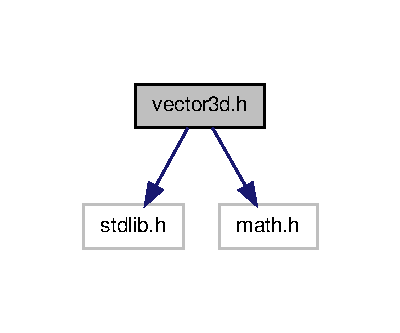
\includegraphics[width=318pt]{dc/db1/vector3d_8h__incl}
\end{center}
\end{figure}
This graph shows which files directly or indirectly include this file\-:
\nopagebreak
\begin{figure}[H]
\begin{center}
\leavevmode
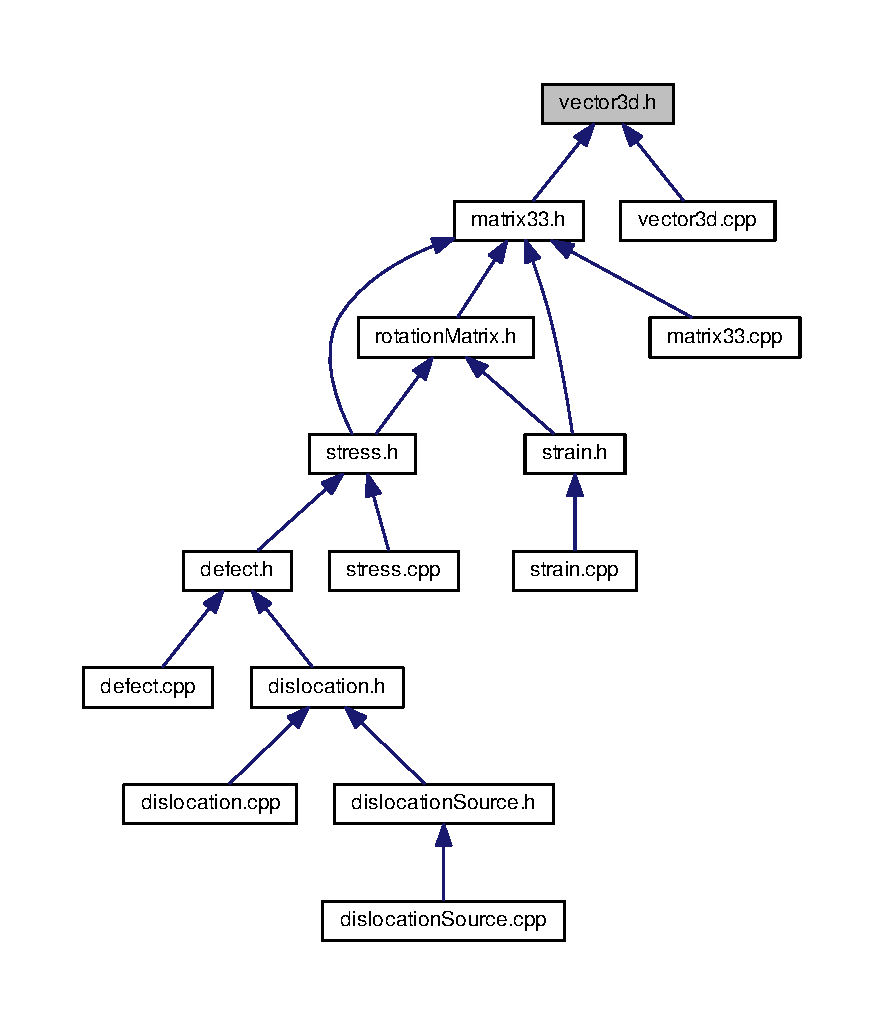
\includegraphics[width=350pt]{d3/dd7/vector3d_8h__dep__incl}
\end{center}
\end{figure}
\subsection*{Data Structures}
\begin{DoxyCompactItemize}
\item 
class \hyperlink{classVector3d}{Vector3d}
\begin{DoxyCompactList}\small\item\em \hyperlink{classVector3d}{Vector3d} class representing a single 3-\/dimensional vector in the simulation. \end{DoxyCompactList}\end{DoxyCompactItemize}


\subsection{Detailed Description}
Definition of the \hyperlink{classVector3d}{Vector3d} class. \begin{DoxyAuthor}{Author}
Adhish Majumdar 
\end{DoxyAuthor}
\begin{DoxyVersion}{Version}
1.\-0 
\end{DoxyVersion}
\begin{DoxyDate}{Date}
04/06/2013
\end{DoxyDate}
This file defines the \hyperlink{classVector3d}{Vector3d} class representing a single 3-\/dimensional vector in the simulation. 

Definition in file \hyperlink{vector3d_8h_source}{vector3d.\-h}.


\addcontentsline{toc}{part}{Index}
\printindex
\end{document}
